% Draft stages:
% BRAINSTORM - vague, unordered ideas of what and where things should go
% OUTLINE - Basic layout and section design
% DRAFT ALPHA - Information for all sections in a vaguely structured format
% DRAFT BETA - All sections revised into actual sentences
% DRAFT 0 - Chapter has all information with proper sentence structure and section transitions, along with needed figures
% DRAFT # - Anything after revising the #th series of comments from Steve
% DRAFT OMEGA 0 - The draft at which Steve decides things are ready for the committee
% DRAFT OMEGA # - Anything after revising the #th series of comments from the committee/higher bureaucracy

%NOTE: according to Steve, you can (and SHOULD) use "I" in the theory chapter. Indeed, use "I" as well literally anywhere I specifically was responsible for something. Do NOT use royal "we". Only use "we" in the context of what "we" the HDBS 4b or dihiggs group have done as a group, and only if you have explicitly defined who "we" are.

\documentclass[12pt]{report}

\usepackage{Dedman-Thesis-Latex-Template/sty/DL_thesis}  % Global Style for particular SMU College, e.g. DL_thesis.sty
\input{Dedman-Thesis-Latex-Template/latex/packages.tex}
% Load additional packages here.
% Be careful of the loading order with respect to packages.tex as conflicts can easily arise.
% This is not a part of the base template and so will never be overwritten during updates.
\usepackage{tikz}
\usepackage{graphicx}
\usepackage{tikz-feynman}
\usepackage{fontspec}
%\usepackage{mathtools}
\newfontface\mathcursivefont{Daytonia.otf}
\DeclareTextFontCommand{\mathcurse}{\mathcursivefont}
 % Uncomment to load additional user required packages
\input{Dedman-Thesis-Latex-Template/latex/preamble.tex}
\input{Dedman-Thesis-Latex-Template/latex/custom_commands.tex}
% Place your own personal commands here. 
% This is not a part of the base template and so will never be overwritten during updates.
 % Uncomment to use your own personal commands
\AuthorFirstName{Graduate}
\AuthorLastName{Student}
% \AuthorNameSuffix{Jr.}

% Title can be up to three lines of no more than 48 characters per line
% Write the title with the capitalization you want to be used in the abstract
\ThesisTitle{Smashy Physics:}{How I Pretended to Do More Smashing}{Using Smashy Math}
\GraduateDepartment{Physics}

\FirstDegree%
\FirstDegreeType{B.S.}
\FirstDegreeMajor{Physics}
\FirstDegreeUniversity{Undergraduate University}

\SecondDegree%
\SecondDegreeType{M.S.}
\SecondDegreeMajor{Physics}
\SecondDegreeUniversity{Southern Methodist University}

\ThesisDefenseDateYear{2022}
\ThesisDefenseDateMonth{April}
\ThesisDefenseDateDay{1}

\GraduationDateYear{2022}
\GraduationDateMonth{July}
\GraduationDateDay{1}

\SMUCollege{Dedman College}

% Committee
\AdvisorFullName{Dr.~Stephen Sekula}
\AdvisorTitle{Associate Professor}

\CommitteeMemberA{Dr.~Roberto Vega}
\CommitteeMemberTitleA{Professor}

\CommitteeMemberB{Dr.~Jingbo Ye}
\CommitteeMemberTitleB{Associate Professor}

\CommitteeMemberC{Dr.~External Member}
\CommitteeMemberTitleC{Assistant Professor}

\hypersetup{
 % Added more precise definition and options for Hyperref package.
 % Comment out or change hyperref preferences
 % \hypersetup should be loaded last
 bookmarksopen=true, % True: Open bookmark tree
 bookmarksnumbered=true, % True: put section numbers in bookmarks
 breaklinks=true, % True: split the url over multiple lines
 %   draft=true, % True: do not do any hyper linking
 filecolor=magenta, % Color of file links
 citecolor=blue, % Color of links to bibliography
 colorlinks=true, % False: boxed links; true: colored links
 linkcolor=blue, % Color of internal links
 linktocpage=true, % True: Makes the page number of TOC the link vs the text
 %   pagebackref=true, % True: Links references back to referring page
 pdfnewwindow=true, % True: URL links in new window
 plainpages=false, % True: do page number anchors as plain Arabic
 pdffitwindow=false, % Window fit to page when opened
 pdfmenubar=true, % Show Acrobat menu
 pdfstartview={FitH}, % Fits the width of the page to the window
 pdftoolbar=true, % Show Acrobat toolbar
 pdfauthor={Author}, % Author in PDF document properties
 pdfcreator={Author}, % Creator of the document in PDF document properties
 pdfkeywords={Keyword1} {Keyword2} {Keyword3} {Keyword4} {Author}, % List of keywords in PDF document properties
 pdfproducer={Producer}, % Producer of the document in PDF document properties
 pdfsubject={Subject}, % Subject of the document in PDF document properties
 pdftitle={Title of Dissertation}, % Title in PDF document properties
 unicode=false, % Non-Latin characters in Acrobat bookmarks
 urlcolor=cyan % Color of external links
}


\makeglossaries
\newglossaryentry{LHC}{
 text=LHC,
 long=Large Hadron Collider,
 name={\glsentrylong{LHC} (\glsentrytext{LHC})},
 first={\glsentryname{LHC}},
 sort={large hadron collider},
 description={Large Hadron Collider}
}

\newglossaryentry{thesis}{
 name=thesis,
 description={https://xkcd.com/1403/}
}


% \thesisdraft % uncomment if want draft printing

\begin{document}

\input{Dedman-Thesis-Latex-Template/latex/front_pages.tex}

\begin{thesis}

% Ch0: I'm... actually not using this right now. Maybe later?
% I'm trying to describe organically throughout the thesis.
%\chapter*{Preface}\label{chapter:preface}
% c.f. https://tex.stackexchange.com/a/222961/152544
\addcontentsline{toc}{chapter}{\protect\numberline{}Preface}

The following is a summary of useful concepts in high energy particle physics.

\section{Units}\label{section:units}

Discussion of units

\section{Coordinates}\label{section:coordinates}

\gls{LHC} coordinate systems

\section{Statistics}\label{section:statistics}

Statistics in particle physics


% Ch1: Introduction - DRAFT 2
\chapter{Introduction}\label{chapter:introduction}

%The basic structure of every lab report you've ever done is: 
%    introduction,
%    theory,
%    experimental setup,
%    procedure,
%    results,
%    conclusion.
%
%This thesis is essentially following that same format:
%    Introduction,
%    Standard Model... and Signal modelling? (theory),
%    LHC and ATLAS and Trigger (experimental setup)
%    Reconstruction, Selection, Background Estimation (procedure)
%    results (...)
%    conclusion

The Higgs Boson was proposed as a fundamental particle in 1964,
    and has been a driving factor in particle physics research ever since.
Though it was jointly discovered in 2012 by the ATLAS and CMS collaborations,
    there are still a number of properties of the Higgs which have yet to be measured.
Chief among these are two of the Higgs' self-coupling constants, \kl and \kvv,
    which determine how strongly the Higgs interacts with both itself and with vector bosons.
This analysis performs a search for the rare,
    as-yet unseen diHiggs interaction in order to set tighter constraints on these coupling values.
The search utilizes the Vector Boson Fusion production mechanism of the diHiggs process,
    identifying the process in the 4b final state.
This is performed using 126 $\textit{fb}^{-1}$ of data from Run 2 of ATLAS.

This thesis will begin by first explaining the importance of the Higgs Boson to the field of particle physics,
    as well as the relevance of the aforementioned \kl and \kvv coupling constants.
I will then describe the physical effects of these constants,
    and how those effects can be exploited in order to make measurements of them.
These topics comprise Chapter \ref{chapter:theory}.
Following from the theoretical discussion, I will discus the experimental equipment and setup used to perform the  measurments.
The experimental setup is discussed across three chapters.
Chapter \ref{chapter:lhc} discusses the Large Hadron Collider, the machine which generates the conditions necessary to produce diHiggs process.
Actual observation of the process once generated is carried out by the ATLAS particle detector array and its Trigger system,
    described in Chapters \ref{chapter:atlas} and \ref{chapter:trigger}.
The reconstruction process, described in Chapter \ref{chapter:reconstruction},
    entails how data observed by ATLAS is analyzed in order to determine which physics processes occured during the myriad observed interactions.
Background processes are removed from the data set using a selection procedure explained in Chapter \ref{chapter:selection},
    and the contribution of the background events which remain is estimated using data-driven technique cataloged in Chapter \ref{chapter:background}. 
The background estimation process makes use of a neural network reweighting procedure, which I personally configured and ran the training for.
My primary contribution to the analysis however, comes in the form of the signal model that constitutes the hypothesis for the behaviour of the Higgs Boson.
The signal model makes use of a Monte-Carlo sample combination technique, which I developed and optimized in the context of the \vbfproc process.
This is elaborated upon in Chapter \ref{chapter:signal}.
Finally, in Chapter \ref{chapter:results}, this hypothesis alongside the background estimate are compared against the data observed from ATLAS,
    in order to make constraints on the diHiggs self-coupling constants.



%This is the first chapter of the \gls{thesis}.~\cite{Aaboud:2016mmw,Bruning:782076}

\section{Creating Figures}\label{sec:figures}
\begin{figure}[htpb]
 \centering
 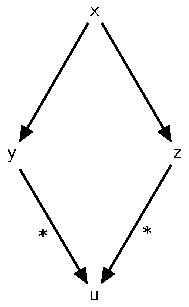
\includegraphics{introduction/example.pdf}
 \caption[Example placeholder figure with a citation~\cite{Higgs:1964ia} and shorter List of Figures caption.
  The List of Figures is protected from first use of glossary entries or acronyms like \acrlong{LHC}.]{%
  This is a placeholder figure to act as an example.
  Here we cite a new reference in the caption to demonstrate that given the package configuration our order of references will not be distributed by the table of contents~\cite{Higgs:1964ia}.}\label{fig:test_figure}
\end{figure}

As can be seen in \Cref{fig:subfigure_example}, the subfigures are independent of each other such that \Cref{fig:subfigure_1} and \Cref{fig:subfigure_2} can be accessed separately.

\begin{figure}[htbp]
 \centering
 \begin{subfigure}[t]{0.48\textwidth}
  \centering
  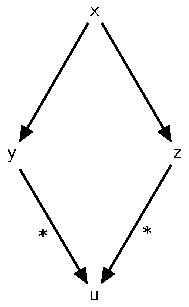
\includegraphics[width=0.3\textwidth]{introduction/example.pdf}
  \caption[Short List of Figures captions work with subfigures too.]{%
   This is the first figure of two, in this example, and its own independent subfigure.}
  \label{fig:subfigure_1}
 \end{subfigure}%
 \quad
 \begin{subfigure}[t]{0.48\textwidth}
  \centering
  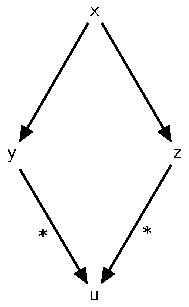
\includegraphics[width=0.3\textwidth]{introduction/example.pdf}
  \caption[Which makes the List of Figures readable and actually helpful.]{%
   As the \texttt{t} alignment option was chosen for the subfigures, they are still properly aligned vertically even though this caption is longer.}
  \label{fig:subfigure_2}
 \end{subfigure}
 \caption{An example of a figure that consists of two subfigures.}
 \label{fig:subfigure_example}
\end{figure}

As an example of an equation formatted in ``\href{https://www.overleaf.com/learn/latex/Display_style_in_math_mode}{display style}'' the equation for the fiducial cross section from~\cite{Aaboud:2016mmw} is reproduced as \Cref{eq:fiducial_cross_section}:
\begin{equation}
 \sigma_{\mathrm{inel}}^{\mathrm{fid}} \left(\zeta > 10^{-6}\right) = \frac{N - N_{\mathrm{BG}}}{\epsilon_{\mathrm{trig}} \times \mathcal{L}} \times \frac{1 - f_{\zeta < 10^{-6}}}{\epsilon_{\mathrm{sel}}}
 \label{eq:fiducial_cross_section}
\end{equation}

\section{Creating Tables}\label{sec:tables}

To create tables in \LaTeX{} it is highly recommended to use the \href{https://www.ctan.org/pkg/booktabs}{\texttt{booktabs}} package.
It allows for very elegant and clean table creation, such as \Cref{table:natural_units}.
If you want to create a table quickly, or have a CSV file that you'd like to quickly turn into a table there are various \href{https://www.tablesgenerator.com/}{online \LaTeX{} table generators}.

\begin{table}[htpb]
 \centering
 \caption[Common quantities in particle physics in natural and SI units.]{%
  Common quantities in particle physics given in both natural units and SI units.}
 \begin{tabular}{@{}llll@{}} \toprule
  Quantity         & Natural Units                 & Natural Units (dimensionful)            & SI Units                                              \\ \midrule
  Speed            & $1$                           & $c$                                     & $3.0\times 10^{8}~\mathrm{m}/\mathrm{s}$              \\
  Angular Momentum & $1$                           & $\hbar$                                 & $10^{34}~\mathrm{m}^2 \,\mathrm{kg}/\mathrm{s}$       \\
  Energy           & $\mathrm{GeV}$                & $\mathrm{GeV}$                          & $1.6\times 10^{-10}~\mathrm{J}$                       \\
  Momentum         & $\mathrm{GeV}$                & $\mathrm{GeV}/c$                        & $1\times 10^{-19}~\mathrm{kg}\,\mathrm{m}/\mathrm{s}$ \\
  Mass             & $\mathrm{GeV}$                & $\mathrm{GeV}/c^{2}$                    & $1.8\times 10^{-27}~\mathrm{kg}$                      \\
  Time             & $1/\mathrm{GeV}$              & $\hbar/\mathrm{GeV}$                    & $6.6\time 10^{-25}~\mathrm{s}$                        \\
  Length           & $1/\mathrm{GeV}$              & $\hbar c/\mathrm{GeV}$                  & $2\times 10^{-16}~\mathrm{m}$                         \\
  Electric Charge  & $1$                           & $e/\sqrt{4\pi \alpha_{\mathrm{em}}}$    & $5.3\times 10^{-19}~\mathrm{C}$                       \\
  Magnetic Field   & $\left(\mathrm{GeV}\right)^2$ & $\left(\mathrm{GeV}\right)^2/\hbar c^2$ & $5\times 10^{16}~\mathrm{T}$                          \\
  \bottomrule
 \end{tabular}\label{table:natural_units}%
\end{table}

Good table design requires some thought and work, so it may be worth a look through some examples:
\begin{itemize}
 \item \href{https://tex.stackexchange.com/questions/238503/tip-on-how-to-make-a-visually-good-table}{TeX StackExchange: Tip on how to make a visually good table}
 \item \href{https://twitter.com/edwardtufte/status/451820483109847040?lang=en}{Edward Tufte endorsed} example from \href{http://static1.squarespace.com/static/56713bf4dc5cb41142f28d1f/t/56fd4c83746fb9261146eed5/1459440776291/ClearOffTheTableMd.gif}{Darkhorse Analytics}
\end{itemize}

\section{Dealing with Widows and Orphans}\label{sec:widos_and_orphans}

To reduce the difficulty of dealing with widowed text (the last line of a paragraph at the start of a page) and orphaned text (the first line of paragraph at the end of a page) the \href{https://ctan.org/pkg/nowidow?lang=en}{\texttt{nowidow}} package is used.
However, that doesn't solve the issue of orphaned section titles.
The user must manually do this, but the following \href{https://texfaq.org/FAQ-widows}{simple advice from \TeX{} FAQ} is recommended:

\begin{quote}
 Once you've exhausted the automatic measures, and have a final draft you want to ``polish'', you should proceed to manual measures.
 To get rid of an orphan is simple: precede the paragraph with \texttt{\textbackslash clearpage} and the paragraph can’t start in the wrong place.
\end{quote}



% Ch2: Standard Model Discussion - DRAFT 2
\chapter{Theory}\label{chapter:theory}

%So what even do I need to talk about here?
%
%Final goal = Higgs (final goal should actually probably be di-higgs and a discussion of the relevence of this...)
%    What: What is the Higgs?
%    Why: Why do we care about it? It gives things mass and messes with the electroweak interaction
%    When: In what contexts does the Higgs become relevant? The mass of (most) elementary particles and the weak force being weak
%    Where: Where does the higgs fit into the SM? The "Higgs Mechanism"
%    How: How does the higgs mechanism work?

\section{Introduction}

    The Higgs Boson sits as the crown jewel of a grand overarching theory of the behaviour of the universe,
        known as the Standard Model of Particle Physics.
    While its recent discovery has shed light on many of its key properties,
        there are still many details of its nature that are as yet uncomfirmed.
    In this chapter, I want to explain what these properties are and how they can be further studied.
    Moreover, I want to justify why the Higgs is so important as to be worth studying in the first place.
    And to understand the importance of the Higgs Boson, one must understand the structure of the Standard Model itself.

    The structure of the following sections will begin with a discussion of the purpose and fundamental structure of the Standard Model.
    I will follow this with an introduction to the mathematical formalism the Standard Model is based around,
        involving Group Theory, the calculus of variations, and symmetry.
    Here I will introduce the reason for the original postulation of the Higgs, what it is, how it works, and how it fits into the Standard Model.
    Finally, I will motivate further study into the Higgs and provide a technique to perform this study.


%Matter and Forces
%I need to discuss the elementary particles and their organization before I can really discuss the gauge fields.
%Might as well do it here first and foremost
\section{The Standard Model of Particle Physics}
    
    At its core, the Standard Model of Particle Physics is a description of the behaviour and interaction of matter.
    First and foremost then, I want to discuss what this matter actually is.
    All matter can be described as a specific type of elementary particle called a fermion,
        defined by the fact that it contains no discernable substructure and possesses an intrinsic spin of 1/2.
    These particles all have different masses, and are able to interact with each other through three ``fundamental interactions''.
    The three fundamental interactions (more commonly called ``Fundamental Forces'') are known as
        the Electromagnetic, Weak, and Strong interactions (gravity is entirely absent in the Standard Model).
    All the interactions have an associated ``charge'' which can be ascribed to different particles,
        and which govern how strongly that particle can interact with similarly charged particles.
    The various fermions are distinct largely because of the charges they carry.

    \begin{figure}[h!]
        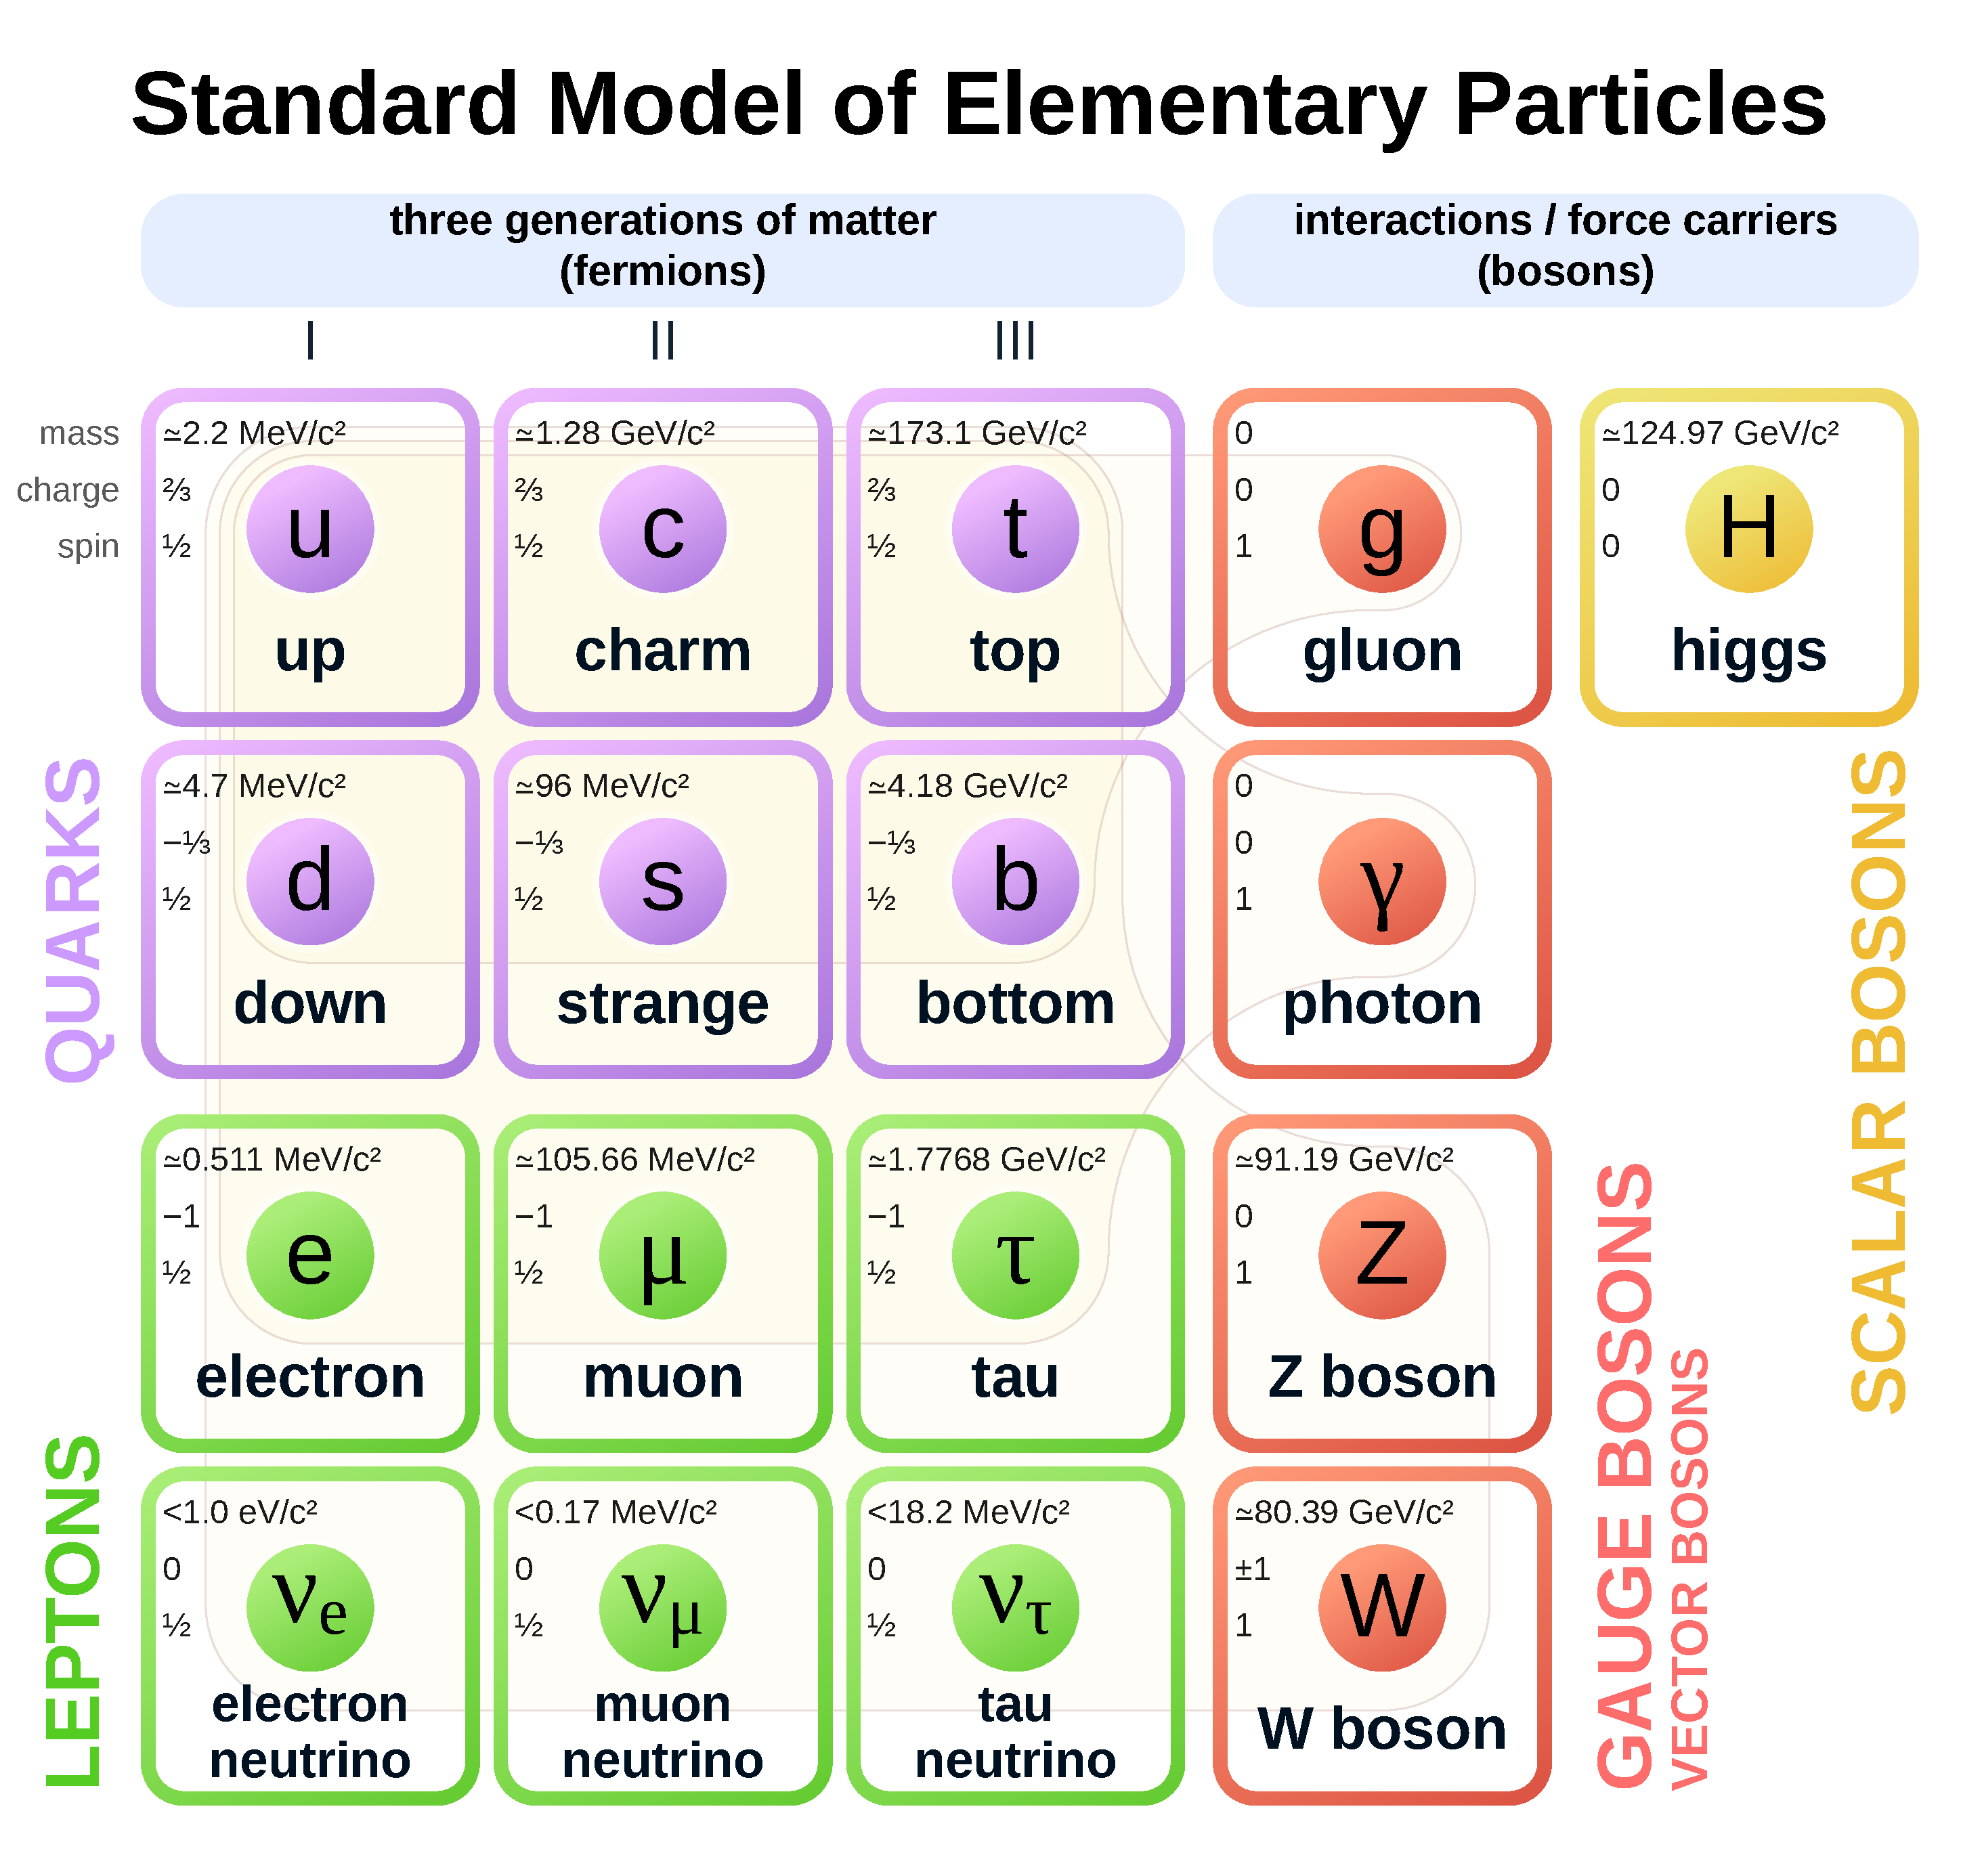
\includegraphics[width=\linewidth,height=\textheight,keepaspectratio]{theory/Standard_Model_of_Elementary_Particles}
        \caption{I'm probably going to need to find something else since this came from wikipedia. I just wanted a placeholder}
        \label{fig:sm_particles}
    \end{figure}
        

    There are twelve distinct elementary fermions (see Figure \ref{fig:sm_particles}),
        which are split evenly into two subgroups, called quarks and leptons.
    Quarks have a charge of 1 with the Strong interaction,
        while leptons have a charge of 0 (and thus cannot interact via the Strong Interaction at all).
    Both classes of particles, quarks and leptons, are divided into three ``generations'' of progressively heavier particles.
    Each generation thus consists of two quarks and two leptons.
    These pairs, called ``doublets'', behave the same across all generations.
    Among the quarks, every generation contains a doublet of an up-type quark (Up, Charm, Top) with electromagnetic charge of 2/3,
        and a down-type quark (Down, Strange, Bottom) with EM charge of -1/3.
    For leptons, each doublet consists of a particle with EM charge of -1, and a neutrino with EM charge of 0.

    In addition to the fermions, there is also an entirely seperate class of particles, called gauge bosons,
        which play a fundamental role in the aforementioned interactions.
    However, the nature of these particles will be discussed later.
    Now, with the enumeration of the various particles complete, it is time to begin the discussion of the Standard Model itself,
        which will serve to explain how these fermions interact with each other.



\section{Composition of Matter: Fields and Dirac Spinors}

    %Fields are a thing.
    The description of matter is governed by the formalism of Quantum Field Theory, which describes particles as pertubations of an overall particle \textit{field}.
    %They're kinda like quantum waves, but not.
    A particle field $\varphi$, describes every particle of the same type at once,
        and particle states $\ket{\varphi}$ correspond to the number of that kind of particle that exists at a given moment.
    The equation of motion used to describe a field varies depending on the properties of the field.
    For a scalar (spinless) field, \phi, the equation of motion is the Klein-Gordon Equation
    \begin{equation} \begin{split}
        p^2 \phi = m^2 \phi
        \\(p^2 - m^2) \phi = 0
    \end{split} \end{equation}
    Recalling the covariant, natural units, quantum mechanical definition of momentum as $p^u = i\partial^u$,
        this can also be written as
    \begin{equation} \begin{split}
        (p^2 - m^2) \phi = 0 \rightarrow (\partial^\mu \partial_\mu + m^2) \phi = 0
    \end{split} \end{equation}

    The Klein-Gordan Equation will be used later when describing the Higgs Field,
        but for now the more important equation is that used for fermions, $\psi$,
        called the Dirac Equation
    \begin{equation}
        (\gamma^\mu p_\mu - m) \psi = 0
        (i\gamma^\mu \partial_\mu  - m) \psi = 0
    \end{equation}

    The Dirac Equation seeks to make the equation of motion first order (i.e.\ only one derivative),
        as this permits a representation of a spinor field.
    Doing this comes with a cost however, as momentum $p_\mu$ is a four-vector, but mass is a scalar.
    The resolution to this problem is a set of four, 4x4 matrices, $\gamma^\mu$, called the gamma matrices.


    %Fields don't describe a single particle, but all particles of the same type at once.
    %Field states are just a count of how many of that particles exist at a given time.
    %Scalar particles are described by Klein Gordon Equation.
    %Spin 1/2 particles are described by dirac equation.
    %It's first order in p, but this requires the gamma matrices.
    %Matrices take many forms, but one of the most revealing is the Weyl, or Chiral, form.
    %Do some math to show fields in chiral form, to show Chirality.


    %It takes from quantum mechanics the uncertainty principle, and from relativity the mass/energy equivalence 
    %It takes from quantum mechanics the wave-like description of position and momentum, along with the uncertainty principle.
    %From special relativity it incorporates the equivalence of space and time, the constance of the speed of light,
    %    and the exchange between mass and energy.
    %Combining the energy/time uncertainty principle with mass/energy equivalence in particular
    %    has the outcome that the number of particles for a given system need not remain constant.
    %To account for this, particles are not described as waves as with the Schrodinger Equation, but rather as ``fields''.
    %A fermion field, $\psi$, does not describe a single particle, but rather all possible fermion for the same kind of particle.
    %For instance, there is a seperate fermion field to describe electrons, up-quarks, and so forth.

    
    describe gamma matrices

    describe anti particle psi bar

    describe chiral representation
    

    %What is the Universe made of (If you stick to this format at all, keep this section brief):

    %%Position and Momentum: Quantum Mechanics
    %   The position and momentum of that matter:
    %       Described via the Canonical Commutation Relation and the formalism of Quantum Mechanics
    %       (explain 'h' here?)
    %   Describe basic function of schrodinger equation and why it fails

    %%Space and Time: Special Relativity
    %   The space-time in which that matter resides: described by the Minkowski Metric Tensor.
    %    Explain what the metric tensor means and maybe covariant notation,
    %    as well as mass-energy-momentum equivalence,
    %    and also the speed of light
    %    Reformat schrodinger equation as klein gordon and show how this also fails


    %%Particles and Fields: Quantum Field Theory
    %   A description of how the position of matter can change: Described by the Dirac Equation.
    %    A unification of Quantum Mechanics and Special Relativity
    %    (maybe go through the derivation, starting from schrodinger -> klein-gordon -> dirac and why each fails)
    %    Describe Weyl Spinors and Chiral representation (peskin pg 64)



\section{Generating Motion: Group Theory and Transformations}

    The Dirac Equation provides a description of matter.
    The next key piece of the Standard Model is a description of motion itself.
    For this, I will need to introduce Group Theory.

    A function can be altered using a \textit{transformation operator}.
    A simple example of this would be a function $x(t)$, 
        which (assuming constant velocity) can be transformed into a time $\Delta t$ in the future as
    \begin{equation}
    x(t) \rightarrow x'(t) = x(t) + v \Delta t
    \end{equation}
    Noting that $v$ is just $\frac{d}{dt} x(t)$, this can be rewritten as
    \begin{equation}
    x(t) \rightarrow x'(t) = x(t) + \Delta t \frac{d}{dt} x(t) = \left(1+\Delta t \frac{d}{dt}\right) x(t)
    \end{equation}

    This term $\left(1+\Delta t \frac{d}{dt}\right)$ is the classical time-translation operator.
    Notice the assumption of \textit{constant velocity} though.
    If velocity were not constant, this operator would be invalid, except for in the specific case in which $\Delta t$ is infinitesimal.
    \begin{equation}
    x(t) \rightarrow x'(t) = \lim_{\delta t \to 0} \left(1+\delta t \frac{d}{dt}\right) x(t)
    \end{equation}

    To produce a more general finite operator however, I can just apply the infinitesimal operator an infinite number of times
    \begin{equation} \begin{split}
    x(t) \rightarrow x'(t) &= \lim_{\delta t \to 0} \left(1+\delta t \frac{d}{dt}\right)\left(1+\delta t \frac{d}{dt}\right)\left(1+\delta t \frac{d}{dt}\right)...\ x(t)
    \\x(t) \rightarrow x'(t) &= \lim_{N \to \infty} \lim_{\delta t \to 0} \left(1+\delta t \frac{d}{dt}\right)^N x(t)
    \\x(t) \rightarrow x'(t) &= e^{\Delta t \frac{d}{dt}} x(t)
    \end{split} \end{equation}

    Where $\Delta t$ is again a finite time transformation,
        and I have compressed the infinite product of terms using the power series expansion of the exponential function.
    In order to use this classical operator in quantum field theory, it must have a complex factor `$i$' associated with it
    \begin{equation} \begin{split}
    x(t) \rightarrow x'(t) = e^{i\Delta t \frac{d}{dt}} x(t)
    \end{split} \end{equation}



     

    %A ``group'' is a set of elements which can be ``multiplied'' according to some rule,
    %    and which satisfies the four conditions of:
    %        \begin{itemize}
    %            \item Closure - the product of any two elements of the group are still in that group;
    %            \item Associativity - $(a \times b)\times c = a\times(b \times c)$;
    %            \item Identity - there is some element in the group $I$ for which $I \times a=a$;
    %            \item and Inversion - every element $a$ has an inverse $a^{-1}$ such that if $b \times a = c$ then $c \times a^{-1} = b$.
    %        \end{itemize}

    %If the group operation is commutative ($ab=ba$) then the group is ``Abelian''; if not, it is ``non-Abelian''.


    \cite{Cheng_book}

\section{Restricting Motion: The Lagrangian and Symmetry}
    
    The Dirac Equation describes the equation of motion of a single field.
    I need a way to describe the collective motion and interactions of many fields at once.
    Enter the Lagrangian.

    

    %Explain how motion is described by a lagrangian of fields. 
    %Minization of Action.
    %Equations of motion derived from Euler-Lagrange Equations.
    %The lagrangian takes the form it does in order to satisfy poincare symmetry.

    %Discuss Noether's Theorem; refer to Halzen pg 314 (djvu=331) or, maybe better, Sredneki pg 144).
    %    ... Wait, do I even need to mention noether's theorem?
    %    I don't think it's actually a factor in producing the higgs... which makes me slightly sad :-(

    %I also should maybe end this with a discussion of how forces aren't really a thing
    %    and particles in field theory exchange momentum by merely bumping into other particles.
    %Maybe, *maybe**** (maybe not) give a toy example lagrangian showing a particle which can interact with itself via a three-point vertex or something.
    %Note the basic symmetries that the basic lagrangian must satisfy (hence group theory going first)
    %
    %Should I also discuss renormalizability? (Peskin pg 80/101djvu)
    %Basically, all lagrangians must be renormalizable.
    %Renormalizability just means that the lagrangian doesn't explode from the unconstrained nature of virtual particles.
    %So infinite-mass virtual particles should not break a renormalizeable lagrangian.
    \cite{Halzen_book}


\section{Transferring Motion: Gauge Symmetry}
    Gauge Transformations are ones where the transformation is imposed differently at each point in spacetime.
    Trying to impose a constraint on the Lagrangian that it be symmetric under gauge transformations would surely cause all manner of complications.
    Obviously, this is exactly what nature seems to have chosen to do.

    Gauge symmetries; U1, SU(N).
    The effects of imposing gauge symmetries on the Lagrangian, and the advent of the gauge bosons and their forces.
    how do gauge bosons come out from symmetries.

    U(1) is phase transforms

    SU(2) is based on 2x2 pauli matrices and thus requires pairing generations of particles together;
        so up and down-type quarks are paired together and charged leptons with neutrinos.
    It treats left handed fields as these doublet pairs,
        but works in "singlet representation" (which means it basically is just gone) for right-handed fields

    SU(3) is based on a 3x3 structure constant, and thus acts on all three "generations" of quarks as one 3x1 vector.
    It is a singlet (read, it literally doesn't matter) for leptons.
    
    \cite{Osborn_notes}
    \cite{Peskin_book}
    \cite{Halzen_book}



\section{Origin of Mass: The Higgs Mechanism}\label{sec:higgs_mechanism}

    The derivation provided throughout the next three sections seeks to explain
        how the Higgs mechanism is able to preserve the theory of gauge symmetry
        and largely follows the process laid out by Peskin\cite{Peskin_book}.
    To start, introduce a massless, scalar field $\phi$.
    The equation of motion for this field will be the Klein-Gordon equation
    \begin{equation} \begin{split}
        p^2 \phi &= m^2 \phi
        \\(p^2 - m^2) \phi &= 0
        \\(\partial^\mu \partial_\mu + m^2) \phi &= 0
        \\\partial^\mu \partial_\mu \phi &= 0,\; m\to0
        \,.
    \end{split} \end{equation}

    By default, the Lagrangian for this field will be a trivial kinetic-only term
    \begin{equation}
        \Lag = K_{\phi} = \frac{1}{2} (\partial_{\mu} \phi)^2
        \,.
    \end{equation}
    Next, introduce a quartic potential $U(\phi) = -\frac{1}{2} \mu^2 \phi^2 + \frac{1}{4} \lambda \phi^4$.
    Now the Lagrangian takes the form
    \begin{equation}
        \Lag = K_{\phi} - U_{\phi} = \frac{1}{2} (\partial_{\mu} \phi)^2 
            +\frac{1}{2} \mu^2 \phi^2 - \frac{1}{4} \lambda \phi^4
        \,.
    \end{equation}
    Such a potential will result in a Hamiltonian which is symmetric about a local maximum at $\phi=0$.
    The Hamiltonian will have two minima to either side of $\phi=0$, at points $\pm v = \pm \frac{\mu}{\sqrt{\lambda}}$.

    This is a small, seemingly innocuous change, so allow me to emphasize:
        this quartic potential is the linchpin of the entire Standard Model,
        and the origin of nearly all fundamental mass\footnote{
            Where ``fundamental mass'' refers to the mass of fundamental particles
                (except for that of neutrinos; the origin of neutrino mass is still a point of active research).
            Gluon binding energy is the actual source of most mass found in the baryonic matter of the universe
                (baryonic matter as opposed to \textit{dark matter},
                which is actually the vast majority of all mass in the universe
                and which is \textit{another} field of active research).
        } in the universe as it is currently understood.
    The reason for such a dramatic outcome begins with the fact that
        a system in such a potential will invariably fall into one of these minima.
    The Lagrangian can be rewritten from the perspective of one of these minima (e.g.\ $+v$),
        by substituting in a shifted field $h$, where $\phi(x)=v+h(x)$.
    \begin{equation} \begin{split} \label{eq:basic_higgs}
        \Lag & = \frac{1}{2} (\partial_{\mu} h)^2
            - \mu^2 h^2
            -\sqrt{\lambda} \mu h^3
            - \frac{1}{4} \lambda h^4 
            + \frac{\mu^4}{4 \lambda} \\
         & = \frac{1}{2} (\partial_{\mu} h)^2
            - m^2_{h} h^2
            -\sqrt{\lambda} \mu h^3
            - \frac{1}{4} \lambda h^4
        \,.
    \end{split} \end{equation}
    With the latter equation taking the form of a now massive field $h$ with both a three and four point self-coupling vertex
        (the constant potential term $\frac{\mu^4}{4 \lambda}$ is simply dropped, as potential energy is relative).
    This is the mechanism used to take a massless, symmetric field and convert it to a massive, asymmetric form.
    In the next section, I will show how the same scalar field can induce mass in fields other than itself.



\section{Breaking Symmetry: GWS Theory}

    Based on the theory formulated by Glashow, Weinberg, and Salam (GWS Theory),
        I will now give the scalar field a complex phase and spinor components:
    \begin{equation}
        \vec{\phi}(x) = \frac{1}{\sqrt{2}} \tinymatrix{\phi_1 \\ \phi_2}
        \,.
    \end{equation}
    $\vec{\phi}$ is still a scalar in space-time, but now also has vector components in the $SU(2)$ subspace.
    As with the Dirac fields, I will then impose $U(1) \times SU(2)$ gauge symmetry on the field, so it transforms as
    \begin{equation}
        \vec{\phi}(x) \rightarrow e^{i \alpha^a \tau^a} e^{i \beta/2 } \vec{\phi}(x)
        \,.
    \end{equation}
    The additional symmetries will in general complicate matters significantly,
        but they do allow for one simplification which I will immediately utilize.
    Regardless of symmetries, any arbitrary vector such as $\vec{\phi}$ can be written as a unitary transformation $U(x)$ operating on a simpler single-valued vector
    \begin{equation}
        \vec{\phi}(x) = \frac{1}{\sqrt{2}} \tinymatrix{\phi_1 \\ \phi_2} = \frac{1}{\sqrt{2}} U(x) \tinymatrix{0 \\ \phi}
        \,.
    \end{equation}
    Courtesy of the newly added gauge freedom, this field can be rotated through $SU(2) \times U(1)$ space freely without affecting the Lagrangian.
    A particularly convenient rotation to perform then, is one in alignment with the orientation of $U(x)$, such that $U(x)$ vanishes
    \begin{equation} \begin{split}
        \vec{\phi}(x) \rightarrow \vec{\phi}'(x) 
            &= U^{-1}(x) \vec{\phi}(x)
            = \frac{1}{\sqrt{2}} U^{-1}(x) U(x) \tinymatrix{0 \\ \phi}
            = \frac{1}{\sqrt{2}} \tinymatrix{0 \\ \phi} \\
        \vec{\phi}'(x) &= \frac{1}{\sqrt{2}} \tinymatrix{0 \\ \phi}
        \,.
    \end{split} \end{equation}
    This orientation is referred as the \textit{Unitary Gauge}, and will be used for the rest of the chapter.

    \begin{figure}[h!]
        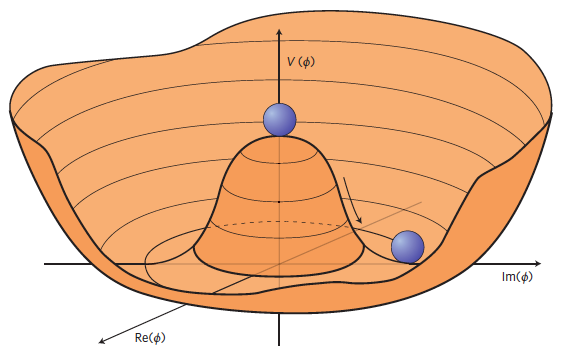
\includegraphics[width=\linewidth,height=\textheight,keepaspectratio]{theory/higgspotential}
        \caption{A two-dimensional representation of the Higgs Potential for a complex Higgs field\cite{higgspotential}.
            Like a ball on a narrow hill, the Higgs field will inevitably roll off to the side into valley below.
            From the Higgs's new perspective at the bottom of this valley,
                the potential no longer appears symmetric,
                leading to the Higgs field acquiring a mass term.
        }
        \label{fig:higgs_potential}
    \end{figure}

    Now for the complications.
    The added symmetries require that the derivative be changed to a covariant derivative 
        $D_{\mu} = \partial_{\mu} - \frac{ig}{2} \wField^a_{\mu} \sigma^a - \frac{ig'}{2} B_{\mu}$.
    Here, $\wField^a_\mu$ and $B_\mu$ correspond to the unbroken $SU(2)$ and $U(1)$ gauge fields respectively.
    This produces a Lagrangian:
    \begin{equation} \begin{split}
        \Lag &= \frac{1}{2} |D_{\mu} \vec{\phi}|^2 +
            \mu^2 \vec{\phi}^\dag \vec{\phi} - \lambda \left( \vec{\phi}^\dag\vec{\phi} \right)^2
        \,.
    \end{split} \end{equation}


    Once again, I allow the scalar field to fall into its offset minimum $v$
        (hereafter referred to as the ``Vacuum Expectation Value'' or \textit{vev})
    \begin{equation}
        v \equiv \frac{\mu}{\sqrt{\lambda}} \textrm{ ,  for   }
            \vec{\phi}(x) \to \vec{h}(x) + \vec{v} = 
            \frac{1}{\sqrt{2}}\minimatrix{0\\h(x)} + \frac{1}{\sqrt{2}}\minimatrix{0\\v} = \frac{1}{\sqrt{2}}\minimatrix{0\\h(x)+v}
        \,.
    \end{equation}
    Worth mentioning is that due to the added groups, there are no longer only two minima.
    Instead, there is now a continuum of equal-valued minima centered on a spherical ``valley'' a distance $v$ from $\phi=0$.
    Substituting into the Lagrangian now produces a more complex expression:
    \begin{equation} \begin{split}
        \label{eq:fullHiggs}
        \Lag & = \frac{1}{2} \left|D_{\mu} \frac{1}{\sqrt{2}}\minimatrix{0\\h(x)+v}\right|^2
            + \mu^2 \left|\frac{1}{\sqrt{2}}\minimatrix{0\\h(x)+v}\right|^2
            - \lambda \left|\frac{1}{\sqrt{2}}\minimatrix{0\\h(x)+v}\right|^4 \\
         & = \Lag_h + \Lag_v
        \,.
    \end{split} \end{equation}
    where $\Lag_h$ takes a form similar to Eqn. \ref{eq:basic_higgs}, incorporating both the $h$ and $h$/$v$ cross terms.
    Meanwhile, $\Lag_v$ refers only to the terms arising from $D_{\mu}$ acting on the vev:
    \begin{equation}
        \label{eq:lagv}
        \Lag_v = \frac{1}{2} (D_{\mu} \vec{v})^2
        \,.
    \end{equation}
    The expansion of this term specifically will lead to the breakdown of Electro-Weak Symmetry,
        and the $W$ and $Z$ bosons acquiring mass.

    %Get covariant derivative, evaluate at vev, pull out W,Z, and photon fields, and their masses (pg 722);
    Expanding only $D_{\mu} \vec{v}$ initially, the $\partial_{\mu}$ immediately vanishes ($v$ is a constant), yielding 
    \begin{equation} \begin{split}
        D^{\mu} v  = \big( \partial^{\mu} & - \frac{ig}{2} \wField^a_{\mu} \sigma^a - \frac{ig'}{2} B_{\mu} \big) \frac{1}{\sqrt{2}}\minimatrix{0\\v} \\
        = \big( & - \frac{ig}{2} \wField^a_{\mu} \sigma^a - \frac{ig'}{2} B_{\mu} \big) \frac{1}{\sqrt{2}}\minimatrix{0\\v} \\
        = - \frac{i}{2} \big( & g \wField^a_{\mu} \sigma^a + g' B_{\mu} \big) \frac{1}{\sqrt{2}}\minimatrix{0\\1} v
        \,.
    \end{split} \end{equation}

    It is useful here to fully expand the $U(1) \times SU(2)$ fields into their matrix components and add them explicitly,
        as doing so reveals the origin of the photon and W and Z bosons.
    \begin{equation} \begin{split}
        g \wField^a_{\mu} \sigma^a + g' B_{\mu} & =
            g \wField^1_{\mu} \sigma^1
            + g \wField^2_{\mu} \sigma^2
            + g \wField^3_{\mu} \sigma^3
            + g' B_{\mu} I \\
        & = \begin{pmatrix}
            0 & g\wField^1_{\mu} \\ g\wField^1_{\mu} & 0 \end{pmatrix}
            + \begin{pmatrix} 0 & -ig\wField^2_{\mu} \\ ig\wField^2_{\mu} & 0 \end{pmatrix}
            + \begin{pmatrix} g\wField^3_{\mu} & 0 \\ 0 & -g\wField^3_{\mu} \end{pmatrix}
            + \begin{pmatrix} g'B_{\mu} & 0 \\ 0 & g'B_{\mu}
        \end{pmatrix} \\
        & = \begin{pmatrix} 
            g\wField^3_{\mu} + g'B_{\mu} & g\wField^1_{\mu} - ig\wField^2_{\mu} \\
            g\wField^1_{\mu} + ig\wField^2_{\mu} & -g\wField^3_{\mu} + g'B_{\mu}
        \end{pmatrix}
        \,.
    \end{split} \end{equation}

    The four components of this matrix will ultimately be associated with the 
        gauge boson fields of the electromagnetic ($A$) and weak ($W$ \& $Z$) interactions
    \begin{equation} \begin{split}
        \label{eq:electroweak_matrix}
        \begin{pmatrix} 
            g\wField^3_{\mu} + g'B_{\mu} & g\wField^1_{\mu} - ig\wField^2_{\mu} \\
            g\wField^1_{\mu} + ig\wField^2_{\mu} & -g\wField^3_{\mu} + g'B_{\mu}
        \end{pmatrix} =
        \begin{pmatrix} 
            \sqrt{g^2 + g^{\prime 2}}\ A_{\mu} & g \sqrt{2}\ W^+_{\mu} \\
            g \sqrt{2}\ W^-_{\mu} & - \sqrt{g^2 + g^{\prime 2}}\ Z^0_{\mu}
        \end{pmatrix}
        \,,
    \end{split} \end{equation}
    with $A$, $W^+$, $W^-$, and $Z^0$ related to the unbroken $\wField^a$ and $B$ fields by
    \begin{equation} \begin{split}
        A_{\mu} & = \frac{1}{\sqrt{g^2 + g^{\prime 2}}} ( g\wField^3_{\mu} + g'B_{\mu} ) \\
        Z^0_{\mu} & = \frac{1}{\sqrt{g^2 + g^{\prime 2}}} ( g\wField^3_{\mu} - g'B_{\mu} ) \\
        W^{\pm}_{\mu} & = \frac{1}{\sqrt{2}} (\wField^1_{\mu} \mp i\wField^2_{\mu})
        \,.
    \end{split} \end{equation}
    The $\sqrt{g^2 + g^{\prime 2}}$ factor is the result of converting between
        $\tinymatrix{Z^0 \\ A}$ and $\tinymatrix{\wField^3 \\ B}$ by way of a rotation matrix
    \begin{equation} \begin{split}
        \begin{pmatrix} Z^0 \\ A \end{pmatrix} =
        \begin{pmatrix}
            \frac{g}{\sqrt{g^2 + g^{\prime 2}}} & \frac{-g'}{\sqrt{g^2 + g^{\prime 2}}} \\
            \frac{g'}{\sqrt{g^2 + g^{\prime 2}}} & \frac{g}{\sqrt{g^2 + g^{\prime 2}}}
        \end{pmatrix} \begin{pmatrix} \wField^3 \\ B \end{pmatrix} = 
        \begin{pmatrix}
            \cos\theta_w & -\sin\theta_w \\
            \sin\theta_w & \cos\theta_w
        \end{pmatrix} \begin{pmatrix} \wField^3 \\ B \end{pmatrix}
        \,,
    \end{split} \end{equation}
    where $\theta_w \equiv \cot(\frac{g'}{g})$ is known as the \textit{weak mixing angle} (AKA the Weinberg angle).

    Returning finally to Eqn. \ref{eq:lagv}, I now have
    \begin{equation} \begin{split}
        \label{eq:lagv_full}
        \Lag_v & = \frac{1}{2} (D_{\mu}^{ij} v_j)^2 \\
        & = \frac{1}{2}
            \frac{1}{\sqrt{2}} \begin{pmatrix} 0 & v \end{pmatrix}
            \left| -\frac{i}{2}
                \begin{pmatrix} 
                    \sqrt{g^2 + g^{\prime 2}}\ A_{\mu} & g \sqrt{2}\ W^+_{\mu} \\
                    g \sqrt{2}\ W^-_{\mu} & - \sqrt{g^2 + g^{\prime 2}}\ Z^0_{\mu}
                \end{pmatrix}
            \right|^2
            \frac{1}{\sqrt{2}} \begin{pmatrix} 0 \\ v \end{pmatrix} \\
        & = \frac{1}{2} \frac{v^2}{2} \frac{1}{4}
            \begin{pmatrix} 0 & 1 \end{pmatrix}
            \begin{pmatrix} 
                \sqrt{g^2 + g^{\prime 2}}\ A_{\mu} & g \sqrt{2}\ W^+_{\mu} \\
                g \sqrt{2}\ W^-_{\mu} & - \sqrt{g^2 + g^{\prime 2}}\ Z^0_{\mu}
            \end{pmatrix}
            \begin{pmatrix} 
                \sqrt{g^2 + g^{\prime 2}}\ A_{\mu} & g \sqrt{2}\ W^+_{\mu} \\
                g \sqrt{2}\ W^-_{\mu} & - \sqrt{g^2 + g^{\prime 2}}\ Z^0_{\mu}
            \end{pmatrix}
            \begin{pmatrix} 0 \\ 1 \end{pmatrix} \\
        & = \frac{1}{2} \frac{v^2}{2} \frac{1}{4}
            \begin{pmatrix} 
                g \sqrt{2}\ W^-_{\mu} & - \sqrt{g^2 + g^{\prime 2}}\ Z^0_{\mu}
            \end{pmatrix}
            \begin{pmatrix} 
                 g \sqrt{2}\ W^+_{\mu} \\
                 - \sqrt{g^2 + g^{\prime 2}}\ Z^0_{\mu}
            \end{pmatrix} \\
        & = \frac{1}{2} \frac{v^2}{2} \frac{1}{4} 
            \left[ 2 g^2  W^-_{\mu} W^+_{\mu}
            + \left(\sqrt{g^2 + g^{\prime 2}}\right)^2 (Z^0_{\mu})^2 \right] \\
        & = \frac{1}{2} \left[ \left(\frac{vg}{2}\right)^2\  W^-_{\mu} W^+_{\mu}
            + \frac{1}{2} \left(\frac{v}{2}\sqrt{g^2 + g^{\prime 2}}\right)^2\ (Z^0_{\mu})^2 \right] \\
        & = \frac{1}{2} \left[ m_W^2 W^{-\ \mu} W^+_{\mu} + \frac{m_Z^2}{2} (Z^0_{\mu})^2 \right]
        \,.
    \end{split} \end{equation}

    As in Section \ref{sec:higgs_mechanism}, the $W$ and $Z$ fields now have additional mass terms associated with their kinetic energy terms,
        with $m_W = \frac{vg}{2}$ and $m_Z = \left(\frac{v}{2}\sqrt{g^2 + g^{\prime 2}}\right) $.
    The photon field $A_{\mu}$ is notably absent in the final Lagrangian, and thus remains massless.
    A similar procedure can then be followed to allow the Higgs Field to interact with fermions
        (albeit with complications arising from mass-mixing and chirality),
        which will grant mass to the Dirac fields.


    % Fermion time!!
%\subsection{Giving Mass to Fermions}
% Ok this is seriously just the same thing but now we have to split the fermion fields into left and right and up-type and down-type
% and split the higgs into the higgs and conjugate higgs and also insert the complex mass matrix except don't insert it for charged leptons
% because reasons or something. And then poof your charged leptons have mass and your quarks have mass and flavour changing

    %Split fermions between right and left fields, assign LH to SU(2) doublets (T=+-1?), RH to SU(2) singlet (T=0), assign Y too (pg724-725);
    %Sandwitch covariant derivative terms between fermion fields, expand to get field currents (pg 725-726);
    %*Try* to expand masses and fail because of representation incompatibilities (pg 725);
    %Anamoly cancellation thing I'll probably ignore (pg 726);
    %Add higgs interaction psibar phi psi to fermion lagrangian, expand into higgs interaction, convert to fermion mass (pg 734);

%Further work must then be done to couple the higgs boson to fermions and itself
%You need to tie k2v, kl, and kv in to the shape of the higgs potential here
\section{Keystone of the Standard Model: The Higgs Boson} \label{sec:higgs_boson}

    With the critical role of the Higgs Field established, it is now time to return to Eqn. \ref{eq:fullHiggs}
        and investigate $\Lag_h$, the Lagrangian of the Higgs boson itself.
    The terms involved therein provide information not only about the Higgs Field,
        but also provide insight into how the Higgs may be further studied:
    \begin{equation} \begin{split}
        \Lag &= \frac{1}{2} |D_{\mu} \vec{\phi}|^2 +
            \mu^2 \vec{\phi}^\dag \vec{\phi} - \lambda \left( \vec{\phi}^\dag\vec{\phi} \right)^2
        \\&= \Lag_K + \Lag_U \quad ; \quad 
            \Lag_K \equiv \frac{1}{2} |D_{\mu} \vec{\phi}|^2 \quad , \quad
            \Lag_U \equiv \mu^2 \vec{\phi}^\dag \vec{\phi} - \lambda \left( \vec{\phi}^\dag\vec{\phi} \right)^2
        \,.
    \end{split} \end{equation}
    
    To make expansion easier, I will expand the covariant derivative terms ($\Lag_K$) first
        and then add the expanded $\Lag_U$ terms.
    Starting with $\Lag_K$, (and defining $Q_{\mu}$ as the matrix from Eqn. \ref{eq:electroweak_matrix})
    \begin{equation} \begin{split}
        \Lag_K &= \frac{1}{2} |D_{\mu} \vec{\phi}|^2
            \\&= \frac{1}{2} (D^{\mu} \vec{\phi})^\dag (D_{\mu} \vec{\phi})
                = \frac{1}{2} \left[(\partial^{\mu} - \frac{i}{2}Q^{\mu}) \vec{\phi}\right]^\dag
                \left[(\partial_{\mu} - \frac{i}{2}Q^{\mu}) \vec{\phi}\right]
            \\&= \frac{1}{2} \left(\vec{\phi}^\dag \partial^{\mu} + \frac{i}{2} \vec{\phi}^\dag Q^{\mu \dag} \right)
                \left(\partial_{\mu}\vec{\phi} - \frac{i}{2}Q_{\mu}\vec{\phi} \right)
            \\&= \frac{1}{2} \left(
                \vec{\phi}^\dag \partial^{\mu} \partial_{\mu}\vec{\phi}
                - \frac{i}{2} \vec{\phi}^\dag \partial^{\mu} Q_{\mu}\vec{\phi}
                + \frac{i}{2} \vec{\phi}^\dag Q^{\mu \dag} \partial_{\mu}\vec{\phi}
                + \frac{1}{4} \vec{\phi}^\dag Q^{\mu \dag} Q_{\mu}\vec{\phi}
                \right)
            \\&= \frac{1}{2} \left(
                | \partial_{\mu}\vec{\phi} |^2
                + \frac{1}{4} \vec{\phi}^\dag Q^{\mu} Q_{\mu} \vec{\phi}
                \right)
                = \frac{1}{2} | \partial_{\mu}h |^2 + \frac{1}{8} \vec{\phi}^\dag Q^{\mu}Q_{\mu} \vec{\phi}
            \\&= \frac{1}{2} | \partial_{\mu}\vec{\phi} |^2 + \frac{1}{8} 
                    \frac{1}{\sqrt{2}}\minimatrix{0 & h^* + v} Q^{\mu}
                    Q_{\mu} \frac{1}{\sqrt{2}}\minimatrix{0 \\ h + v}
            \\&= \frac{1}{2} | \partial_{\mu}h |^2
                + \frac{1}{2} \frac{1}{8} \frac{v^2}{v^2} \left[ 2 g^2  W^-_{\mu} W^+_{\mu}
                + \left(\sqrt{g^2 + g^{\prime 2}}\right)^2 (Z^0_{\mu})^2 \right] (h+v)^2
        \,.
    \end{split} \end{equation}

    The $(h+v)^2$ term will produce couplings quadratic in $v$ ($\Lag_v$ of Eqn. \ref{eq:lagv_full}), and both linear and quadratic in $h$.
    Replacing the coefficients in front of the $W$ and $Z$ fields with their respective masses
        and expanding these terms out (except the quadratic $v$ term, $\Lag_v$) yields
    \begin{equation} \begin{split}
        \Lag_K &= \frac{1}{2} | \partial_{\mu}h |^2
                + \frac{1}{2v^2} \left[ m_W^2\  W^{-\ \mu} W^+_{\mu}
                + \frac{1}{2} m_Z^2\ (Z^0_{\mu})^2 \right] (h+v)^2 \\
        &= \frac{1}{2} | \partial_{\mu}h |^2
            + \frac{1}{v}\left[ m_W^2 W^{-\ \mu} W^+_{\mu} + \frac{m_Z^2}{2} (Z^0_{\mu})^2 \right] h
            + \frac{1}{2v^2} \left[ m_W^2 W^{-\ \mu} W^+_{\mu} + \frac{m_Z^2}{2} (Z^0_{\mu})^2 \right] h^2
            + \Lag_v % FIXME: I'm missing a factor of 2 here :-/
        \,.
    \end{split} \end{equation}

    Often, $W$ and $Z$ field interactions are considered for the same process,
        and as such are described together simply as vector bosons, $V$:
    \begin{equation} \begin{split}
        \Lag_K = \frac{1}{2} | \partial_{\mu}h |^2 + \Lag_v
            + \frac{1}{v} m_V^2 V^2 h + \frac{1}{2v^2} m_V^2 V^2 h^2
        \,.
    \end{split} \end{equation}

    \noindent Returning to $\Lag_U$ and substituting in for $v$
    \begin{equation} \begin{split}
        \Lag_U &= \mu^2 \vec{\phi}^\dag \vec{\phi} - \lambda \left( \vec{\phi}^\dag\vec{\phi} \right)^2
        \\&= - \mu^2 h^2 -\lambda v h^3 - \frac{1}{4} \lambda h^4
        \\&= - \mu^2 h^2 - \mu \sqrt\lambda h^3 - \frac{1}{4} \lambda h^4
        \,.
    \end{split} \end{equation}
    Identifying the Higgs mass $m_h$ as $\sqrt{2}\mu$,
        and the vev $v$ as $\frac{\mu}{\sqrt{\lambda}} = \frac{m_h}{\sqrt{2 \lambda}}$,
        I can now write the full Lagrangian for the Higgs field\cite{Halzen_book}
    \begin{equation} \begin{split} \label{eq:higgsfull}
        \Lag_h &= \Lag_K + \Lag_U
        \\&= \left[ \frac{1}{2} | \partial_{\mu}h |^2
                + \frac{1}{v} m_V^2 V^2 h + \frac{1}{2v^2} m_V^2 V^2 h^2
            \right]
            + \left[ - \frac{1}{2} m^2_h h^2 - m_h \sqrt{\frac{\lambda}{2}} h^3 - \frac{1}{4} \lambda h^4 \right]
        \\&= \frac{1}{2} \left(\partial^2 - m_h^2 \right) h^2
            + \sqrt{2\lambda} \frac{m_V^2}{m_h} V^2 h + \lambda \frac{m_V^2}{m_h^2} V^2 h^2
            - m_h \sqrt{\frac{\lambda}{2}} h^3 - \frac{1}{4} \lambda h^4
        \\&= \frac{1}{2} \left(\partial^2 - m_h^2 \right) h^2
            + g_{HVV} V^2 h + \frac{g_{HHVV}}{2} V^2 h^2
            + \frac{g_{HHH}}{3!} h^3 + \frac{g_{HHHH}}{4!} h^4 \\
        \,.
    \end{split} \end{equation}
    where the coupling terms are defined as
    \begin{equation} \begin{split} \label{eq:higgscouplings}
        g_{HVV}  \equiv 2\sqrt{2\lambda} \frac{m_V^2}{m_h} ,\;
        g_{HHVV} \equiv 4\lambda \frac{m_V^2}{m_h^2} ,\;
        g_{HHH}  \equiv 3\sqrt{2\lambda} m_h ,\;
        g_{HHHH} \equiv 6 \lambda
    \end{split} \end{equation}
    The first term of this Lagrangian is simply the kinetic energy term for the Higgs.
    The remaining terms correspond, respectively,
        to the Higgs/vector boson interaction $g_{HVV}$,
        Higgs/vector boson four-point interaction $g_{HHVV}$,
        Higgs self-coupling $g_{HHH}$,
        and finally the Higgs four-point self-coupling $g_{HHHH}$.

    In 2012, the Higgs boson was detected with a mass of 125 GeV, solidifying both its existence and crucial role in the Standard Model.
    More to the point, its detection confirmed the existence of the Higgs kinetic energy term in the Lagrangian,
        along with its coupling terms to fermions and vector bosons.
    The various self-interaction terms however, are still on more tenuous grounds.
    If they exist at all, there is no guarantee that these interactions have the coupling strength indicated by Eqn. \ref{eq:higgsfull}.
    In order to account for this uncertainty, the Lagrangian can be rewritten with arbitrary scaling factors for the interaction couplings
    \begin{equation} \begin{split} \label{eq:higgskappas}
        \Lag_h &= \frac{1}{2} \left(\partial^2 - m_h^2 \right) h^2
            + \kv g_{HVV} V^2 h + \kvv \frac{g_{HHVV}}{2} V^2 h^2
            + \kl \frac{g_{HHH}}{3!} h^3 + \kappa_{2\lambda} \frac{g_{HHHH}}{4!} h^4
        \,.
    \end{split} \end{equation}

    The new $\kappa$ terms are ratios of the coupling, as predicted by the Standard Model ($g$), to the true coupling value ($g'$).
    The new $\kappa$ terms are ratios of the true coupling value ($g'$)
        to the coupling as predicted by the Standard Model ($g$).
    For example, $\kappa_V \equiv \frac{g'_{HVV}}{g_{HVV}}$.
    A $\kappa$ value of 1 indicates consistency with the coupling strength predicted by the Standard Model.
    Any value other than 1 would indicate deviation from the Standard Model,
        which would need to be explained with a modification to the (or entirely new) theory.
    As of 2020, $\kv$ has been measured at a value of $1.05 \pm 0.04$,
        based on combined analysis of single Higgs production processes\cite{paper:higgs_combined}.
    The couplings $\kvv$, $\kl$, and $\kappa_{2\lambda}$ however, do not significantly affect the production of single Higgs processes.
    The quartic coupling $\kappa_{2\lambda}$ is outside the scope of this thesis,
        but $\kvv$ and $\kl$ can be measured through their effect on di-Higgs production.
    Constraining the range of these values could yield key insight into the validity of the Standard Model and the nature of the Higgs Potential,
        and will therefore be the target of this thesis.


%How do we test any of this?
%From Lagrangian to Cross-Section:
%    I need to study up on exactly how you go from the lagrangian to the Feynman rules, and from there to a calcualable cross section
\section{From Theory to Experiment: The Feynman Rules and Cross-Sections} \label{sec:feyn_rules}
    
    %Justify why we care about cross sections
    After so much discussion of theory, the obvious question to ask is: how can this be tested?
    The most direct physically observable effects of the equations of the Standard Model are those of \textit{differential cross-sections}.
    Cross-sections will be discussed in more detail in Section \ref{sec:lhc-interaction_region},
        but for now it is sufficient to state that the probability of some physical interaction taking place
        is directly proportional to its differential cross-section.
    Here I will provide a general outline for how the Lagrangian of Eqn. \ref{eq:higgskappas} can be related to a measurable cross-section.

    In quantum mechanics, probabilities are defined as the absolute square of amplitudes of wave functions, $\left|\braket{\psi}\right|^2$.
    The probability of a transition between different states of a wavefunction are similarly represented
        as the absolute square of the original state, $\psi_i$, \textit{in the basis of} the final state $\psi_f$,
        written $ |\Tbraket{\psi_f}{\psi_i}|^2$.
    In Quantum Field Theory, states correspond to which particles are in existence at a given moment.
    Thus, a state of one electron and one anti-electron could be written as $\ket{e \bar{e}}$,
        and the transition of an electron-positron pair into a muon/anti-muon pair could be written
        as $\Tbraket{\mu \bar{\mu}}{e \bar{e}}$.

    The process used in this thesis to probe the Higgs's $\kappa$ values is that of
        Vector Boson Fusion (VBF) to a di-Higgs pair decaying to 4b (\vbfhhproc).
    That is, two incoming quarks, $\ket{q_1 q_2}$, form the initial state of this process.
    These quarks each emit a vector boson (either $W^{\pm}$ or $Z^0$), 
        which will in turn fuse into an intermediate state of two Higgs Bosons.
    After being deflected by the weak boson ejection, the quarks then continue on,
        possibly having been flavor-changed if they emitted a charged $W$.
    Meanwhile, the Higgs bosons have a very short lifetime and will decay almost immediately into one of a number of possible particles.
    The likelihood that the Higgs will decay into a given state is given by that state's \textit{branching ratio}.
    As seen from Table \ref{tab:higgsbranching}, a bottom/anti-bottom quark pair is the most likely decay product of the Higgs,
        hence its use as the final state in this analysis.
    The final state of this process consists of two Higgs and the $b \bar{b}$ pairs.
    However, since the Higgs' coupling to the bottom quark does not probe the couplings of interest in this thesis,
        for this chapter I want to focus only on the intermediate state
        consisting of two Higgs and two deflected quarks,
            $\bra{h_1 h_2 q_3 q_4}$.
    I can then write the transition of this process as $\Tbraket{ h_1 h_2 q_3 q_4}{q_1 q_2}$.
    %It should be noted that while there are other intermediate processes besides VBF
    %    that could produce these same initial and final states, 
    %    but these will not be considered in this analysis.

    \begin{table}[tbh]
\begin{center}
\caption{
    Branching ratio of the Higgs to its most common final states.
    The $b \bar{b}$ final state is dominant with over twice the branching ratio of the subleading decay mode,
        and nearly an order of magnitude higher than the sub-sub-leading decay mode\cite{particlephysicsreview2021}.
}
\label{tab:higgsbranching}
%\footnotesize
\begin{tabular}{|l|l|l|}
    \toprule
    Decay channel & Branching ratio & Rel. uncertainty  \\
    \midrule
    $ H \to b \bar{b}        $    & $5.82 \times 10^{-1} $    & $ +1.2\% \atop -1.3\% $ \\
    $ H \to W^+ W^-          $    & $2.14 \times 10^{-1} $    & $\pm 1.5\%        $   \\
    $ H \to \tau^+ \tau^-    $    & $6.27 \times 10^{-2} $    & $\pm 1.6\%        $   \\
    $ H \to c \bar{c}        $    & $2.89 \times 10^{-2} $    & $ +5.5\% \atop -2.0\% $ \\
    $ H \to ZZ               $    & $2.62 \times 10^{-2} $    & $\pm 1.5\%        $   \\
    $ H \to \gamma \gamma    $    & $2.27 \times 10^{-3} $    & $    2.1\%        $   \\
    $ H \to Z \gamma         $    & $1.53 \times 10^{-3} $    & $\pm 5.8\%        $  \\
    $ H \to \mu^+ \mu^-      $    & $2.18 \times 10^{-4} $    & $\pm 1.7\%        $  \\
    \bottomrule
\end{tabular}
\end{center}
\end{table}


    In principle, this transition process can take a finite period of time.
    In the realm of high energy physics experiments though,
        the interacting particles are moving so fast that the interaction period can be thought of as occurring at a single instant in time.
    Given this context, the initial state occurs in the (comparatively) distant past, $t_i$, and the final state in the equally distant future, $t_f$.
    Since the transition occurs at an instantaneous moment,
        I need to perform a time-translation transformation on both states to place them at the moment of the transition, $t_0$.
    Using the Hamiltonian $H \equiv i\partial_0$ as the time translation operator,
        I can relate the initial state at $t_0$ to its time $\Delta t$ units in the future, $t_i$, by the transformation
    \begin{equation}
        \ket{q_{1} q_{2} (t_i)} = e^{i\Delta tH}\ket{q_{1} q_{2} (t_0)}
        \,.
    \end{equation}
    The same can be done to transform the final state backwards in time
    \begin{equation}
        \bra{h_1 h_2 q_{3} q_{4} (t_f)}
        = \bra{h_1 h_2 q_{3} q_{4} (t_0)} (e^{i(-\Delta t)H})^\dag
        = \bra{h_1 h_2 q_{3} q_{4} (t_0)} e^{i\Delta tH}
        \,.
    \end{equation}
    Putting both of these together yields
    \begin{equation} \begin{split} \label{eq:transition_amplitude}
        \Tbraket{ h_1 h_2 q_{3} q_{4} (t_f)}{q_{1} q_{2} (t_i)}
        &= \TbraketA{ h_1 h_2 q_{3} q_{4} (t_0)}{e^{i\Delta tH} e^{i\Delta tH}}{q_{1} q_{2} (t_0)}
        \\&= \TbraketA{ h_1 h_2 q_{3} q_{4} (t_0)}{e^{2\Delta tH}}{q_{1} q_{2} (t_0)}
        \\&= \TbraketA{ h_1 h_2 q_{3} q_{4} (t_0)}{1 + iT}{q_{1} q_{2} (t_0)}
        \,.
    \end{split} \end{equation}

    In the last step, the exponential operator is expanded as an infinite series of terms,
        in a reversal of the procedure from Section \ref{sec:group_theory}.
    The first of these terms will just be 1, corresponding to the static situation in which no interaction occurs at all.
    The sum of the remaining terms, represented as $iT$, is the part relevant for calculating the interaction probability,
        with the entire transition amplitude referred to as the \textit{invariant amplitude}, $\invAmp$:
    \begin{equation}
        i\invAmp \equiv \TbraketA{ h_1 h_2 q_{3} q_{4} (t_0)}{iT}{q_{1} q_{2} (t_0)}
        \,.
    \end{equation}

    As stated above, the differential cross-section, $\dXsec$,
        of a process is proportional to its probability $\mathcal{P}$,
        which in turn can be related to the invariant amplitude
    \begin{equation} \begin{split}
        \dXsec &\propto \mathcal{P}( q_{1} q_{2} \rightarrow q_{3} q_{4} h_1 h_2 ) 
            = \left| \TbraketA{ h_1 h_2 q_{3} q_{4} (t_0)}{iT}{q_{1} q_{2} (t_0)} \right|^2 
            = |i \invAmp|^2 
        \\\dXsec &= \Gamma(p_1, p_2, ...) |\invAmp|^2
        \,.
    \end{split} \end{equation}

    Where $\Gamma(p_1, p_2, ...)$ is a function of the scattering kinematics,
        e.g.\ the particles' crossing angle, energies, and momenta, etc.
    These kinematics are mostly related to the properties of the setup of the scattering experiment under consideration.
    All dependence on the Standard Model Lagrangian is contained within the $\invAmp$ term,
        and the remainder of this chapter will be devoted to its calculation.
    To do this, I turn to Feynman diagrams.

    Calculation of the transition expectation value of the $iT$ term has historically been a very technical challenge.
    Feynman diagrams are an elegant tool for performing this task more easily and intuitively.
    The general process to using them begins with the following steps:
    \begin{itemize}
        \item Draw the initial and final states of the process in question as dots
        \item Fully connect the initial and final state particles using any \textit{valid} intermediate lines and vertices
        \item Valid connections can be identified through the terms present in the Lagrangian:
        \begin{itemize}
            \item Kinetic energy terms correspond to lines connecting a particle to itself
            \item Interaction terms correspond to interaction vertices, connecting three or more particles at a time
            \item All vertices must ensure conservation of any relevant quantum number
        \end{itemize}
        \item Repeat the above steps in order to draw all possible diagrams
    \end{itemize}

    This final step may seem impossible, given that an infinite number of intermediate particles can be inserted between any two states.
    Recall from the structure of $\invAmp$, that $iT$ is not one term, but in fact an infinite series expansion of the Hamiltonian operator.
    For most situations, each higher order of the terms will contribute less to the overall calculation.
    Eventually, the higher-order terms will contribute so little that they can be safely ignored.
    This property is directly reflected in the Feynman Diagrams, in the form of \textit{loops}.
    Any loop in a diagram indicates that the diagram is a higher order term of the expansion.
    A diagram with no loops -- referred as ``tree-level'' or ``leading order'' (LO) -- is part of the first term of $iT$.
    Diagrams with one loop are part of the second term (next-to-leading order, or NLO),
        two loops the third (next-to-next-to-leading order, or NNLO), and so forth.

    One need only draw as many diagrams as is needed for the level of desired precision.
    As a side note, just as successive loops correspond to higher order terms in $iT$,
        diagrams which are not fully connected correspond to the ``1'' term from the original $1+iT$ in Eqn. \ref{eq:transition_amplitude},
        hence why disconnected diagrams are ignored entirely.

    \begin{figure}
    \centering
    \begin{subfigure}{0.32\textwidth} 
        \resizebox{0.9\textwidth}{!}{
\begin{tikzpicture} \begin{feynman}
    \vertex (kv1) {$\kv$};
    \vertex [below=of kv1] (kv2) {$\kv$};
    \vertex [right=of kv1] (h1) {$h_1$};
    \vertex [right=of kv2] (h2) {$h_2$};
    \vertex [above left=of kv1] (vb1);
    \vertex [below left=of kv2] (vb2);
    \vertex [left=of vb1] (q1) {$q_{1}$};
    \vertex [left=of vb2] (q2) {$q_{2}$};

    \vertex [above=of h1] (q3) {$q_{3}$};
    \vertex [below=of h2] (q4) {$q_{4}$};

    \diagram* {
        (q1) -- (vb1) -- (q3),
        (q2) -- (vb2) -- (q4), 
        (vb1) -- [boson] (kv1) -- [boson] (kv2)-- [boson] (vb2),
        (h1) -- [scalar] (kv1),
        (h2) -- [scalar] (kv2),
    };
\end{feynman} \end{tikzpicture}
}
 
        \caption{$M_t$}
        \label{fig:tree_level_vbfhh:kv}
    \end{subfigure}
    \begin{subfigure}{0.32\textwidth}
        \begin{tikzpicture} \begin{feynman}
    \vertex (kv) {$\kv$};
    \vertex [right=of kv] (kl) {$\kl$};
    \vertex [above right=of kl] (h1) {$h_1$};
    \vertex [below right=of kl] (h2) {$h_2$};
    \vertex [above left=of kv] (vb1);
    \vertex [below left=of kv] (vb2);
    \vertex [left=of vb1] (q1i) {$q_{i1}$};
    \vertex [left=of vb2] (q2i) {$q_{i2}$};

    \vertex [above=of h1] (q1f) {$q_{f1}$};
    \vertex [below=of h2] (q2f) {$q_{f2}$};

    \diagram* {
        (q1i) -- (vb1) -- (q1f),
        (q2i) -- (vb2) -- (q2f), 
        (vb1) -- [boson] (kv) -- [boson] (vb2),
        (kv) -- [scalar] (kl),
        (h1) -- [scalar] (kl) -- [scalar] (h2),
    };
\end{feynman} \end{tikzpicture}
 
        \caption{$M_s$}
        \label{fig:tree_level_vbfhh:kl}
    \end{subfigure}
    \begin{subfigure}{0.32\textwidth}
        \resizebox{0.8\textwidth}{!}{
\begin{tikzpicture} \begin{feynman}
    \vertex (k2v) {$\kvv$};
    \vertex [above right=of k2v] (h1) {$h_1$};
    \vertex [below right=of k2v] (h2) {$h_2$};
    \vertex [above left=of k2v] (vb1);
    \vertex [below left=of k2v] (vb2);
    \vertex [left=of vb1] (q1i) {$q_{i1}$};
    \vertex [left=of vb2] (q2i) {$q_{i2}$};

    \vertex [above=of h1] (q1f) {$q_{f1}$};
    \vertex [below=of h2] (q2f) {$q_{f2}$};

    \diagram* {
        (q1i) -- (vb1) -- (q1f),
        (q2i) -- (vb2) -- (q2f), 
        (vb1) -- [boson] (k2v) -- [boson] (vb2),
        (h1) -- [scalar] (k2v) -- [scalar] (h2),
    };
\end{feynman} \end{tikzpicture}
}
 
        \caption{$M_x$}
        \label{fig:tree_level_vbfhh:k2v}
    \end{subfigure}
    \caption{Tree-level diagrams of the \hhproc process.}
    \end{figure}

    Once all possible diagrams have been drawn to the order desired, each diagram has a value assigned to it.
    ``Feynman Rules'' are the rules governing how these values are assigned.
    The rules are derived based on the structure of the Lagrangian and are rather extensive;
        hence, they will not be listed here.
    After the values have been determined, the invariant amplitude is trivially calculated as the sum of the values of all drawn diagrams.
    The \hhproc process studied here is primarily done at tree-level
        (Fig. \ref{fig:tree_level_vbfhh:kv}-\ref{fig:tree_level_vbfhh:k2v}),
        but N\textsuperscript{3}LO calculations are also used to some degree.

    Finally, the differential cross-section can be calculated as the absolute square of the sum of the Feynman Diagrams.
    There is one critical (to this analysis) detail of the Feynman rules I will mention,
        which is that each diagram's value $M$ is proportional to the \textit{product of the coefficients}
        associated with each interaction vertex in the diagram.
    Take for example Fig. \ref{fig:tree_level_vbfhh:kv}, which contains four total vertices;
        two corresponding to the Higgs-Vector Boson interaction (whose coefficient based on Eqn. \ref{eq:higgskappas} is $\kv q_V$),
        and two corresponding to the quark-Vector Boson interaction (whose coefficient is $c_{qV}$).
    As per the Feynman rules, this means that $M_t$ is proportional to $\kv q_V \kv q_V c_{qV} c_{qV}$.
    The quantities I am interested in are of course the $\kappa$ values,
        so I can pull these values out in front of the invariant amplitude as $M_t \rightarrow \kv^2 M_t$.
    At tree-level, I can then write out the absolute square of the invariant amplitude as
    \begin{equation} \begin{split} \label{eq:tree_level_invamp}
        |\invAmp|^2 &= |  \kv^2 M_t + \kv \kl M_s + \kvv M_x |^2
        \\&= \kv^2 \kl^2 M_s^2 + \kv^4 M_t^2 + \kvv^2 M_x^2 
            \\&\qquad + \kv^3 \kl (M_s^* M_t + M_t^* M_s) 
            \\&\qquad + \kv \kl \kvv (M_s^* M_x + M_x^* M_s ) 
            \\&\qquad + \kv^2 \kvv (M_t^* M_x + M_x^* M_t )
        \\\dXsec \propto |\invAmp|^2 &= \kv^2 \kl^2 a_1 + \kv^4 a_2 + \kvv^2 a_3 + \kv^3 \kl a_4 + \kv \kl \kvv a_5 + \kv^2 \kvv a_6
        \,.
    \end{split} \end{equation}

    As noted earlier, the precise value of this cross-section will vary depending on the kinematics of the incoming particles,
        most notably their center of mass (CoM) energy.
    But for this process to occur at all, the CoM energy must be at least the combined mass of the two Higgs Bosons (250 GeV).
    Only a handful of facilities in the world are capable of producing energies at this scale,
        and to produce di-Higgs processes with any appreciable abundance,
        even higher energies are required.
    For measuring the Higgs self-couplings, there is only one machine on the planet that will suffice.



% Ch3: LHC - DRAFT 2
\chapter{The LHC}\label{chapter:lhc}

% Purpose, obviously -- DONE
The high mass and short life-time of the Higgs Boson ensures that it cannot be readily found in nature.
In order to study the Higgs Boson then, it must first be artificially created through extremely high-energy physical interactions.
The Large Hadron Collider (LHC), among the largest and most complex machines ever constructed, was designed for just such a purpose.
Built by the European Organization for Nuclear Research (CERN, from the French \textit{Conseil Européen pour la Recherche Nucléaire}) with the goal of studying high-energy physics,
the LHC is able to achieve energies well in excess of any previous particle physics experiments.

% Why is 8 and then 13 TeV so critical for Higgs measurement? -- A: because cross section scales with energy, and we just wanted the highest energy possible TODO
% ok wait, I should probably explain what the LHC is even colliding, and why. i.e. how do you generate a "high energy interaction" TODO
% in fact, I kinda need to explain what a "collider" even is. Why are we smashing things together? Maybe it's worth discussing rutherford scattering and the whole "high energy = small wavelength = tinier things you can probe"?

% General history, size, specs TODO
Construction of the LHC took place between 1995 and 2007, over 40 meters underground beneath the French/Swiss border, near Geneva Switzerland. 


how does a particle accelerator make things go fast?
talk about magnets, centripital force, limits to energy based on mag field and radius.
PDF issues of using protons.
Why do we use protons at the LHC?
EM radiation from changing direction, which affects protons less.
Also they're bigger, which is handy (is it?)

run 1/2/3 history discussion.

What does the LHC do, and why?
It's really worth asking why the mechanism of studying fundamental physics is as crude as smashing particles together.
ok but is it though? cross-section of an interaction scales with CoM energy. That's it. Do I really want to be *that* asshole going on about historical bs?


I'm probably going to scrap this whole stupid paragraph and everything it discusses.
Long ago, small things were discovered by looking at them with a microscope.
This meant bouncing light (photons) off things and looking at that reflected light.
At the dawn of atomic physics (1908), Rutherford worked out the structure of the atom by scattering alpha particles off of gold foil.
Later, in 1968, the proton itself was determined to consist of smaller ``partons" based on higher energy scattering experiments performed at SLAC.
The precident set in these, and many other, experiments was that hitting things at higher energy gives a more detailed view of objects.

    


\section{Accelerator Ring}
    Gotta go fast! (Beam injection and main ring specs).
    I'm noticing there isn't much discussion on the actual beam injection, so for now I actually think I might just combine it with the main ring section.

\section{Interaction Region}
    Particles go smash
    - the beampipe focusing magnets,
    - beam crossing point: how do bunches cross each other and interact
    - luminosity: what is it, what determines it 
    - bunch crossing
    - interaction rate: ~1000 particles every 25 ns w/in |eta| < 2.5.


% Ch4: ATLAS - DRAFT 1.5
% Structure
%    intro
%    purpose
%    (maybe) helix coords (appendix?)
%    general barrel/endcap cylindrical structure
%    walkthrough of the systems, from inner to outer, discussing why they are there and their basic purpose
%    Then split off into sections for the individual subsystems

    %Discussion of radiation hardness?
    %Things in the endcap suffer from more radiation exposure than things in the barrel
    %    (you should be able to show this from the basic kinematics of the particle beams. most energy is deposited in parallel to the beams, not orthogonal to them)
    %things closer to the IR suffer more than things further away (literally just the inverse-square law)

    %Discussion of using cheaper things as you get further out? (better angular resolution with lower spatial resolution, larger area to be covered, less risk from radiation damage)


\chapter{ATLAS} 
    % Intro
    Production of new physics and particles is of little use without the ability to observe said physics.
    Herein lies the purpose of ATLAS.
    One of the two general purpose detectors at the LHC, construction of the ATLAS detector was completed on October 4, 2008.
    ATLAS is among the largest particle detectors ever built, measuring 46m long with a 25m diameter, and weighing in at 7,000 tonnes \cite{atlas_website}.

    \begin{figure}
        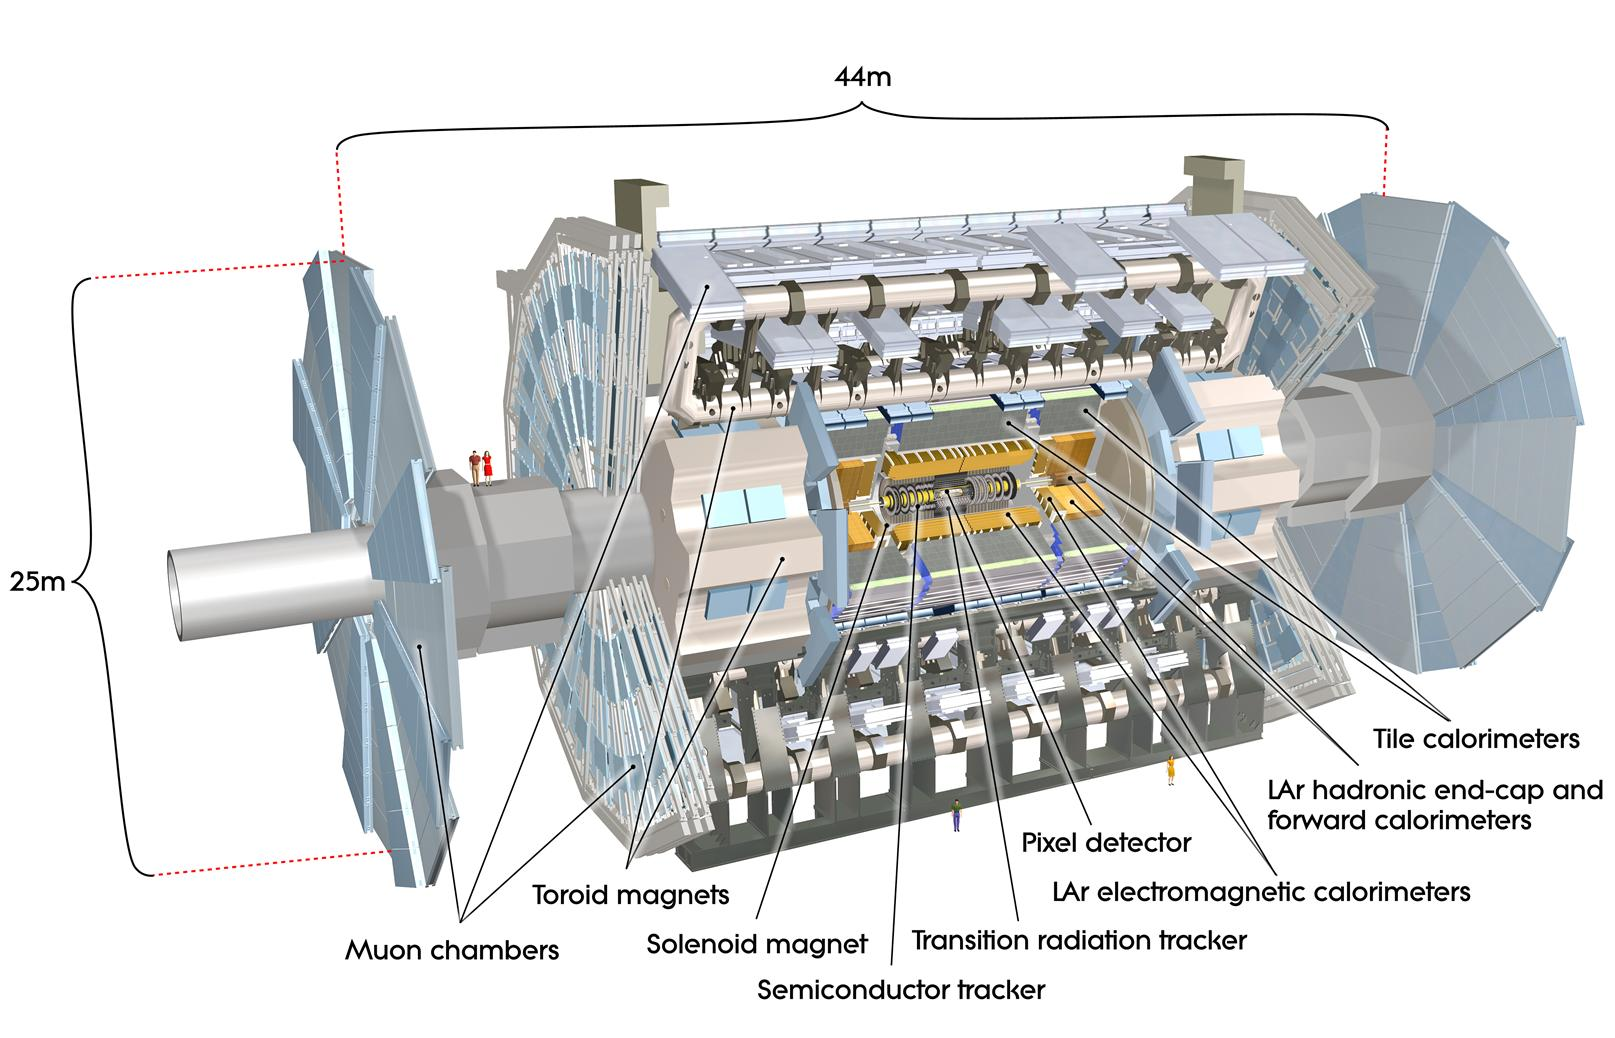
\includegraphics[width=\linewidth,height=\textheight,keepaspectratio]{atlas/atlas_xsec}
        \caption{Cutaway view of the ATLAS detector \cite{Pequenao:1095924}}
        \label{fig:atlas_xsec}
    \end{figure}

    % Purpose
    Core purpose is to accurately record the physical properties of the particle interactions which take place in the interaction region of the detector.
    Most of the particles of interest are extremely short-lived, and so their properties cannot be measured directly.
    Instead, we must detect the decay products of these particles, and reconstruct the original particles of interest after the fact.
    Accurate reconstruction of these original particles is critically dependant on measuring, as precisely as possible, the physical properties of the decay products.
    More specifically, ATLAS is designed to record the paths and decay showers of the particles which pass through the detector, in order to determine their mass, energy, momentum, and electric charge.

    % General barrel/endcap cylindrical structure
    In order to measure all the required properties, ATLAS is divided into many different subsystems.
    Each of these subsystems has a very different design and objective, but they are all constructed with roughly the same overall cylindrical geomtry.
    The reason for this design is simple kinematics.
    The LHC particle beams cross with no initial transverse momentum, which means particles are ejected without preference in the radial angle $\phi$.
    Furthermore, the extremely high longitudinal momentum of the beams results in many particles continuing along a highly "forward" (parallel to the beampipe) trajectory.
    These two properties lead naturally to a radially symmetric detector which is elongated in the forward direction; a cylinder centered on the beam axis.
    To accomodate this geometry, the various sub-detectors of ATLAS are generally split into two distinct parts, called "barrels" and "endcaps".
    The barrels are a series of radially symmetric cylindrical shells, concentric about the beampipes, meant to detect particles moving primarily in the transverse direction.
    Conversely, the endcaps are a series of flat, circular plates, stacked one behind the next along the beampipes, intended to detect more forward particles.

    \begin{figure}
        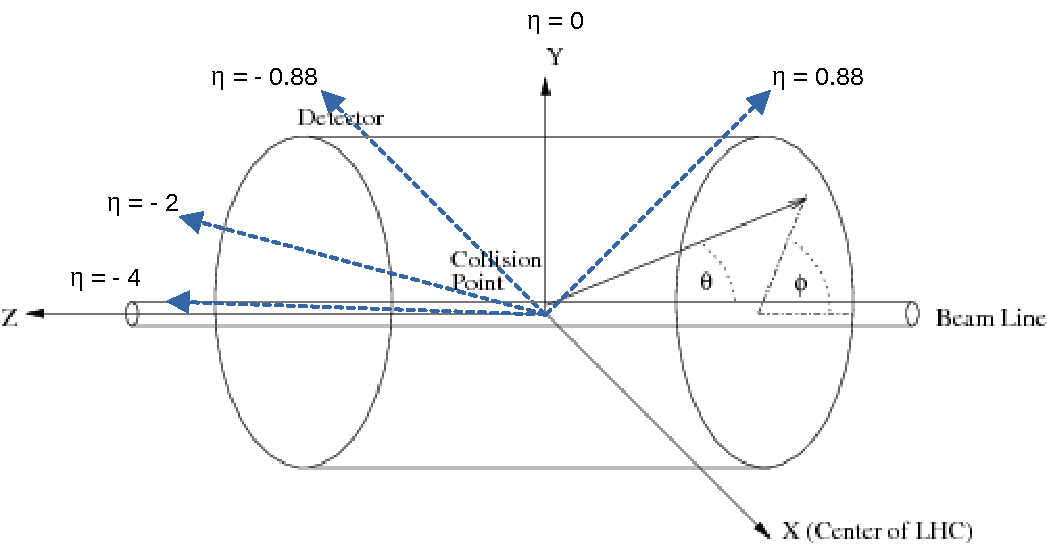
\includegraphics[width=\linewidth,height=\textheight,keepaspectratio]{atlas/atlas_coords}
        \caption{Illustration of the cylindrical coordinate system used in ATLAS \cite{Schott:1699952}}
        \label{fig:atlas_coords}
    \end{figure}

    % Walkthrough of the systems, from inner to outer, discussing why they are there and their basic purpose
    The various detector subsystems can be broken up into three primary groups, based on the subsystems' purpose.
    Moving out from the interaction region, the subsystems can be classified as belonging to the Inner Detector, the Calorimeters, or the Muon Spectrometer.
    The first of these, located as close in $r$ and $z$ as possible, is the Inner Detector system.
    The Inner Detector is desigined to provide momentum measurement, vertexing, and electron identification.
    It must be located so close to the interaction region in order to permit detection of short lived particles like b-quarks and tau leptons \cite{id_tdr}.
    Following immediately behind (endcap) and around (barrel) the Inner Detector is the collection of sensors comprising the Calorimetry system.
    These sensors are purpose-built to measure the energy of incoming particles and also provide supplementary tracking information for particle trajectories.
    Their location between the IR and Muon System is based on the fact that calorimeters function by absorbing all of a particle's energy, thereby stopping them.
    Since their function necessarily stops particles, they must be placed outside the range of the tracking system, as otherwise the trackers would never see particles.
    The Muon system however functions best when only muons traverse it, and so the calorimeters are intentionally placed between the IR and the Muon Spectrometer in order to shield the Muon system from unwanted hadrons.
    Finally, at the outer edge of ATLAS, is the Muon Spectrometer, which has been built to measure the momentum of muons leaving the detector volume.
    


% Then split off into sections for the individual subsystems


\section{Inner Detector} \label{sec:inner_detector}
    % Purpose of subsystem
    % Basic specs
    % What mechanism is used to achieve this purpose
    % What are the individual detectors and how do they contribute to this goal
    
    The Inner Detector system is intended to provide measurement of particles' momentum, provide vertex information, and help in identifying electrons.
    The way it achieves these goals is primarily through a series of very high resolution tracking sensors, which are used to trace out the paths that particles traverse as they leave the IR. 
    Momentum and charge measurement is facilitated by using a solenoid magnet to encompass the entire Inner Detector with a 2T axial magnetic field.
    This field bends the high-momentum charged particles into a helical trajectory, allowing their momentum, mass, and charge to be determined from the shape of the particle's path.
    The entire ID system, consisting of three independent detectors, measures 5.3 m in length and 2.5 m in diameter, and is able to provide accurate tracking within $|\eta| < 2.5$ \cite{id_tdr}.
    From the innermost to outermost, the sub-detectors are the Pixel Detector, the Semiconductor Tracker (SCT), and the Transition Radiation Tracker (TRT).
    The Pixel Detector and SCT together are responsible for high resolution tracking of particle trajectories.
    Further from the IR, the TRT provides more particle tracking capability at lower resolution (but higher statistics), as well the ability to help distinguish electrons. 

    \begin{figure}
        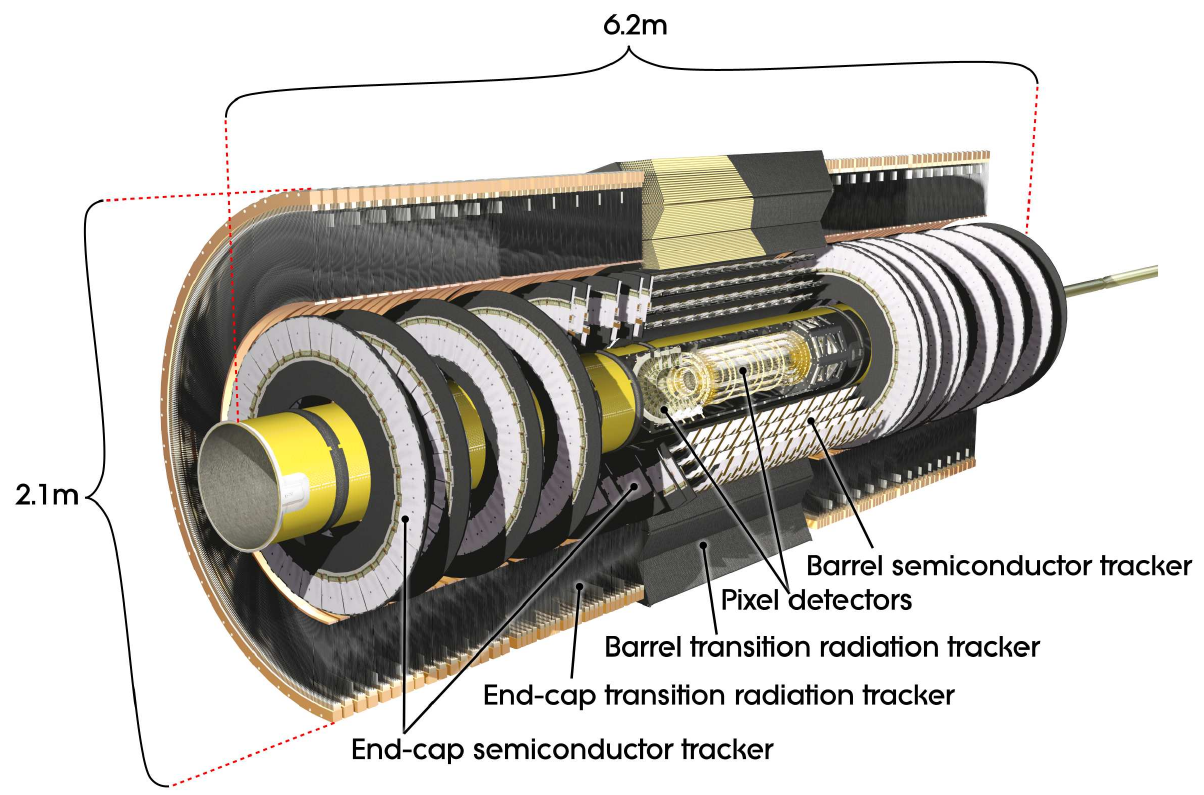
\includegraphics[width=\linewidth,height=\textheight,keepaspectratio]{atlas/inner_detector_xsec}
        \caption{Cutaway view of the Inner Detector sub-system \cite{atlas_tdr}}
        \label{fig:inner_detector_xsec}
    \end{figure}

    \begin{table} \centering
\caption{General specifications of Inner Detector modules \cite{atlas_tdr} \cite{insertable_Blayer}.}
\label{tab:ID_specs}
\begin{tabular}{ |l l|l|l| }
    \hline
    \textbf{Item}                   & &       \textbf{Radial extension (mm)} & \textbf{Length (mm)} \\
    \hline
    \textbf{Overall ID envelope}    & &         \textbf{0 < R < 1150}        &\textbf{0 < |z| < 3512} \\
    Beam-pipe                       & &            29 < R < 36    & \\
    \hline

    \textbf{IBL}          &  Overall envelope  &  31.0 < R < 40.0          &             \\    
                          &  Sensitive barrel  &  <R> = 25.7               &  |z| < 332 \\    
    &&&\\
    \textbf{Pixel}        &  Overall envelope  &  45.5 < R < 242           &  0 < |z| < 3092 \\
    3 cylindrical layers  &  Sensitive barrel  &  50.5 < R < 122.5         &  0 < |z| < 400.5 \\
    2 × 3 disks           &  Sensitive end-cap &  88.8 < R < 149.6         &  495 < |z| < 650 \\
    &&&\\
    \textbf{SCT}          &  Overall envelope  &  255 < R < 549 (barrel)   &  0 < |z| < 805 \\
                          &                    &  251 < R < 610 (end-cap)  &  810 < |z| < 2797 \\
    4 cylindrical layers  &  Sensitive barrel  &  299 < R < 514            &  0 < |z| < 749 \\
    2 × 9 disks           &  Sensitive end-cap &  275 < R < 560            &  839 < |z| < 2735 \\
    &&&\\
    \textbf{TRT}          &  Overall envelope  &  554 < R < 1082 (barrel)  &  0 < |z| < 780 \\
                          &                    &  617 < R < 1106 (end-cap) &  827 < |z| < 2744 \\
    73 straw planes       &  Sensitive barrel  &  563 < R < 1066           &  0 < |z| < 712 \\
    160 straw planes      &  Sensitive end-cap &  644 < R < 1004           &  848 < |z| < 2710 \\
    \hline
\end{tabular} \end{table}



    \subsection{Pixel Detector and Semiconductor Tracker}
        % purpose
        As the very first detector elements that any particles leaving the interaction region will encounter, the Pixel Detector and SCT face a precarious dilema.
        On the one hand, they must be able to accurately track the path of all ionizing particles emerging from the IR at high resolution (see table \ref{tab:ID_resolution}).
        On the other hand, any disturbance they introduce to particle trajectories will distort the measurment from every other detector in ATLAS.
        Add to this that these detectors face the highest radiation flux of any system simply by their proximity to the IR, forcing usage of very radiation-hard material design.
        For these reasons, the Pixel Detector and SCT use top-of-the-line silicon semiconductor diode technology, which can be made both extremely thin and sensitive. 
        This means that particles only deposit a small fraction of their energy into the detector material, and yet that small deposition is enough to accurately record their passage.
        With three layers of the Pixel Detector and four of the SCT, any particle leaving the IR crosses at least seven detector layers, yet continues on with a mostly unchanged trajectory.

        \begin{table}[] \centering \footnotesize
\caption{Resolution of the various Inner Detector Modules \cite{id_tdr}\cite{insertable_Blayer}.}
\label{tab:ID_resolution}
\begin{tabular}{|l|l|l|l|l|l|}
\hline
\textbf{System} & \textbf{Position} & \textbf{ Area }                 & \textbf{ Resolution }   & \textbf{ Channels } & \textbf{$\eta$} \\
\textbf{}       & \textbf{        } & \textbf{(m\textsuperscript{2})} & \textbf{\sigma($\mu$m)} & \textbf{ ($10^6$) } & \textbf{Coverage} \\
\hline
Pixels         & 1 insertable barrel layer & 0.38      & $R\phi$ = 50, z = 250    & 13.2           & $\pm 3  $       \\
               & 1 removable barrel layer  & 0.2       & $R\phi$ = 12, z = 66     & 16             & $\pm 2.5$       \\
               & 2 barrel layers           & 1.4       & $R\phi$ = 12, z = 66     & 81             & $\pm 1.7$       \\
               & 4 end-cap disks           & 0.7       & $R\phi$ = 12, R = 77     & 43             & 1.7-2.5         \\
               & on each side              &           &                          &                &                 \\
Silicon strips & 4 barrel layers           & 34.4      & $R\phi$ = 16, z = 580    & 3.2            & $\pm 1.4$       \\
               & 9 end-cap wheels          & 26.7      & $R\phi$ = 16, R = 580    & 3.0            & 1.4–2.5         \\
               & on each side              &           &                          &                &                 \\
TRT            & Axial barrel straws       &           & 170 (per straw)          & 0.1            & $\pm 0.7$       \\
               & Radial end-cap straws     &           & 170 (per straw)          & 0.32           & 0.7–2.5         \\
               & 36 straws per track       &           &                          &                &                 \\
\hline
\end{tabular} \end{table}


        Semiconductor diode detectors function by exploiting the properties of semiconductor p-n junctions.
        These particular detectors are made using silicon.
        Silicon has four valence electrons, so a pure silicon crystal lattice will have its valence band perfectly filled, leading to a very stable structure.
        A pure semiconductor crystal lattice (in this case, silicon) can have impurities intentionally introduced to it through the process of doping.
        Doping the lattice with an element possesing only three valence electrons (e.g. Boron) will result in a number of gaps in the valence band (called "holes").
        In such a situation, known as p-type doping, the lattice will accept additional electrons to fill these holes, which will lead to an excess of negatively charged ions.
        Conversly, an element with five valence electrons can be introduced for doping, leading to an excess of electrons in the valence band.
        Known as n-type doping, such an excess results in a lattice with a propensity for shedding these excess valence electrons, which in turn leads to an excess of positive ions.
        A p-n junction can be produced by taking a single silicon wafer and n-type doping one half, while p-type doping the other.
        The junction where the two dopings meet will then see a transfer of excess valence electrons moving from the n-type side to fill the holes of the p-type side, as illustrated in figure \ref{fig:pn_junction}

        \begin{figure}
            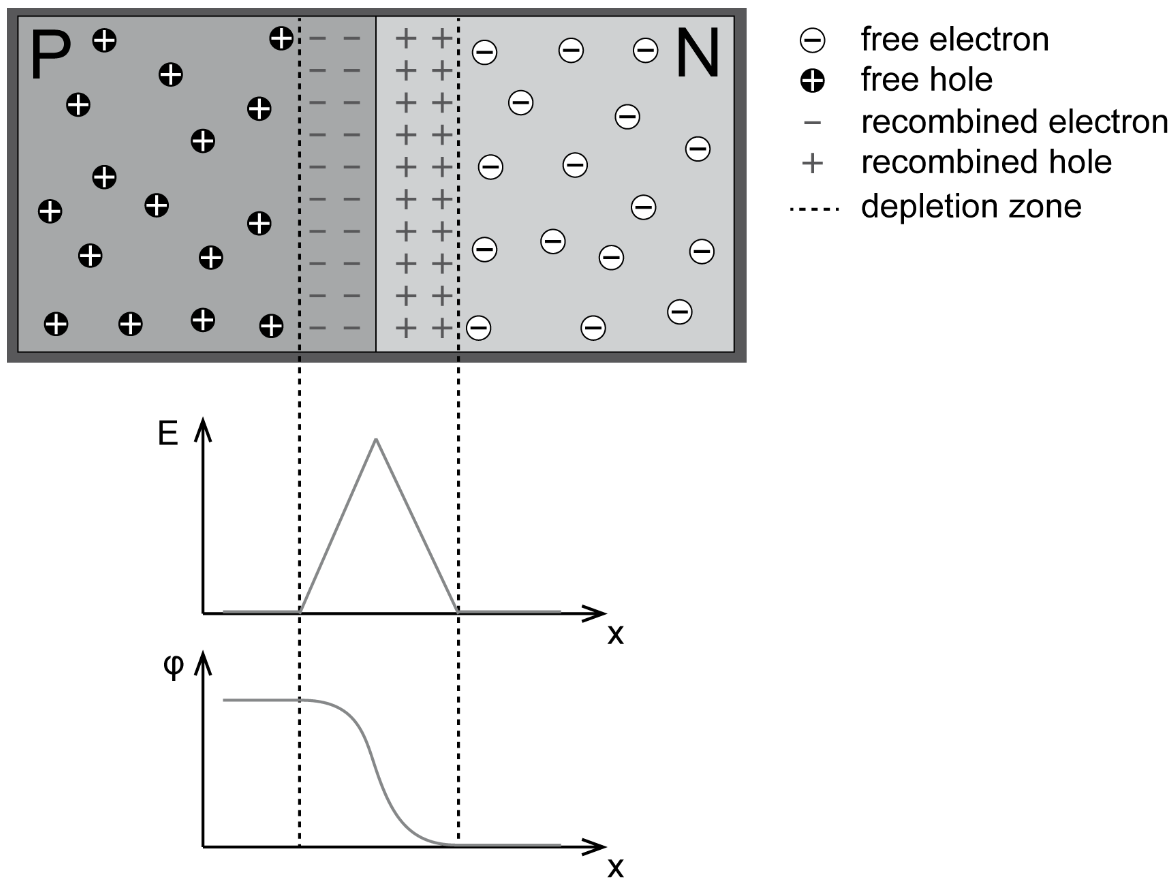
\includegraphics[width=\linewidth,height=\textheight,keepaspectratio]{atlas/pn_junction}
            \caption{Representation of a p-n junction, its depletion region, and the electric field and potential across its surface \cite{Havránek:2317324}}
            \label{fig:pn_junction}
        \end{figure}

        As the excess "donor" electrons migrate to fill the "acceptor" holes, the area around the junction has its valence band filled, creating an area called the "depletion zone".
        Though the depletion zone has a filled valence band, it has done so at the cost of ionization; an excess of electrons now populates the p-type side, with an equal number of positive ions remaining on the n-type side.
        The depletion zone grows larger until the migration of holes and electrons is balanced by the electric potential created through this ionization.
        When equilibrium is achieved, the lattice is left with an electric potential which monotonically decreases from the n-type to the p-type side, and which spans the full width of the depletion zone (refer again to figure \ref{fig:pn_junction}).
        If a voltage is applide across the semiconductor, the width and potential difference of the depletion region can be altered.
        If the voltage is applied with the positive end of the difference at the p-type side, then the semiconductor is said to be "forward biased", and the depletion region will become smaller (and with a high enough voltage can be eliminated entirely).
        If the positive end of the voltage difference is applied to the n-type side though, the semiconductor becomes "reverse biased", and the depletion region and potential difference across the junction will grow larger \cite{wiley_radiation_detection}.
        In this reverse-biased state, the electric potential of the p-n junction becomes very effective at rapidly sweeping excess ions from the depletion region off to the edges of the semiconductor wafer, and it is this mechanism which the ATLAS semiconductor detectors exploit in order to detect particles.

        Ionizing radiation is any particle that interacts electromagnetically, which means either photons or any particle with electric charge.
        When ionizing radiation passes through an element of the Pixel Detector or SCT, it will momentarily separate electrons from their nuclei in the silicon lattice.
        Normally, such separated ions would just recombine in a matter of moments.
        Because of the electric potential in the depletion region though, these ions are further seperated, and swiftly arrive at opposite ends of the semiconductor wafer.
        The very leads responsible for biasing the semiconductor are then responsible for collecting these seperated ions, which will cause a sudden jump in the circuit's current.
        The electric current through these semiconductor detectors is closely monitored, and these spikes are used to identify the passage of a particle through the semiconductors.

    \subsection{Transition Radiation Tracker (TRT)}
            Where the Pixel Detector and SCT focus on quality over quantity in their tracking, the TRT serves to take the opposite approach.
            The TRT has a resolution much lower than that of either the Pixel or SCT.
            But where the Pixel and SCT combined only manage about seven recorded hits per particle, the TRT achieves around 36.
            High statistics then are able to offset the TRT's lower resolution per hit, overall achieving a similar uncertainty on its track measurments.
            Such measurement needs to be accomplished under the same restrictions faced by the earlier trackers though.
            Namely, that it must obtain these measurements while causing minimal deviation in particle trajectory and also tolerating heavy radiation exposure over time.
            These challenges and goals are addressed in the TRT's composition, using a detector technology known as ``proportional drift tubes".

            The TRT consists of a large number of proportional drift tubes, often referred to as ``straws".
            Proportional drift tubes function in a similar way to semiconductor diode detectors, but using a gas instead of a doped semiconductor.
            The primary component of a drift tube is a cylinder filled with a gas mixture.
            In the TRT, these cylinders are 4 mm in diameter, filled with a mixture of 70\% Xenon, 27\%CO\textsuperscript{2}, and 3\% O\textsuperscript{2}.
            Ions are produced in this mixture when ionizing radiation passes through it.
            As in the semiconductor diode detectors, these ions are collected by applying an electric field through the ionization medium in order to sweep ions away into external circutry for readout.
            In a drift tube this is accomplished by maintaining an electric potential between the tube wall and a conductive wire running through the cylinder axis \cite{drift_chambers}.
            %NOTE: do I need to mention avalanche multiplication?
            The wall of the tube acts as the positively charged anode to collect electrons produced by the ionization, while the axial wire is kept at high electrical potential to act as the cathode.
            In the TRT, the cathode wall is made of aluminium and the 30 $\mu$m diameter anode wire of gold-plated tungsten. \cite{trt_design}

            \begin{figure}
                \begin{subfigure}{.48\textwidth}
                    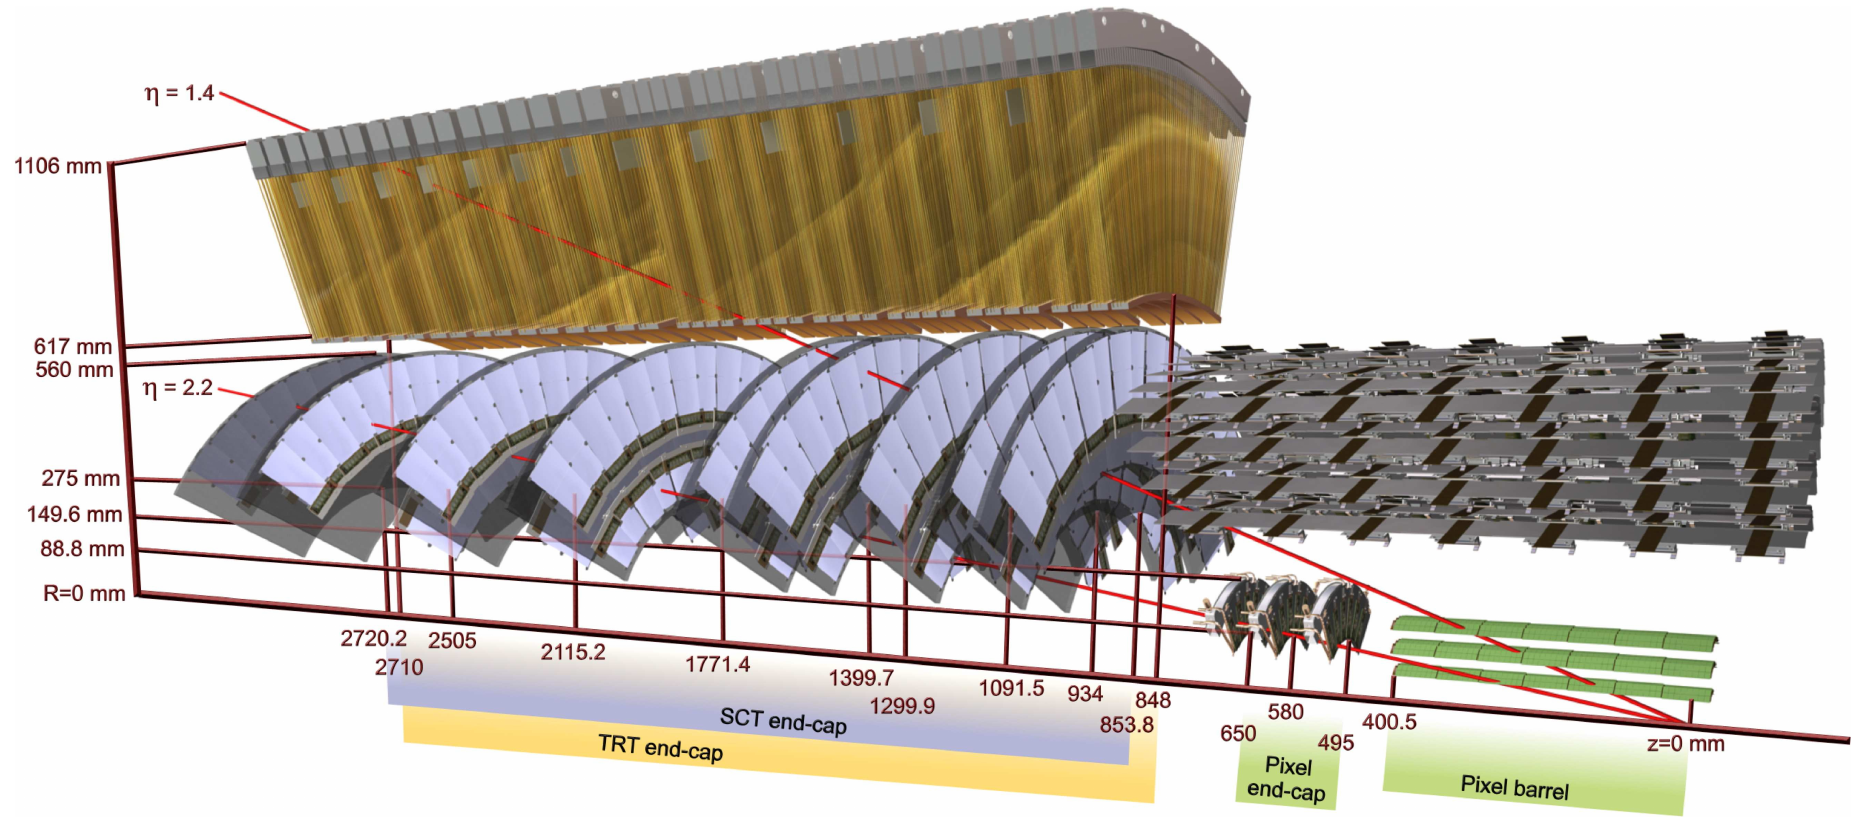
\includegraphics[width=\linewidth,height=\textheight,keepaspectratio]{atlas/inner_detector_endcap_measurements}
                    \caption{ID Endcap}
                    \label{fig:inner_detector_endcap_measurements}
                \end{subfigure}
                \begin{subfigure}{.48\textwidth}
                    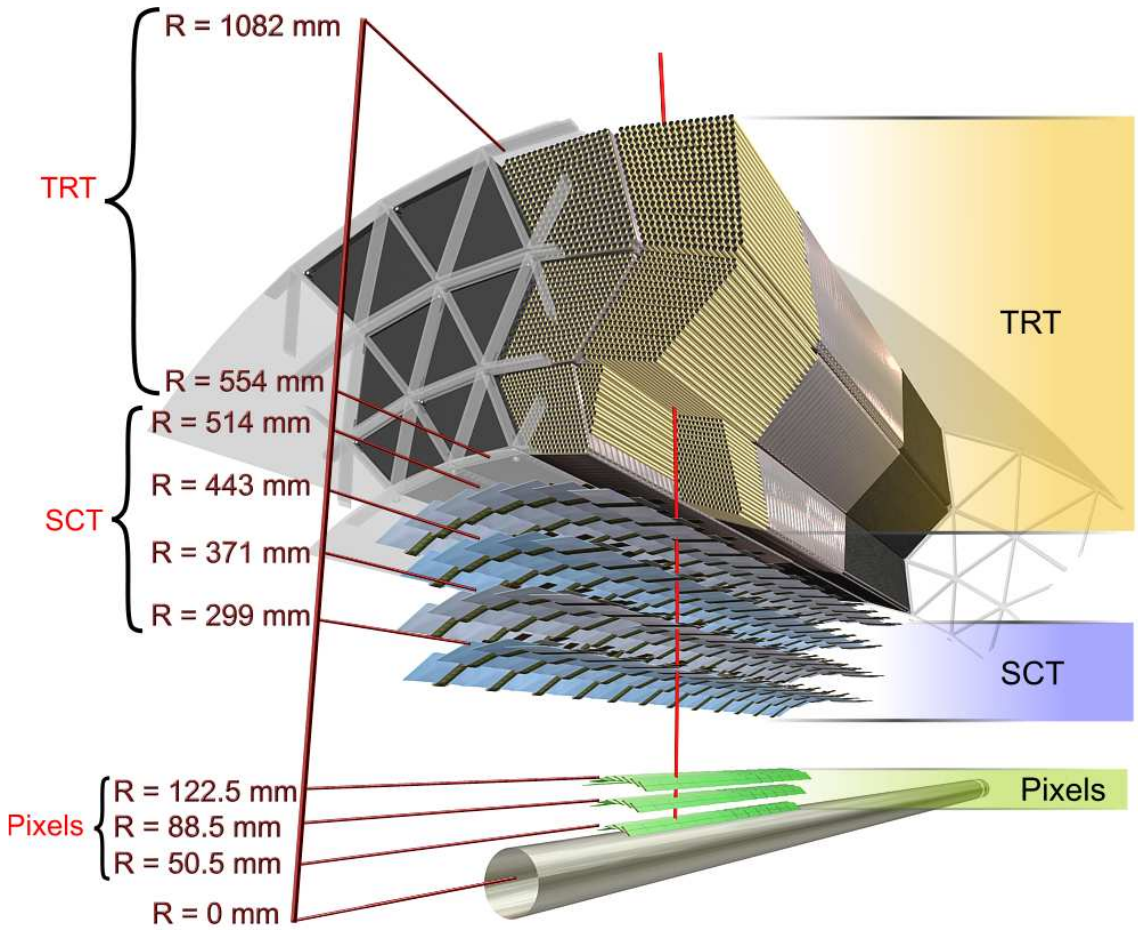
\includegraphics[width=\linewidth,height=\textheight,keepaspectratio]{atlas/inner_detector_barrel_measurements}
                    \caption{ID Barrel}
                    \label{fig:inner_detector_barrel_measurements}
                \end{subfigure}
                \caption{Visualization of the Inner Detector modules with corresponding measurments \cite{atlas_tdr}}
                \label{fig:inner_detector_measurements}
            \end{figure}

            For the TRT barrel, there are 52,544 straws 144 cm in length, while the endcaps each contain 122,880 straws 37 cm in length.
            These straws are arranged parallel to the beampipe in the barrel, and orthogonal to the beampipe in the endcap (see figure \ref{fig:inner_detector_measurements}).
            This arrangment is to maximize the number of straws traversed by an outgoing particle, typically 35-40 straws for $0 < |\eta| < 2$.
            Though each individual hit has a relatively low spatial resolution compared to the semiconductor detectors, the large number of hits compensates for this with a reduced statistical uncertainty.

            In addition to providing additional tracking information, the TRT provides a secondary purpose of aiding in the identification of electrons by means of detecting transition radiation. 
            Transition radiation is a phenomenon in which radiation is emitted when a charged particle crosses a boundary between two materials \cite{transition_radiation}.
            The TRT uses polypropylene as its transition radiation material, which is interleaved between the layers of straws.
            In the barrel, there are 73 layers of straws interwoven with polypropylene fibres, and in the endcaps there are 160 layers of straws with polypropylene foil between them.
            The large number of layers provide ample and repeated oppurtunity for charged particles crossing the TRT to encounter transition layers and emit identifying radiation, which is later used to distinguish electrons from other ionizing radiation.


\section{Calorimetry} \label{sec:calorimeter}
    The ATLAS Calorimeter system is designed to measure the energy of particles emerging from the Interaction Region.
    The entire collection of sub-detectors extends from the immediate outer edge of the Inner Detector region, out to a radius of 4.25 m, and longitudinally out to 6.12 m.
    Together the various systems achieve complete measurment coverage out to $|\eta| < 4.9$.

    There are a number of different ways to measure the energy of a particle, but in ATLAS this is done exclusively using the class of calorimeters known as \textit{sampling} calorimeters.
    Fundamentally, particle calorimeters work by impeding the path of a particle with some material, such that the particle is forced to interact with that material and deposit energy into it.
    This interaction must be such that it produces a measurable response, proportional to the deposited energy.
    A sampling calorimeter functions by measuring only a fraction of the deposited energy, spread out across the detector medium; i.e. by taking a sample of the energy.
    To do this, two different materials are used in the detector's construction, reffered to as the active and inactive materials.
    The active material is the material which actually measures the energy of particles, using the same or similar techniques as the tracking systems discussed earlier.
    The inactive material in turn has no detection capababilities, but is instead meant purely for the purpose of the aforementioned impedence of particle trajectories.
    Typically, inactive calorimeter material is a very dense and heavy high $Z$ medium, in order to maximize the number of particle interactions per unit distance.
    The active and inactive materials are arranged in alternating layers, so that the active material gets a snapshot of the way the particle is depositing energy across the entire length of the detector.\cite{energy_measurement}

    \begin{figure}
        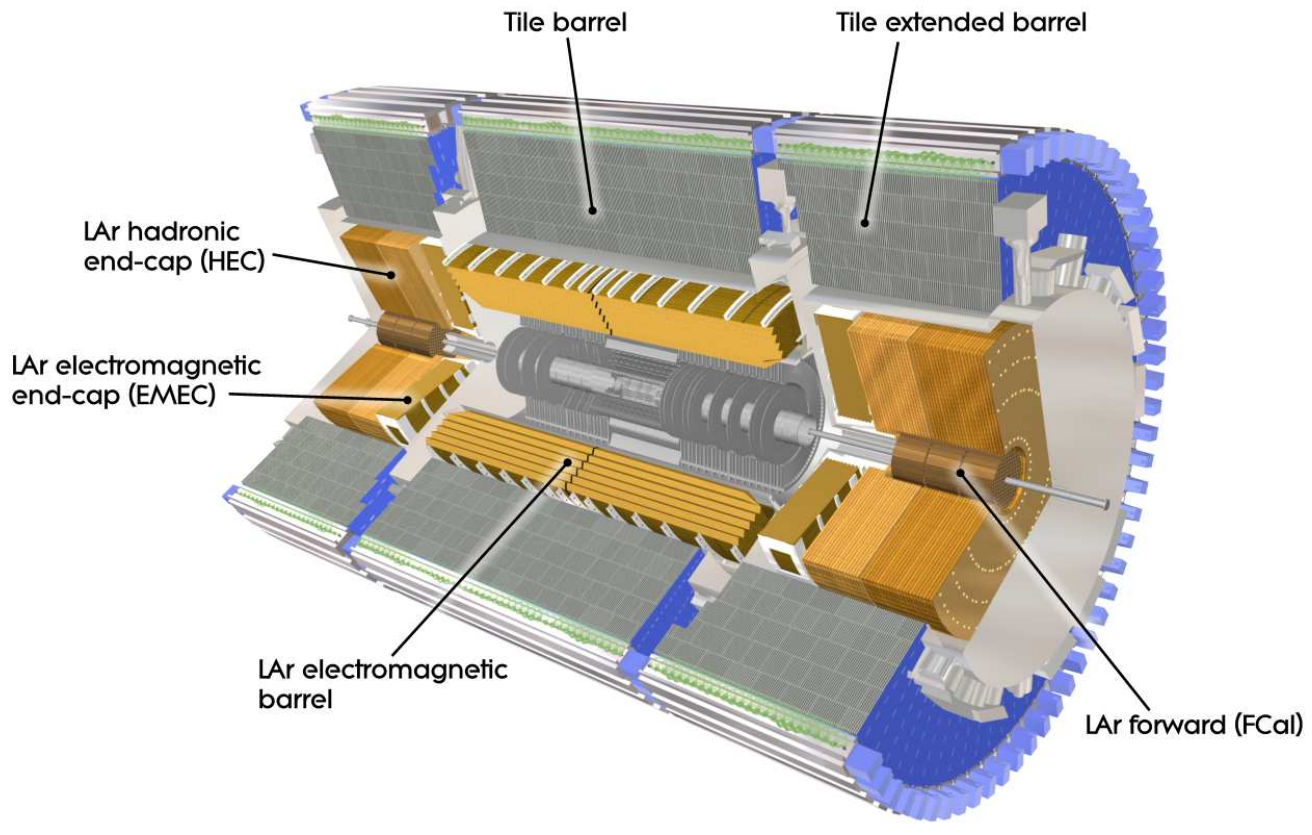
\includegraphics[width=\linewidth,height=\textheight,keepaspectratio]{atlas/cal_xsec}
        \caption{Cutaway view of the Calorimetry sub-system \cite{atlas_tdr}}
        \label{fig:cal_xsec}
    \end{figure}

    The Calorimetry system is split among three different subsystems, designed to measure two distinct kinds of particles.
    The innermost of these subsystems is the Electromagnetic Calorimeter (ECal), designed primarily to measure (anti) electrons and photons \cite{calorimetry_lecture}.
    These particles readily interact electromagnetically in the calorimeter material, rapidly losing energy and permitting the ECal to be more compact.
    Surrounding the ECal are the Hadronic Calorimeter (HCal) systems.
    These detectors, as their name suggests, detect hadrons, such as neutrons or pions.
    Not only are these particles heavier, but many of them are electrically neutral and can therefore only be stopped through repeated nuclear interactions \cite{energy_measurement}.
    Consequently, the HCal systems are significantly thicker and use more dense inactive materials that that of the ECal (see figure \ref{fig:cal_rad_length}).
    \begin{figure}
        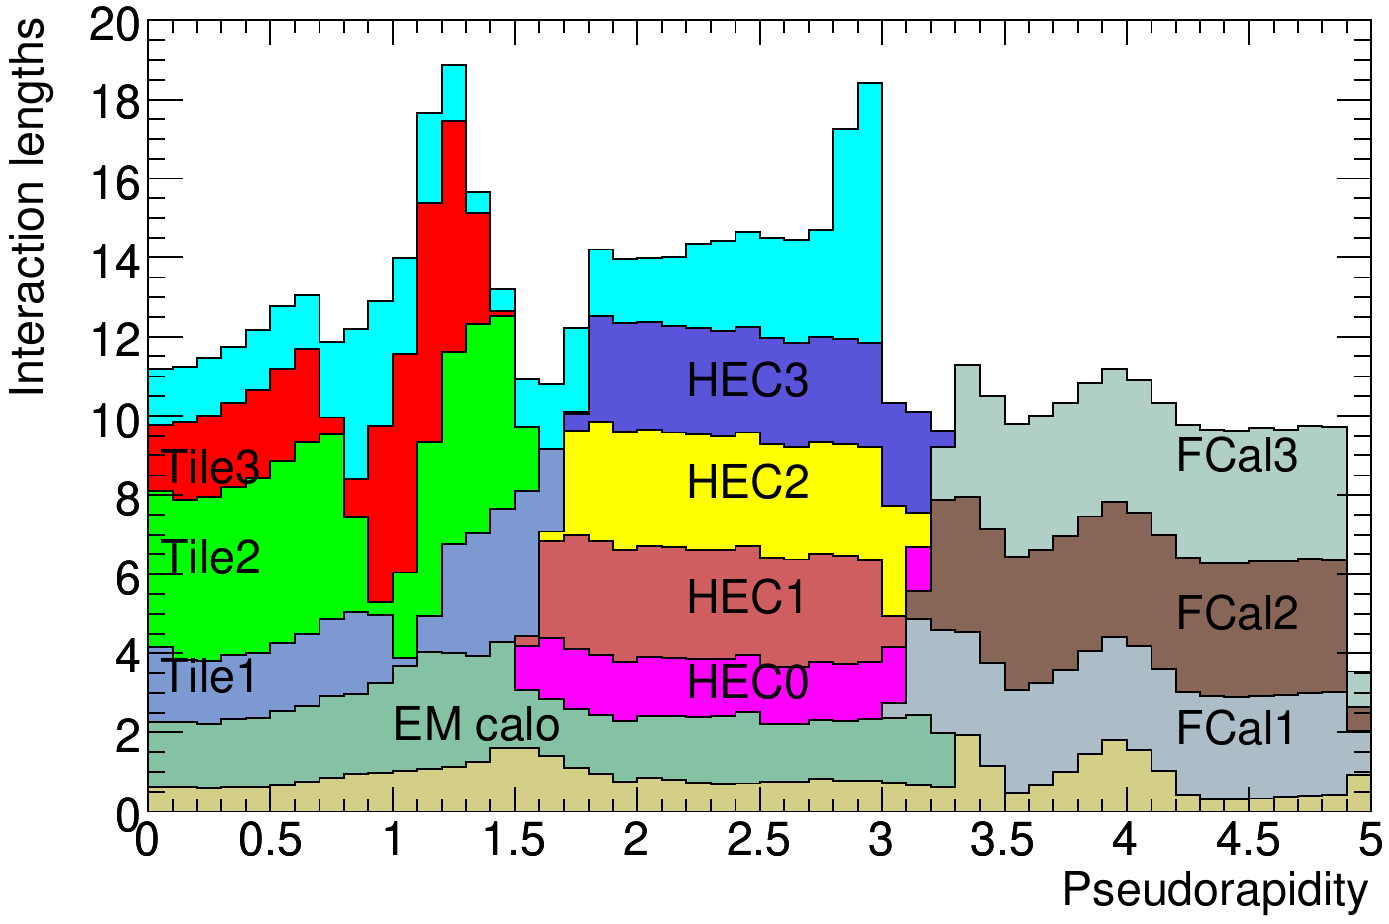
\includegraphics[width=\linewidth,height=\textheight,keepaspectratio]{atlas/cal_rad_length}
        \caption{Histogram of interaction lengths $X_0$ as a function of $\eta$ for the different sub-detectors \cite{atlas_tdr}}
        \label{fig:cal_rad_length}
    \end{figure}
    Additionally, they serve the crucial role of preventing hadrons from escaping into the Muon Spectrometer.
    The final subsystem of the Calorimetry system is the Forward Calorimeter (FCal).
    The FCal records, across different sections, the energy of electromagnetic and hadronic particles.
    It is constructed very close to the beampipe, and serves to extend the calorimetric measurement coverage out to an $|\eta|$ of 4.9.

    \subsection{Electromagnetic Calorimeters}
        Purpose is to detect electrons and photons at high resolution.
        Both barrel and encaps use lead as their inactive material, and Liquid Argon as the active material.
        The liquid argon calorimeters, used in the ECal and elsewhere, detects ionization from incident particles via capacitive coupling to electrodes placed outside the active medium.
        Liquid argon as the active medium in particular is used because of its intrinsic radiation hardness and linear ionization response to radiation \cite{Lar_cal_tdr}.
        Uses a unique "accordian" design in the layout of the material layers, in order to provide complete coverage in $\phi$.
        Also uses a "Presampler", due to an excess of material in front of the ecal.
        Presampler needed to account for energy lost in this material


    \subsection{Hadronic Calorimeter}
        Serves to detect hadrons, and to prevent "punch-through" into the Muon System.
        The Hadronic Endcap Calorimeter (HEC) uses Liquid Argon for the active material, like the ECals, but uses copper plates for the inactive material.
        The HCal Barrel, referred to as the Tile Calorimeter, uses steel plates as the inactive material, and scintillating tiles as the active material.
        The scintillating tiles used here operate on different electrical principles than the LAr detectors used across the other calorimeters.
        The key to scintillating materials is that they respond to ionizaing radiation by fluorescing.
        That is, when ionizing radiation crosses through the scintillation material, the material momentarily enters an excited state.
        The excited material promptly returns to its base energy state, and releases the excess energy in the form of photons, called "scintillation light".
        Ideally, this flourescent response is related to the energy of the incident radiation through as linear a response as possible \cite{wiley_radiation_detection}.
        In the Tile Calorimeter, the scintillating material used is polystyrene, and the energy itself is measured by transferring the light to optical fibres located at the edge of the tile modules.
        These optical fibres direct the light to photomultiplier tubes (PMTs), which in turn convert the light to electrical signals to be read out \cite{tcal_tdr}.


    \subsection{Forward Calorimeter}
        Purpose is to extend calorimetry coverage as far as $|\eta| < 4.9$.
        Divided into three parts: 1 ECal, and 2 HCals
        All parts use LAr for active medium, but ECal uses copper while Hcals use Tungsten for inactive medium
        Exposed to extremely high radiation flux, necessitating materials that are both very dense and very radiation-resistant \cite{Lar_cal_tdr}.

    \begin{table}[] \tiny \centering
\caption{General specifications of calorimeter systems \cite{atlas_tdr}.}
\label{tab:cal_specs}
\begin{tabular}{|l|lc|lc|}
\hline 
                                               &                  \multicolumn{2}{c|}{\textbf{Barrel}}            &           \multicolumn{2}{c|}{\textbf{End-cap}}                                 \\
\hline 
                                               \multicolumn{5}{|c|}{\textbf{EM Calorimeter}} \\
\hline 
                                               \multicolumn{5}{|c|}{Number of layers and $|\eta|$ coverage} \\
\hline 
Presampler                                     & 1                 & $|\eta|$ < 1.52                 & 1                               & 1.5 < $|\eta|$ < 1.8     \\
Calorimeter                                    & 3                 & $|\eta|$ < 1.35                 & 2                               & 1.375 < $|\eta|$ < 1.5   \\
                                               & 2                 & 1.35 < $|\eta|$ < 1.475 & 3                                       & 1.5 < $|\eta|$ < 2.5     \\
                                               &                   &                                 & 2                            & 2.5 < $|\eta|$ < 3.2     \\
\hline 
                                               \multicolumn{5}{|c|}{Granularity $\Delta \eta \times \Delta \phi$ versus $|\eta|$} \\
\hline 
Presampler                                     & 0.025 × 0.1       & $|\eta|$ < 1.52                 & 0.025 × 0.1                     & 1.5 < $|\eta|$ < 1.8     \\
Calorimeter 1st layer                          & 0.025/8 × 0.1     & $|\eta|$ < 1.40                 & 0.050 × 0.1                     & 1.375 < $|\eta|$ < 1.425 \\
                                               & 0.025 × 0.025     & 1.40 < $|\eta|$ < 1.475 & 0.025 × 0.1                             & 1.425 < $|\eta|$ < 1.5   \\
                                               &                   &                                    & 0.025/8 × 0.1                   & 1.5 < $|\eta|$ < 1.8     \\
                                               &                   &                                    & 0.025/6 × 0.1                   & 1.8 < $|\eta|$ < 2.0     \\
                                               &                   &                                    & 0.025/4 × 0.1                   & 2.0 < $|\eta|$ < 2.4     \\
                                               &                   &                                    & 0.025 × 0.1                     & 2.4 < $|\eta|$ < 2.5     \\
                                               &                   &                                    & 0.1 × 0.1                       & 2.5 < $|\eta|$ < 3.2     \\
\hline 
Calorimeter 2nd layer                          & 0.025 × 0.025     & $|\eta|$ < 1.40                    & 0.050 × 0.025                   & 1.375 < $|\eta|$ < 1.425 \\
                                               & 0.075 × 0.025     & 1.40 < $|\eta|$ < 1.475 & 0.025 × 0.025                              & 1.425 < $|\eta|$ < 2.5   \\
                                               &                   &                                    & 0.1 × 0.1                       & 2.5 < $|\eta|$ < 3.2     \\
\hline 
Calorimeter 3rd layer                          & 0.050 × 0.025     & $|\eta|$ < 1.35                 & 0.050 × 0.025                   & 1.5 < $|\eta|$ < 2.5     \\
\hline 
                                               \multicolumn{5}{|c|}{Number of readout channels} \\
\hline 
Presampler                                     & 7808              &                                    & 1536 (both sides)               &                                     \\
Calorimeter                                    & 101760            &                                    & 62208 (both sides)              &                                     \\
\hline 
                                               \multicolumn{5}{|c|}{\textbf{LAr Hadronic End-cap}} \\
\hline 
$|\eta|$ coverage                              &                   &                                    & 1.5 < $|\eta|$ < 3.2 &                                     \\
Number of layers                               &                   &                                    & 4                               &                                     \\
\hline 
Granularity $\Delta \eta \times \Delta \phi$   &                   &                                    & 0.1 × 0.1                       & 1.5 < $|\eta|$ < 2.5     \\
                                               &                   &                                    & 0.2 × 0.2                       & 2.5 < $|\eta|$ < 3.2     \\
\hline 
Readout channels                               &                   &                                    & 5632 (both sides)               &                                     \\
\hline 
                                                       \multicolumn{5}{|c|}{\textbf{LAr Forward Calorimeter}} \\
\hline 
$|\eta|$ coverage                              &                   &                                    & 3.1 < $|\eta|$ < 4.9 &                                     \\
Number of layers                               &                   &                                    & 3                               &                                     \\
\hline 
Granularity $\Delta x \times \Delta y$ (cm)    &                   &                                    & FCal1: 3.0 × 2.6                & 3.15 < $|\eta|$ < 4.30   \\
                                               &                   &                                    & FCal1: \~ four times finer       & 3.10 < $|\eta|$ < 3.15,  \\
                                               &                   &                                    &                                 & 4.30 < $|\eta|$ < 4.83   \\
                                               &                   &                                    & FCal2: 3.3 × 4.2                & 3.24 < $|\eta|$ < 4.50   \\
                                               &                   &                                    & FCal2: \~ four times finer       & 3.20 < $|\eta|$ < 3.24,  \\
                                               &                   &                                    &                                 & 4.50 < $|\eta|$ < 4.81   \\
                                               &                   &                                    & FCal3: 5.4 × 4.7                & 3.32 < $|\eta|$ < 4.60   \\
                                               &                   &                                    & FCal3: \~ four times finer       & 3.29 < $|\eta|$ < 3.32,  \\
                                               &                   &                                    &                                 & 4.60 < $|\eta|$ < 4.75   \\
\hline 
Readout channels                               &                   &                                    & 3524 (both sides)               &                                     \\
\hline 
                                               \multicolumn{5}{|c|}{\textbf{Scintillator Tile Calorimeter}} \\
\hline 
                                               & Barrel            &                                    & Extended barrel                 &                                     \\
\hline 
$|\eta|$ coverage                              &    $|\eta|$ < 1.0 &                                    & 0.8 < $|\eta|$ < 1.7 &                                     \\
Number of layers                               & 3                 &                                    & 3                               &                                     \\
\hline 
Granularity $\Delta \eta \times \Delta \phi$   & 0.1 × 0.1         &                                    & 0.1 × 0.1                       &                                     \\
Last layer                                     & 0.2 × 0.1         &                                    & 0.2 × 0.1                       &                                     \\
\hline 
Readout channels                               & 5760              &                                    & 4092 (both sides)               &                                    \\
\hline 
\end{tabular} \end{table}




\section{Muon Spectrometer} \label{sec:muon}
    The Muon Spectrometer has the purpose of providing track position and momentum measurements for muons exiting the ATLAS detector.
    The Muon barrels start at a radii of 5 m from the beam axis, extending out to 10 m.
    The endcaps start at a $|z|$ of roughly 7.4 m, and proceed to an extent of 21.5 m.
    The immense size of the muon system poses a challenge, as it must provide tracking across its entire volume.
    %Its distance from the interaction point ameliorates this issue though, as it permits the Muon detectors to operate at much lower spatial resultions than the inner detectors, while still retaining similar anngular resolution.

    \begin{figure}
        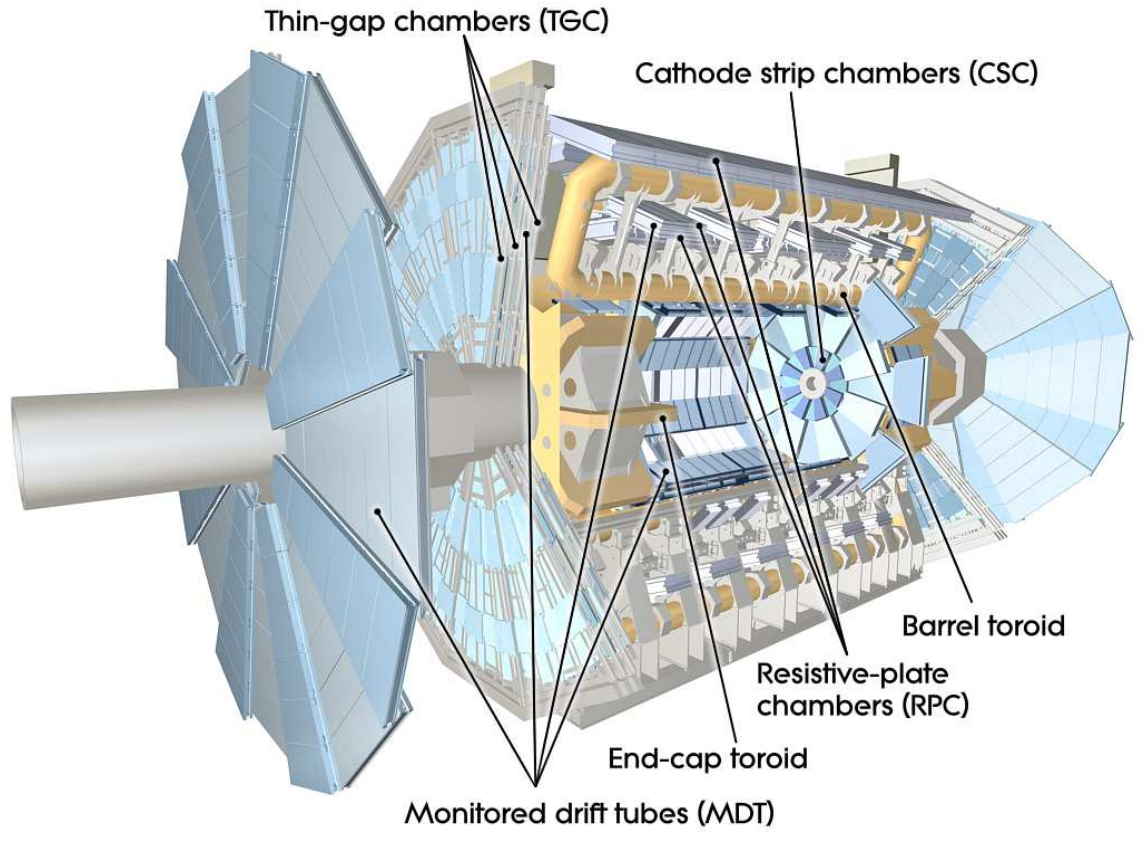
\includegraphics[width=\linewidth,height=\textheight,keepaspectratio]{atlas/muon_xsec}
        \caption{Cutaway view of the Muon Spectrometer \cite{atlas_tdr}}
        \label{fig:muon_xsec}
    \end{figure}

    \subsection{Toroid magnets}
        Three large air-core toroids meant to deflect muons.
        Barrel provides 1.5-5.5 Tm (Tesla-meters???) of bending power in $0<|\eta|<1.4$,
        and endcaps provide 1-7.5 Tm in $1.6<|\eta|<2.7$.
        The power is lower in the region where the fields overlap ($1.4<|\eta|<1.6$)

    \subsection{Precision Track Chambers}
        The Precision Track Chambers are designed to provide high resolution measurements of track position and momentum for particles escaping the ATLAS detector. Split across two technologies, the Monitored Drift Tube Chambers (MDT's) and Cathode-Strip Chambers (CSC's).
        The MDT's are drift tube chambers (like the earlier TRT, but larger) filled with Ar/CO2 gas using a tungsten-rhenium wire for charge collection. These are used in both the barrel and endcap regions, covering the range $|\eta| < 2.7$.
        The MDT consists of three endcap and three barrel layers, with a notable exception in the endcap region $2 < |\eta| < 2.7$.
        Within this $\eta$ range, for the first layer, the muon track density exceeds the resolution capabilities of the MDT's.
        As such, the first layer of the endcap in this range is replaced with CSC's.
        The CSC's are multiwire drift chambers, meaning that the (gold-plated tungsten) anode wires do not each have their own individual drift tube.
        Instead, each of the many drift chambers containes many anodes and many cathode strips, made of copper.
        These chambers can read both coordinates of a track simultaneosly, preventing the ambiguities that can occur if more than one track is present in the same chamber \cite{atlas_tdr}.

    \subsection{Trigger Chambers}
        Meant to provide rapid information on muon track multiplicity and energy range.
        Also provides additional track information for higher level triggers.
        Provides acceptance in range $|\eta| < 2.4$.
        The barrel and end-cap use two different technologies in order to address the different issues present in their respective regions.
        The barrel uses Resistive Plate Chambers (RPC's), which have higher temporal resolution.
        RPC's follow the same principle of operation as drift tube chambers, but the anode and cathodes are both conductive plates that maintain an electric potential in the gaseous mixture between them.
        The endcap consists of Thin Gap Chambers (TGC's), which are multi-wire drift tube chambers with very small gaps between the anode wires and the cathode strips; indeed, the anode-cathode gaps are 1.4 mm are smaller than the anode-anode gaps of 1.8 mm.
        The TGC serves to both tag beam-crossings and also deliver additional information on traversing particles' azimuthal coordinate, to complement the measurments of the MDT.

    \begin{table}[hb] \centering \scriptsize
\caption{General specifications of the Muon Spectrometer \cite{atlas_tdr}.}
\label{tab:muon_specs}
\begin{tabular}{|l|l|}
\hline
\textbf{Monitored Drift Tubes}    & \textbf{MDT}                                                      \\
- Coverage               & $|\eta|$ < 2.7 (innermost layer: $|\eta|$ < 2.0)         \\
- Number of chambers     & 1088 (1150)                                              \\
- Number of channels     & 339 000 (354 000)                                        \\
- Function               & Precision tracking                                       \\
\hline
\textbf{Cathode Strip Chambers}   & \textbf{CSC}                                                      \\
- Coverage               & 2.0 < $|\eta|$ < 2.7                                     \\
- Number of chambers     & 32                                                       \\
- Number of channels     & 31 000                                                   \\
- Function               & Precision tracking                                       \\
\hline
\textbf{Resistive Plate Chambers} & \textbf{RPC}                                                      \\
- Coverage               & $|\eta|$ < 1.05                                          \\
- Number of chambers     & 544 (606)                                                \\
- Number of channels     & 359 000 (373 000)                                        \\
- Function               & Triggering, second coordinate                            \\
\hline
\textbf{Thin Gap Chambers}        & \textbf{TGC}                                                      \\
- Coverage               & 1.05 < $|\eta|$ < 2.7 (2.4 for triggering)               \\
- Number of chambers     & 3588                                                     \\
- Number of channels     & 318 000                                                  \\
- Function               & Triggering, second coordinate                            \\
\hline
\end{tabular} \end{table}



% Ch5: Data - DRAFT 1.5
\chapter{Data Collection and Simulation} \label{chapter:data}

\section{Introduction}
    
    ATLAS is responsible for collecting all the experimental data required for this analysis,
        but that data is of limited use without knowing how to interpret it.
    Without understanding how the key features of a physics interaction manifest within the electronics readout
        it is impossible to distinguish signal events from any other bunch crossing.
    Chapter \ref{chapter:theory} explained the theoretical motivation for this analysis.
    The past two chapters have focused entirely on the hardware necessary to produce and observe particle physics interactions.
    If falls on this chapter to describe how these two concepts --
        mathematical equations and electronic circuits -- can be meshed into a single comparable concept.
    To compare the intangible and the physical on the same terms,
        one must enter the realm of software and digital data.

    This chapter will have to begin by backtracking slightly,
        describing the software analogs of the three chapters that have lead up to this point.
    These analogs will take the form of Monte-Carlo simulation frameworks,
        which are collectively able to emulate the signals expected from the ATLAS hardware
        based on theoretical Lagrangians.
    Once the software description of physics processes is caught up,
        I can move forward with discussing what happens to the
        simulated and true electrical signals of ATLAS as they are read out.
    The real output bandwidth of ATLAS is extraordinary,
        so the simulated output is used to inform the usage of
        a rapid filtering mechanism called the trigger system.
    In turn, the simulated samples are processed by a simulation of the trigger system,
        while the electrical signals are routed through the physical trigger system.
    The final output of both of these processes is identically formatted data,
        which can be further refined and directly compared for the purpose of statistical analysis.
        
        

    %Having such a system in place is not by itself sufficient however,
    %    without guidance as to how it and its output should be utilized.
    %Throwing out bunch crossings without reason will remove events of interest as well as irrelevant events.
    %In order to make informed decisions as to how filtering should be done,
    %    data is not only collected from ATLAS, but is generated through Monte Carlo simulation processes.
    %These simulated data samples provide insight into how different physics processes may present in ATLAS,
    %    allowing for greater efficiency in what data is kept and what is removed.


\FloatBarrier
\section{Monte-Carlo Simulation} \label{sec:mcsim}
    
    Currently, Monte-Carlo simulation is the most effective method of making predictions
        for how theoretical parameters should affect experimental observations in particle physics.

    all the future sections depend on this...

    The simulation process required for this analysis is a complex one, 
        consisting of three distinct software frameworks meant
        to emulate the key phases of an ATLAS particle interaction.
    The 



        used to achieve a fully simulated output prediction.

    Their ultimate goal is to produce a faithful reproduction of how a collection of VBF \to HH processes would appear,
        were they to occur in data collected from ATLAS.

    The chain begins with pure theoretical simulation from MadGraph,
        the output of which is fed to a program called Pythia8,
        which in turn has its output run through the Geant4 simulation framework.

    Output from Geant4 is made to take the same form as if it came from the ATLAS hardware,
        at which point it can be processed in the same manner as real data and studied to make analysis decisions.


    \subsection{MadGraph}

    Madgraph is technically a meta-code, a program that creates a program,
        with the created program designed to simulate physics in a prescribed manner.
    To do this, Madgraph needs a theory model, which consists of a Lagrangian of the desired physics
        alongside input parameters such as coupling values and particle masses.
    The Feynman rules are derived from the given Lagrangian,
        which are in turn used to create the process's matrix elements (see Section \ref{sec:feyn_rules}).
    Feynman rules alone are sufficient to then produce tree-level calculations automatically.
    For NLO calculations, additional counterterms must be supplied by hand
        so that matrix element computations appropriately converge during loop integrations. 
    With these features supplied, MadGraph generates code specific to the supplied model,
        which in turn calculates and computes the matrix elements of the requested process\cite{madgraph}.
    A large number of events are produced using Monte Carlo techniques,
        each involving a different configuration of four momenta for the associated particles.
    These events represent a different point in the phase-space of the process,
        and a weight is assigned to each corresponding to its probability as calculated from the matrix element computation.
    The final collection of events is then output for use by later stages of the simulation process.

    \subsection{Pythia8}

    The final particles produced by MadGraph are often short-lived and unstable,
        and so require further simulation of their evolution.
    Pythia8 is the software responsible for this phase of the simulation. 
    By default, Pythia8 is entirely self-contained, and can generate physics processes entirely on its own.
    However, the processes available to it are limited,
        hence the need to first generate the bare interaction with MadGraph.
    Pythia8 operates in three stages: process generation, partonic activity handling, and hadronization.
    Process generation is the step which is taken over by MadGraph.
    The partonic stage addresses what happens to the parts of the proton \textit{not} involved in the immediate interaction (beam remnants),
        initial and final-state radiation of the final state particles, and inter-parton interactions.
    Following this is the hadronization stage, wherein final-state (but unstable)
        hadronic particles are extended through a cycle of radiation, decay, annihilation, and creation
        until a shower of stable hadronic matter remains.
    These steps are not fixed in Pythia's framework,
        and individual particles can transfer back and forth between these three stages
        as necessary to reach the stable state of the event as would be observed through a detector
        \cite{pythia}.
    The emulation of the detector's response to these particles then consitutes the final step of event simulation,
        which is handled by Geant4.

    \subsection{Geant4}

    Geant4 is a robust particle simulation framework,
        that seeks to provide a comprehensive simulation of how particles behave as they propagate through physical materials.
    The entire geometry of the material in question is specified in the Geant4 framework in terms of
        its specific shape, location, and material properties.
    For this analysis, that means a replica of the entire ATLAS detector,
        down to the copper wiring and individual metal bolts,
        has been meticulously crafted across a set of specification files Geant4 can read in.
    After specifying the geometry to simulate, individual events can be propagated through the materials.

    An event procedure starts with a set of final-state particles,
        either generated through one of Geant4's built-in processes,
        or provided to it from an external program (in this case, Pythia8).
    These particles are moved forward in small time steps, according to their associated four-momentum.
    As they encounter different materials,
        these time steps are adjusted to be longer or shorter depending on
        the expected mean-free path and radiation length of the particle.
    For every step in a particle's movement,
        Geant4 examines a wide variety of physics processes the particle can undergo,
        ranging across material scattering, radiation, decay, and so on.
    Particles are split, absorbed, and created as necessary,
        until all particles have either been absorbed by material
        or exited the physical scope of the simulation (e.g.\ muons escaping from ATLAS) \cite{geant4}.

    Geant4 additionally simulates the response of materials to these particle interactions,
        allowing energy and charge readouts to be simulated as they would be found within detector elements.
    The last step is to digitize these material responses to emulate the of electrical signals of a real detector.
    All of the event response information, as well as an abundance of \textit{truth} information related to the simulated particles,
        is exported to a data format identical in format to that produced by the ATLAS trigger system.
    This simulated data can then be processed in the same manner as real data,
        allowing critical studies to be performed that in turn produce
        a far better understanding of the physics underlying the data.


\section{Trigger System} \label{sec:trigger}

    The amount of data output by the ATLAS detector is immense and overwhelming.
    Reading out every single bunch crossing would require phenomenal bandwidth and would take far too long to process.
    To counteract this overabundance of data, ATLAS relies on an on-site bunch crossing filtering system to drastically reduce the throughput.
    Known as the ATLAS trigger system, this critical piece of infrastructure constitutes the last step of data taking,
        and the first step of physics analysis.

    The trigger system is a series of hardware and software level algorithms designed to quickly identify bunch crossing ``events'' which may be of interest to physics analysis, while discarding the rest.
    Referred to as ``online'' analysis, these algorithms perform event selection live, in parallel to the ATLAS detector observing collisions.
    The trigger system processes all ATLAS events immediately after readout, ultimately reducing the 40 MHz bunch crossing rate to a data output rate of 1 kHz.
    The data that survive this rapid selection are read out to disk and distributed to individual research teams for more sophisticated ``offline'' analysis later.

    \begin{figure}[h]
        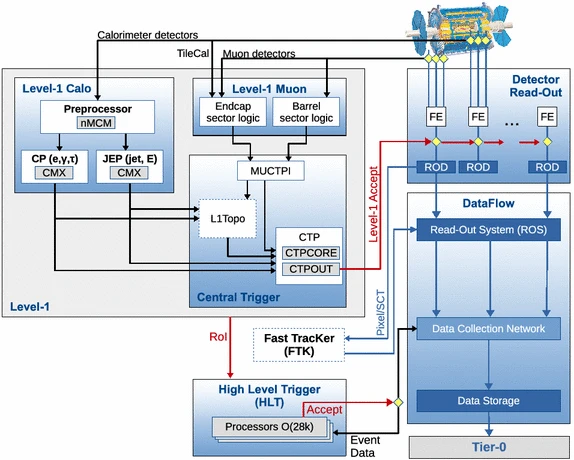
\includegraphics[width=\linewidth,height=\textheight,keepaspectratio]{trigger/trigger_flow}
        \caption{Flow chart of information through the ATLAS trigger system\cite{trigger_run2}.}
        \label{fig:trigger_flow}
    \end{figure}
    
    Triggering is achieved by running events through two sequential algorithmic systems.
    All events first go through the hardware-based Level 1 Trigger (L1) before being run through the more sophisticated (and slower) software-based High Level Trigger (HLT).
    Both of these systems involve a plethora of different measurements on various aspects of the events, such as total transverse energy, transverse momentum, jet multiplicity, and opening angles between jets.
    All of these measurements are used, alone or in combination, to decide whether or not an event passes the trigger selection.

    Each of the various kinematic properties checked by the triggers have multiple threshold values that can determine a ``pass.''
    For example, a jet $p_T$ trigger can have thresholds at 30, 45, or 55 GeV, among others.
    A ``trigger chain'' is a combination of several different such kinematic conditions, each with their own thresholds.
    A bunch crossing is ultimately accepted and read out to disk for further analysis offline if it is able to pass all the conditions of a trigger chain.
    There are hundreds of different trigger chains, each permitting different combinations of kinematics.
    An event is read out if it passes any one of these trigger chains, and is labeled in data with all the trigger chains it passes.
    The trigger chains used in ATLAS were largely decided upon before the beginning of the Run 2 data taking period\footnote{
        Some trigger chains were introduced later, as the trigger menu can evolve mid-run
        }, based on input from various analysis teams.
    This defined list of trigger chains comprise what is known as the ``trigger menu,'' and ultimately determines what kinds of physics processes ATLAS analyses have available.
    The following sections describe broadly how the two levels of the trigger system work, and later chapters will focus on which trigger menu items are used in the di-Higgs analysis specifically .

    \begin{figure}[h]
        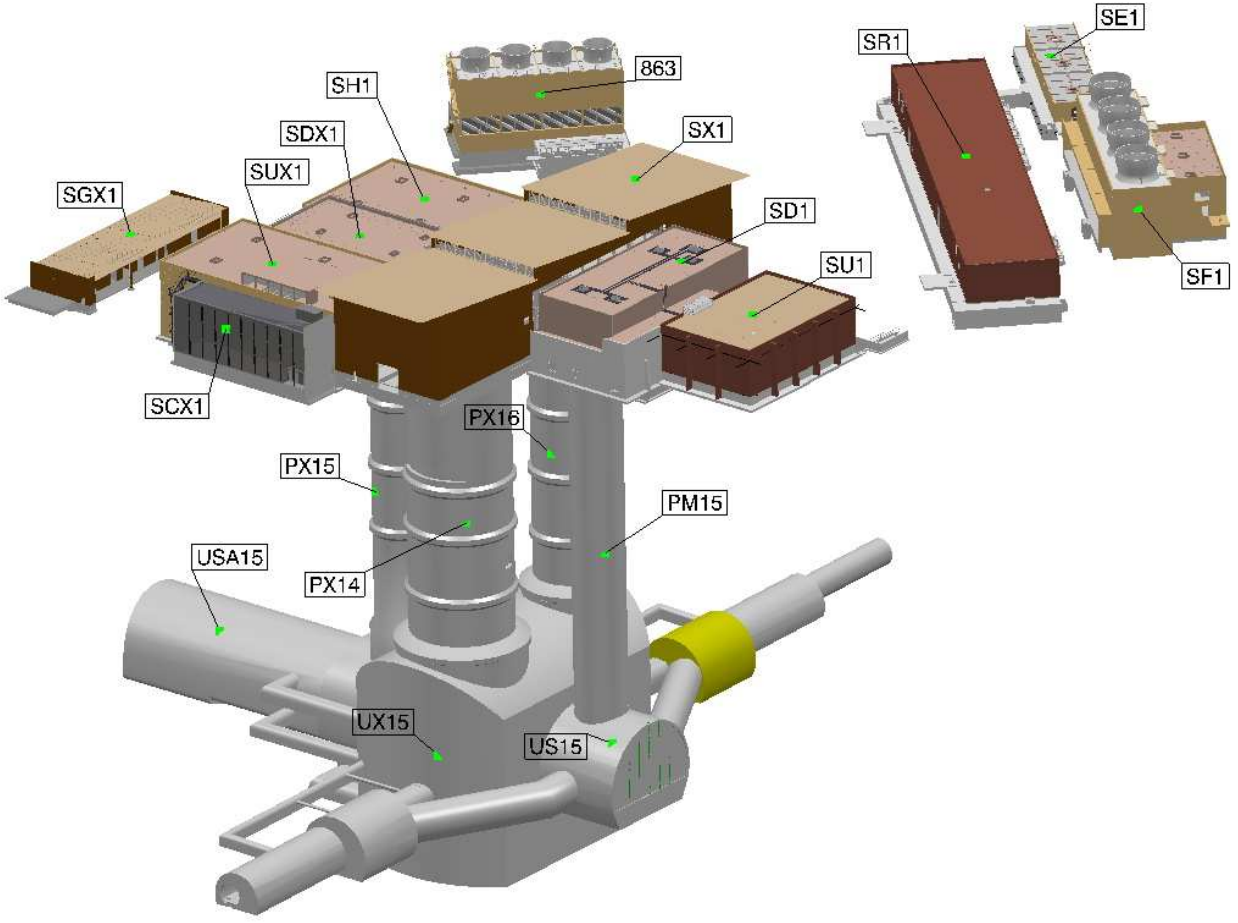
\includegraphics[width=\linewidth,height=\textheight,keepaspectratio]{trigger/facilities}
        \caption{General layout of buildings and facilities at LHC Point 1, site of ATLAS \cite{trigger_tdr}}
        \label{fig:facilities}
    \end{figure}


    \subsection{Level 1 Trigger}\label{sec:L1}

        One bunch-crossing every 25 ns is a blistering operational pace.
        The first layer of the trigger system, L1, therefore must run entirely through hardware-level gate logic.
        The goal of this system is to reduce the event rate from the raw 40 MHz bunch-crossing rate,
            down to a more computationally manageable rate of 100 kHz \cite{trigger_run2}.
        To reduce latency as much as possible, all the electronics comprising L1 are located as close as possible to ATLAS itself, specifically in the USA15 underground chamber \cite{trigger_tdr} (see Fig. \ref{fig:facilities}).
        An additional consequence of the high L1 operating frequency
            is that it must exclusively use information from the ATLAS calorimeters and Muon Trigger Chamber for its decisions.
        %(utilizes detector buffer memory to keep up).

        The Muon Trigger aspect of L1 is based entirely on the dedicated Muon Trigger Chambers, described in section \ref{sec:muon-trigger_chamber}.
        Their purpose is to make trigger decisions primarily based on muon $p_T$ and track multiplicity\cite{trigger_run1}.
        In the calorimeter-based trigger, the selection algorithm first requires a reduction in data resolution.
        The full granularity of the ATLAS calorimeters is too high to analyze in the 25 ns L1 has to process each bunch-crossing
            [TODO figure out Steve's edit to this :-/].
        Instead, the various sensors of the calorimeters are clustered together into ``trigger towers,''
            each with a resolution of $0.1 \times 0.1$ in $\Delta \eta \times \Delta \phi$.
        The way towers are clustered and used varies between the three different L1 calorimeter trigger modules.

        \begin{figure}[h]
            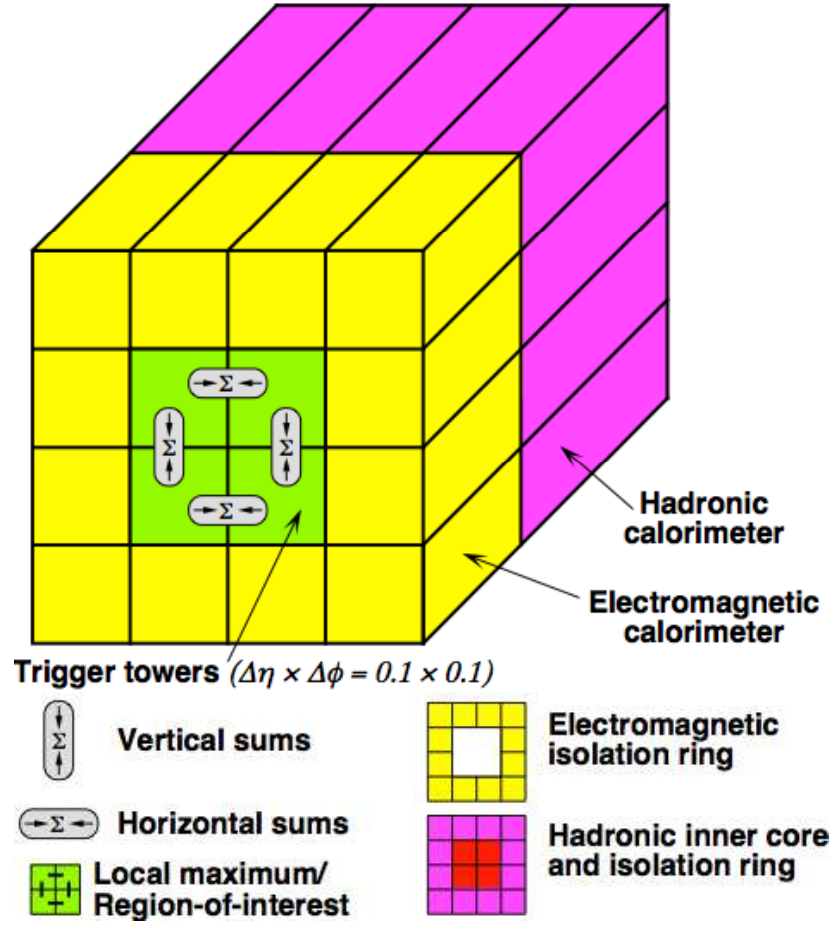
\includegraphics[width=\linewidth,height=\textheight,keepaspectratio]{trigger/trigger_towers}
            \caption{Structure of trigger towers and Regions of Interest \cite{L1_calo_run1}}
            \label{fig:trigger_towers}
        \end{figure}


        The Cluster Processor Module (CPM) exclusively uses the Barrel Calorimeters to function
            and is primarily meant for rapid identification of electrons/photons and taus/hadrons.
        For either case, the CPM's first step is to check all possible $4 \times 4$ ``windows'' of trigger towers, identifying windows containing an isolated ``Region of Interest'' (RoI).
        Here, an RoI is defined as a $2 \times 2$ cluster of towers with an $E_T$ sum that is a relative maximum compared to surrounding towers.
        This $2 \times 2$ RoI is the center of the $4 \times 4$ window (see Fig. \ref{fig:trigger_towers}).
        Windows are considered as passing the CPM trigger if the RoI satisfies an isolation requirement, meaning that the 12 towers surrounding that core fall \textit{below} a predefined $E_T$ ``isolation threshold'' value.
        Electrons and photons are then separated from taus and hadrons by the fact that the latter group penetrates into the HCal barrel, while the former group stays highly contained to the ECal.

        Expanding out, the Jet/Energy Processing Module (JEM, or sometimes JEP) makes use of the calorimeter barrels and endcaps, as well as the FCAL, though it does not distinguish between the ECal and HCal.
        The JEM further reduces the granularity under consideration, with a basic unit of data collection being $2 \times 2$ collections of trigger towers called ``jet elements,'' resulting in a minimum resolution of $0.2 \times 0.2$ in $\Delta \eta \times \Delta \phi$.
        Like the CPM, the JEM runs its trigger conditions on windows of multiple jet elements that must be based around a $2 \times 2$ RoI core (which is a local $E_T$ maximum).
        Unlike the CPM, these windows can vary in size.
        Primarily, the JEM is intended to perform hit multiplicity counting
            as well as assist the Extended Cluster Merger Modules (CMX) in carrying out the final jet multiplicity
            and $E_T$ sums \cite{L1_calo_run1}\cite{trigger_run2}.
        When these conditions, alongside those performed in the Muon trigger, are completed, the event is passed along to the HLT.


\FloatBarrier
    \subsection{High Level Trigger}

        After the L1 Trigger has reduced the event rate to 100 kHz, the software-based High Level Trigger is used to further reduce the event rate to the final output of \textasciitilde 1 kHz.
        Located in the SCX1 building (Fig. \ref{fig:facilities}) at the surface of P1 (again to minimize latency), the HLT uses data from all detector elements to completely reconstruct the event as it occurred in ATLAS, and performs its selections based on this reconstructed event.
        Different physics processes and particles, known as physics ``signatures,'' are reconstructed in different ways, and have different triggers based around them. 
        The main signatures used in ATLAS are: minimum bias signatures, electron/photons (Egamma), muons, jets, taus, missing transverse energy (MET), b-jets (as in jets from bottom quarks), and B-physics (as in B-hadrons).
        The process of reconstruction and the trigger algorithms applied to these reconstructed signatures are based on offline software algorithms which have been repurposed for online use.
        These offline algorithms are quite technical in nature, and are discussed further in Chapter \ref{chapter:reconstruction}.
        Once events have successfully passed both L1 and the HLT, they are finally distributed off-site for analysis by different physics groups.

        \begin{figure}[h]
            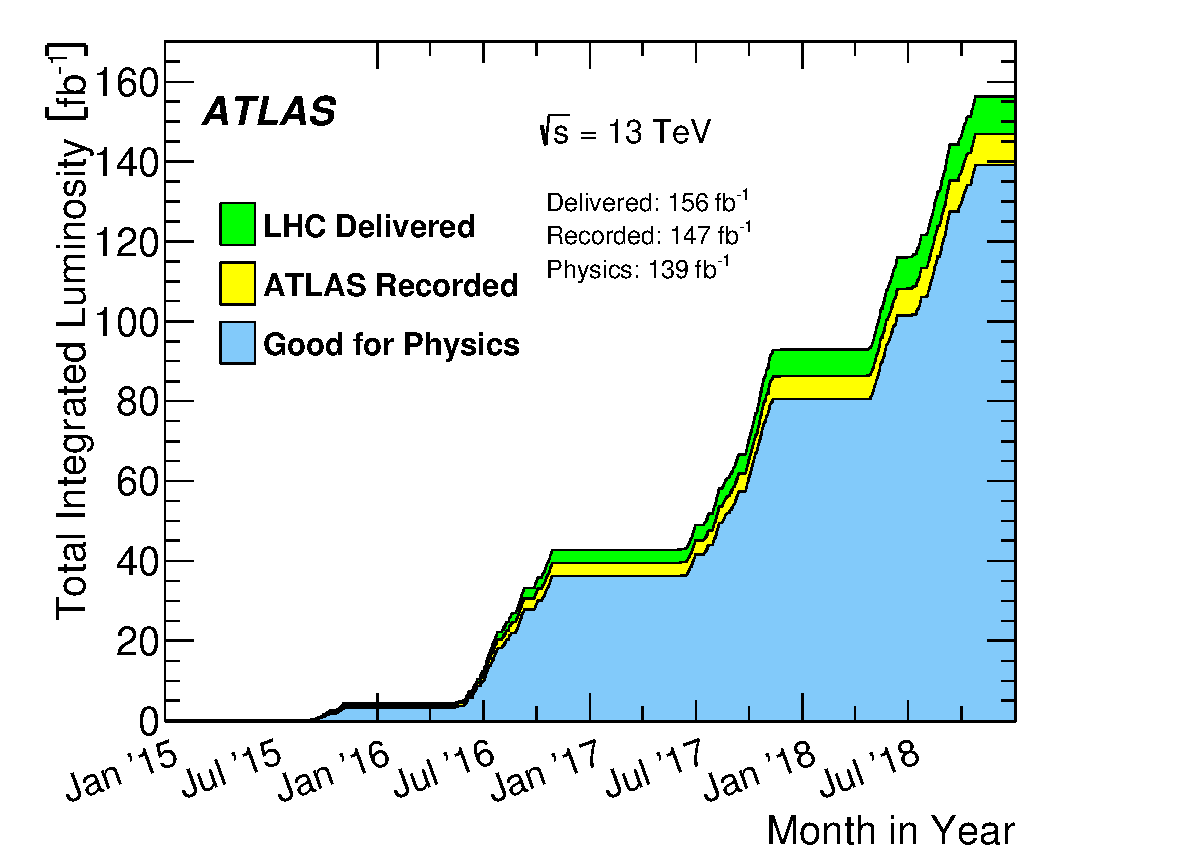
\includegraphics[width=\linewidth,height=\textheight,keepaspectratio]{trigger/data_delivered}
            \caption{Amount of data collected, in terms of integrated luminosity,
                through the Run2 data taking period\cite{data_quality}.
                ``LHC Delivered'' refers to the amount of luminosity present during stable beams.
                ``ATLAS Recorded'' is luminosity that the ATLAS decector was active and recording for.
                ``Good for Physics'' describes all the luminosity that was actually able to be passed to offline storage,
                    as opposed to thrown out because of malfunctions or issues in ATLAS at the time.
            }
            \label{fig:data_delivered}
        \end{figure}

        Over its three operational years, Run 2 has resulted in a total of 139 \ifb of data which has passed the online triggers
            (see Fig. \ref{fig:data_delivered}).
        Due to an inefficiency in the vertex reconstruction present during 2016,
            only 125.9 \ifb of that data are actually used in my analysis.
        Of that data, only a tiny portion is expected to be the actual di-Higgs signal event,
            which means further selection criteria will need to be applied.
        Understanding how the signal contribution is determined, and how these selections are optimized,
            requires understanding the second kind of data used for this analysis, Monte Carlo simulation data.




% Ch6: Reconstruction - DRAFT 2
\chapter{Event Reconstruction}

%    Once a bunch crossing event has cleared the Level 1 Trigger system, the process of event reconstruction begins.
%    An event in ATLAS is, initially, nothing but a collection of electrical signals emitted from the various detectors.
%    Event reconstruction is the process wherein detector readings are aggregated together into meaningful patterns,
%        which are interpreted as physical objects and processes.
%


    \section{Introduction}
        Ok let's just get the basic objects contructed first, since nothing else (triggers, later reconstruction, final selection)
            make sense until I have them.

        This entails ... what? For VBF 4b I think we have:


    %    I should have an image for this in some way %TODO
    \section{Tracks}
            
            %Intro about tracks being the first things we see because they're assembled from the inner detector or something.
            %Also I should probably explain what a track is...
        \subsection{Track Definition}
            
            The first point of contact for anything leaving the interaction region of ATLAS is the tracking detectors.
            Consequently, the objects reconstructed from the tracking detectors will be the first point of discussion.
            Prior to encountering the ATLAS calorimeters, particles exiting the IR travel along a relatively unimpeded trajectory.
            Thanks to the inclusion of the Solenoid Magnet field encompassing the Inner Detectors,
                these trajectories reveal crucial information about the particles in an event.
            This is due to the fact that any charged particle, with a momentum component orthogonal to a magnetic field,
                will trace out a \textit{helical} trajectory.
            If the shape of the helix is known, then basic electrodynamics principles can be used to determine the
                momentum, charge, and mass of the particle that formed it.

            To see how this can be done, 

            



            Might need to explain helix parameters as well
            \cite{thesis_track_sim_and_reco}
            \cite{charged_particle_tracking}

        \subsection{Track Reconstruction}

            As particles pass through the inner detector subsystems, they trace out a path of ionized detector elements.
            The trajectory can be reconstructed by playing connect the dots.

            %Clusterization
            The first step to producing a track is the process of clusterization.
            Ionizing particles often deposit energy across several adjacent pixels on a given layer.
            A \textit{connected component analysis} algorithm is used to group pixels together. 
            Based on the pattern of energy distribution in these groups,
                a \textit{space-point} is created indicating the estimated position at which a particle crossed the detector.
            Several space-points can be assigned to the same pixel cluster,
                if the energy deposition pattern suggests multiple particles traversed the same location.

            %Combinatorial track finding
            Initial guesses at tracks, called track seeds, are formed by assembling all realistic combinations of three space-points.
            The track seeds are assigned helix parameters by assuming they travel through a uniform magnetic field,
                allowing immediate estimates of the tracks' momentum.
            These seeds are expanded into \textit{track candidates},
                by including more space-points across additional detectors in the ID using a \textit{Kalman filter}.

            %Ambiguity solving; NN clustering; Track fit
            A number of criteria are then used to reject poor-quality tracks, as well as to assign scores to all remaining track candidates.
            The scores are then used to resolve ambiguities where multiple tracks are assigned to the same space-points,
                with preference given to higher-scoring candidates.
            Neural networks are used to assist in some ambiguity solving situations,
                as well as to help identify clusters with multiple valid tracks.
            Once ambiguities have been resolved and all malformed track candidates removed,
                the remaining tracks are refit using all available information at high-resolution.
            \cite{atlas_track_reco_performance}

    \section{Jets}
        Jets are an algorithm.
        Specifically, the anti-$k_t$ algorithm, with $\Delta R = 0.4$.
        Something about topological-clusters (topo-clusters).
        \cite{anti_kt}
        Something about assuming hard-scatter jets come from the primary vertex.
        Also explain what a primary vertex is.
        FYI, a primary vertex is a "reconstructed vertex with at least two associated tracks, and the largest sum of squared track momentum".

        Jets created using only calorimeter-based topological-clusters (at the electromagnetic scale [what does this mean??]) %TODO?
            are reffered to as \textit{EMtopo Jets}.
        The jets for this analysis use a more advanced jet algorithm, called \textit{Particle Flow},
            which are constructed by matching tracks from the inner detector to topo-clusters from the calorimeter,
            based on both location and energy projections.
        The resulting \textit{PFlow Jets} are then used for the rest of the reconstruction process.
        \cite{pflow}
        \cite{jet_energy_scale13TeV}

    \section{Flavour Tagging}
        Of crucial importance:
            b-jets used for higgs,
                (I should justify this with the high branching ratio of H->b,bbar;
                you put this in your thesis commitee talk, use it);
            VBF initial scatter jets anti-b-tagged

        Flavour Tagging is performed in two-stages:
            first with basic low-level taggers,
            which are then used as inputs for the high level taggers.

        \subsection{Low Level Taggers}

            IPxD - IP2D and IP3D - Impact Parameter 2/3 Dimensional; 

            Vertex Algos - SV1 (Secondary Vertex 1) and JetFitter
            \cite{thesis_giacinto}

        \subsection{High Level Taggers}

            MV2, a Boosted Decision Tree (BDT);
            DL1, a Deep Learning Neural Network (DL1r is what we specifically use)
            \cite{bjet_id_and_performance}
            \cite{btagging_optimisation}

    \section{Online VS Offline Reconstruction}
        I should explain how online and offline reco differs;
            it seems to just come down to the fact that the HLT doesn't neccesarily use the most high resolution calorimeter information,
            and often generates tracks using a faster, less acurate algorithm.

        Reconstruction is performed for an event twice.
        It is first done rapidly, using coarse measurments and calculations,
            for the purpose of allowing the aforementioned HLT to trigger events for readout.
        These events which pass the trigger are passed off to a massive global computer cluster reffered to as the GRID.
        No longer bound by the stringent time contrainsts of the ``online'' running environment,
            the GRID is able to devote vast amounts of time and computing power to a second, 
            more comprehensive, reconstruction of each event.
        For both the ``online'' (HLT) and ``offline'' (GRID) environments, event reconstruction is carried out by the same suite of software,
            called \textit{Athena}.
            
        I should also describe the mv2 reweighting procedure here
            (We don't use mv2 for the late-stage b-tag requirement on the higgs decay candidates,
            but we DO use it in the triggers):
            Step1.1 - Run HLT reco on MC files;
            Step1.2 - Return low level taggers on MC HLT reco;
            Step2   - Rerun HLT reco on MC, now with retuned low level tagging info;
            Step3.1 - Perform BDT training for MV2 on HLT MC reco w/ low level tags;
            Step3.2 - Convert training output to useable histograms;
            Step4   - Rerun HLT reco on MC once more, to get full retuned tagging ouput. Use output performance to determine working points;


    \section{Scale Factors}
        
        Ugghhh... I wonder if this should go up into the trigger chapter? Might make more sense


% Ch7: Selection - DRAFT 2
\chapter{Event Selection} \label{chapter:selection}

\section{Introduction}

    In parallel with the process of reconstruction, is that of event selection.
    As was mentioned earlier in the discussion of the ATLAS Trigger,
        there are far too many events in ATLAS to analyze them all.
    Thus, a series of selection algorithms are used to veto the abundance of background events.
    Unfortunately, these selection algorithms are not perfect,
        and so a careful balance must be attained between removing a suitable amount of background,
        while retaining as many signal events as possible.

    \begin{figure}[tbh]
        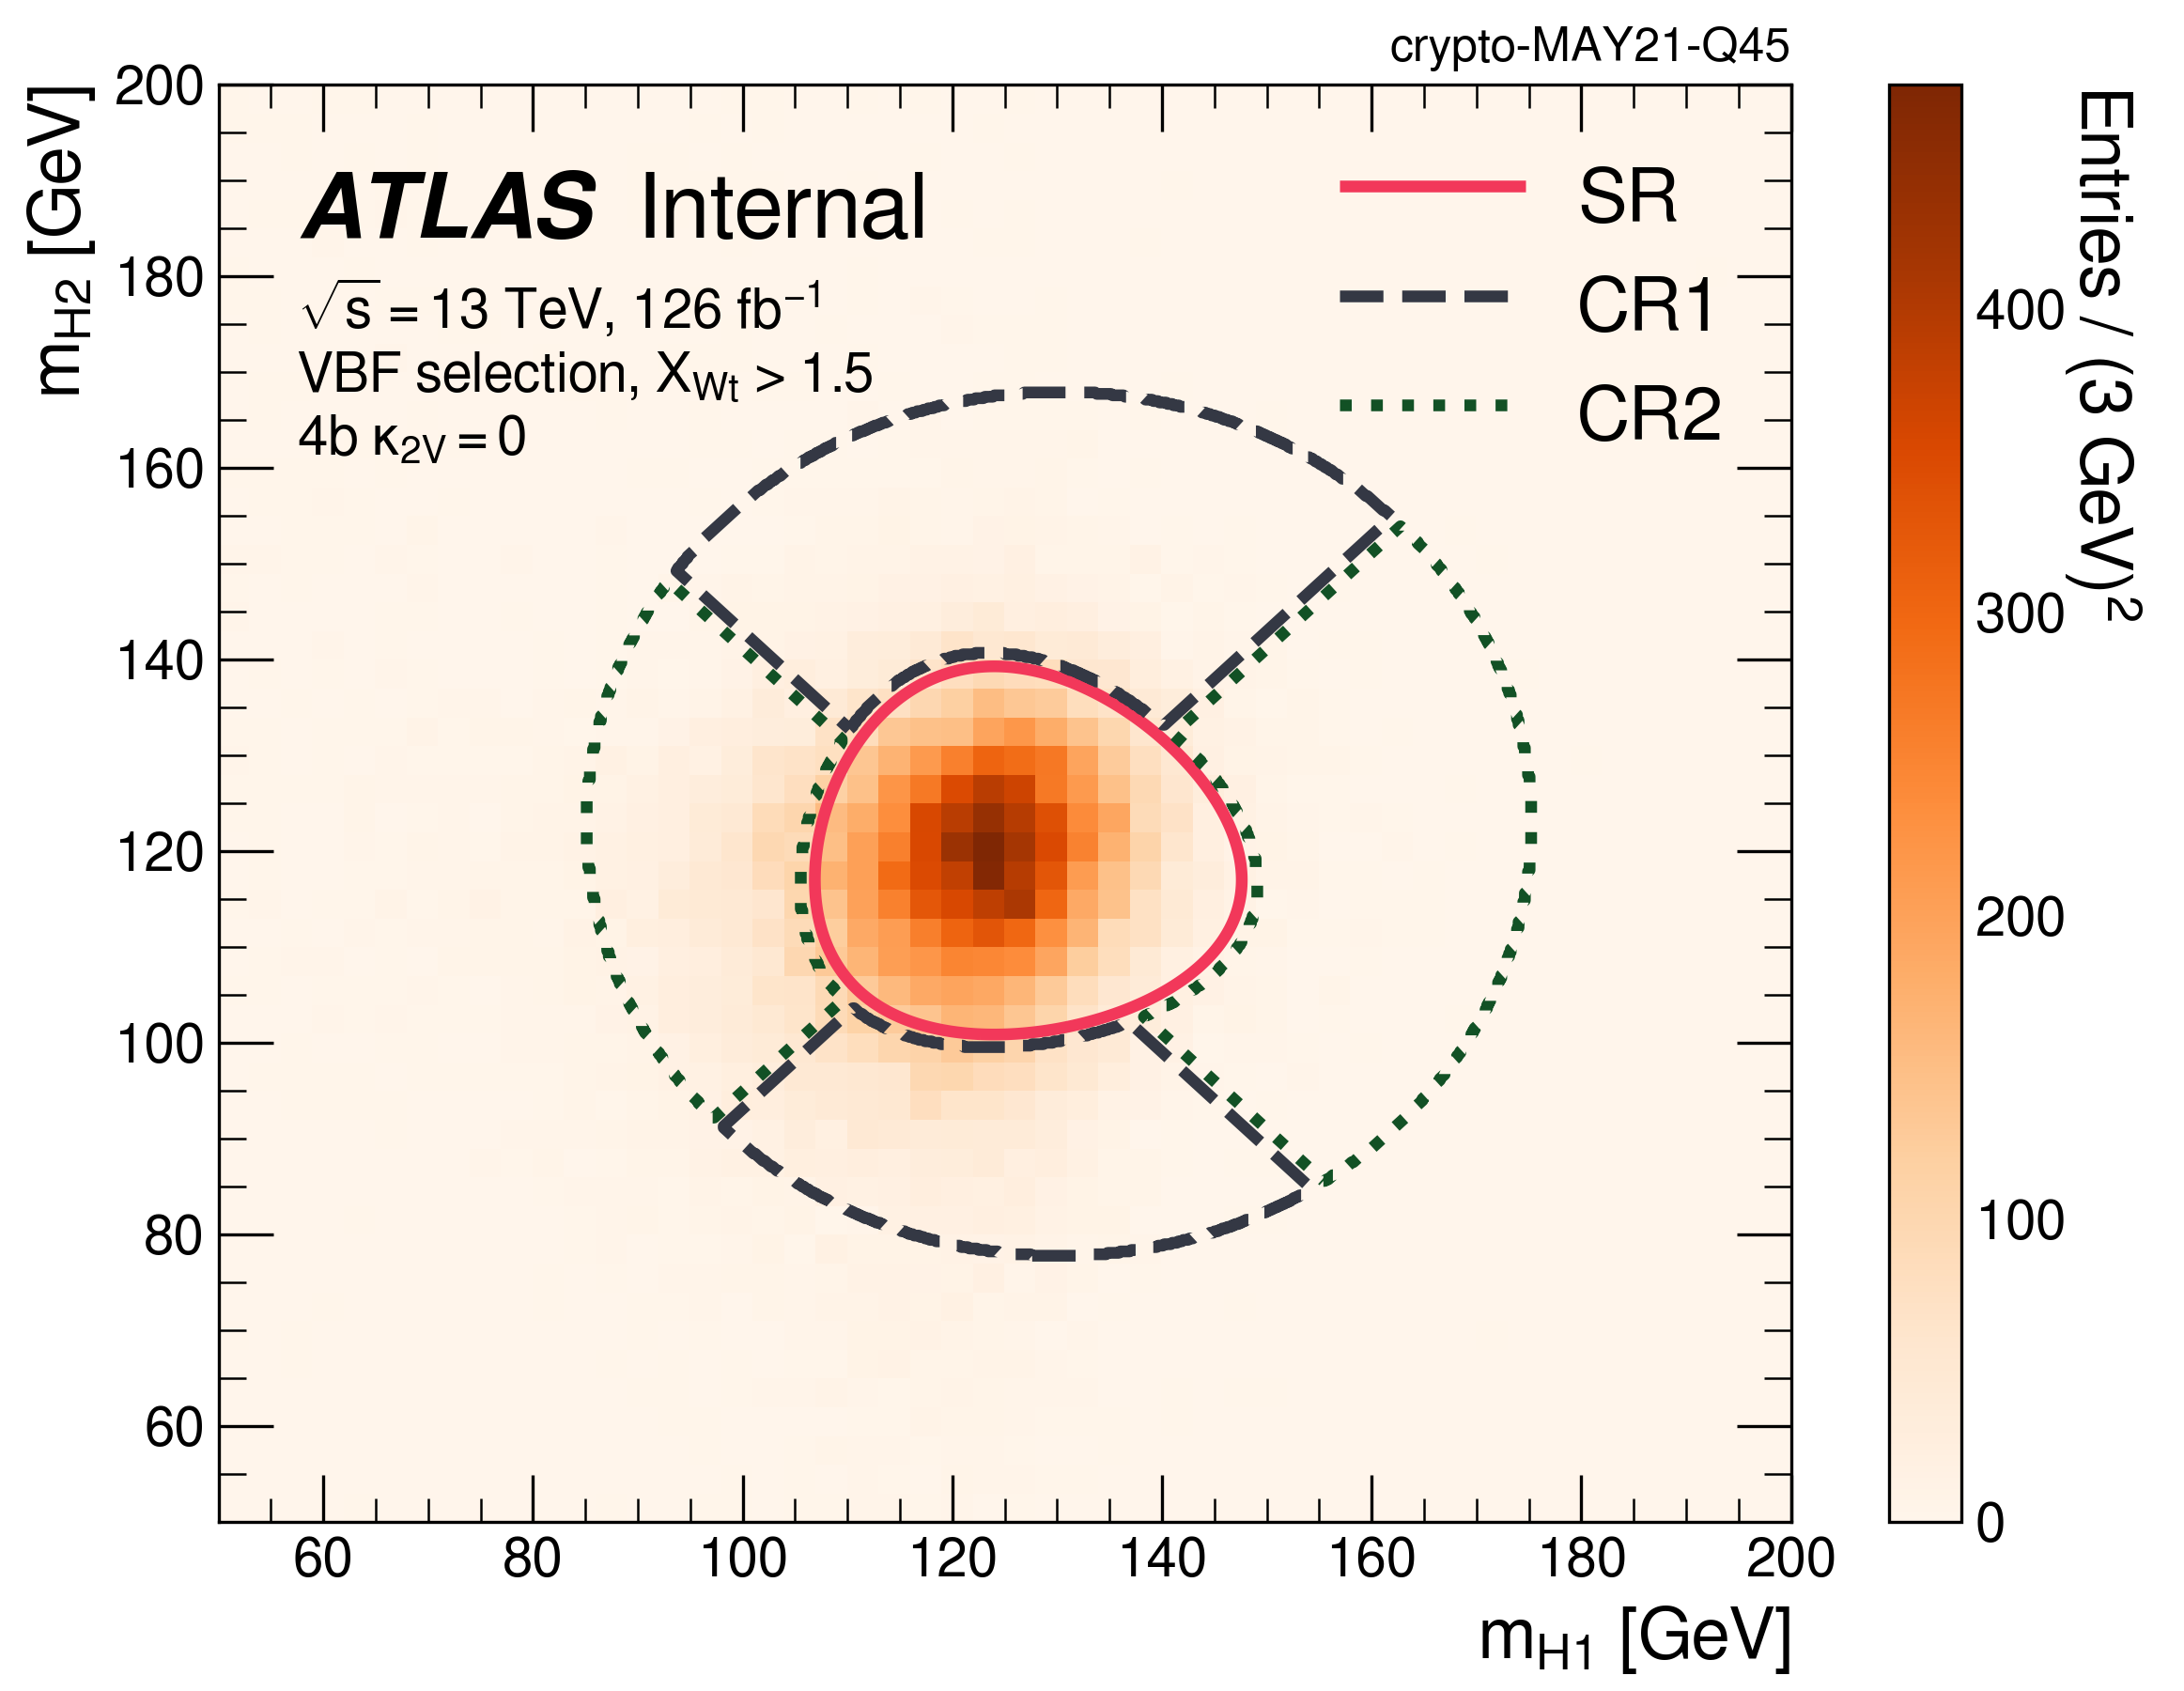
\includegraphics[width=\linewidth,height=\textheight,keepaspectratio]{selection/massplane_sig_all_4b_vbf_Xwt_1.5_k2V_0}
        \caption{
            TODO; FIXME
        }
        \label{fig:event_display}
    \end{figure}

    %TODO also don't forget all the truth-level validation plots you have just LAYING AROUND ALREADY
    % that you can dump in here as a demonstration of probably any point you want to make
    
    Figure \ref{fig:event_display} is an ``event display'' of what a VBF \to 4b event is expected to look like,
        based on Monte-Carlo simulation (see Chapter \ref{chapter:signal}).
    It demonstrates the key features these selection algorithms use to differentiate signal from background.
    The most obvious feature to identify is the high-$p_T$ jet multiplicity.
    VBF \to 4b will invariably produce a total of six jets;
        the two initial-scatter (IS) light-quark jets, plus the 4 b-jets from the Higgs decay.
    All six of these jets will carry significant energy and transverse momentum.
    A hallmark of the VBF process is the wide opening angle and high invariant mass between the IS jets.
    Such a jet pattern stands out dramatically from most of the stochastic background noise,
        one of the main advantages of the VBF process.
    Additionally, while the four b-jets of the Higgs are not exclusively produced in the low-$\eta$ regions,
        so many high-$p_T$ b-jets orthogonal to the beamline is extremely rare for background events,
        and thus makes for another highly identifiable feature of the signal.
    Something something bjet decays close together.




    The initial selection process is carried out before and during reconstruction, via the aforementioned trigger system.
    After the primary reconstruction process, an additional set of selection criteria,
        specific to this analysis,
        are applied to the fully reconstructed event objects.

    
    %I need to discuss the kinematics of VBF and 4b in order to justify the ->
    \FloatBarrier

    \section{Triggers}
        
        The first stage of the Selection process occurs, to some degree,
            before reconstruction has even begun, in the L1, HLT, and Offline ATLAS Triggers.
        Table \ref{tab:nr-triggers-used} lists the trigger chains used in this analysis.
        An event from ATLAS is incorporated into the data used in this analysis as long as it passes at least one 
            of the listed chains associated with its year.
        These triggers have been chosen based on any features that lend themselves to the VBF \to 4b process.
        Noteably, the triggers in use heavily emphasize high jet multiplicity and an abundance of b-jets
            (both integral to VBF \to 4b).
        To understand how, it is necessary to understand the nomenclature of the trigger chains.
        A full reference can be found in ??, but a brief example of how to read the chains is provided here:

        HLT\_j110\_gsc150\_boffperf\_split\_2j45\_gsc55\_bmv2c1070\_split\_L1J85\_3J30:
        \begin{itemize}
            \item HLT: Most of the following requirements are based in the High Level Trigger
            \item j110: Requires one 110 GeV jet
            \item gsc150: Cut on jet $p_T \geq 150$ GeV after Global Sequential Calibration (GSC) algorithm is applied
            \item boffperf: b-jet Offline Performance algorithm
            \item split: Using ``Split'' track reconstruction algorithm
            \item 2j45: Find 2 jets with $p_T$ of at least 45 GeV
            \item gsc55: Cut on jet $p_T \geq 55$ GeV after GSC algorithm is applied
            \item bmv2c1070: passes b-jet MV2c10 algorithm at 70\% efficiency level
            \item split: (as above)
            \item L1J85: Level 1 Trigger algorithm requiring a cluster with an energy of at least 85 GeV 
            \item 3J30: Require at least 3 jets with a minimum $p_T$ of 30 GeV
        \end{itemize}


        \begin{table}[htbp]
\centering \footnotesize
\begin{tabular}{ccc}
Year                      & Trigger Name                                                                    & \textbf{Trigger Type}  \\ 
\hline
\multirow{2}{*}{2016}                      & HLT\_j100\_2j55\_bmv2c2060\_split                                               & 2b1j                   \\
                      & HLT\_2j35\_bmv2c2060\_split\_2j35\_L14J15.0ETA25                                & 2b2j                   \\

\hline

\multirow{2}{*}{2017}                      & HLT\_j110\_gsc150\_boffperf\_split\_2j35\_gsc55\_bmv2c1070\_split\_L1J85\_3J30  & 2b1j                   \\
                      & HLT\_2j15\_gsc35\_bmv2c1040\_split\_2j15\_gsc35\_boffperf\_split\_L14J15.0ETA25 & 2b2j                   \\

\hline

\multirow{2}{*}{2018}                      & HLT\_j110\_gsc150\_boffperf\_split\_2j45\_gsc55\_bmv2c1070\_split\_L1J85\_3J30  & 2b1j                   \\
                      & HLT\_2j35\_bmv2c1060\_split\_2j35\_L14J15.0ETA25                                & 2b2j                   \\
                
\end{tabular}
\caption{Triggers used for non-resonant searches.\cite{hh4b_2021_int_note}}
\label{tab:nr-triggers-used}
\end{table}


        % Triggers used in this analysis and why
        % (do we have any plots showing why we use these triggers?)
        %   Yes, though I might be able to get away without using them

        %Trigger bucketing strategy? What are the chances I can just not deal with this?


    \section{Analysis Cuts} \label{sec:analysis_cuts}

        After the triggers, a number of other things are cut on.

    \subsection{Jet Multiplicity and Categorization}

        Central Jets are defined as those within $|\eta| \leq 2.5$
            (to ensure these jets have passed through the tracker, which is needed for the b-tagging tools\cite{vbf_hh_4b_resonant_2018_int}),
            with pt > 40 GeV and which pass JVT or have pt > 60 or have |eta| > 2.4. %I think these are just more trigger things
        
        Forward Jets are those with $ 2.5 < |\eta| \leq 4.5 $, 
            with pt >= 30 GeV %Pretty sure this is just a trigger threshold

        Must have at least six total central and forward jets.
        At least four of the jets must be b-tagged central jets.
        At least two of the jets (forward or central) must be anti-btagged.

        The Higgs decay jets are chosen as the four highest-pt, b-tagged, Central jets.
        The VBF jets are chosen as the pair of anti-btagged jets (central or forward)
            with the largest vector-sum invariant mass (mjj) between them.
        %TODO: I should probably provide a source that does this, since it's common practice
        % Maybe pull up one of the papers Ariel had you read?


    \subsection{VBF Topology}
        
        The selected VBF pair must have a \deta between them of at least 3,
            and an mjj of at least 1 TeV.
        As well, the combined vector-sum-pt of all six jets
            (the four Higgs products and the two VBF jets)
            must be less than 65 GeV.
        (See Figure \ref{fig:vbf_cuts})

        \begin{figure}[tbh]
            \subfloat[$m_{jj}$ Cut Significance]{
                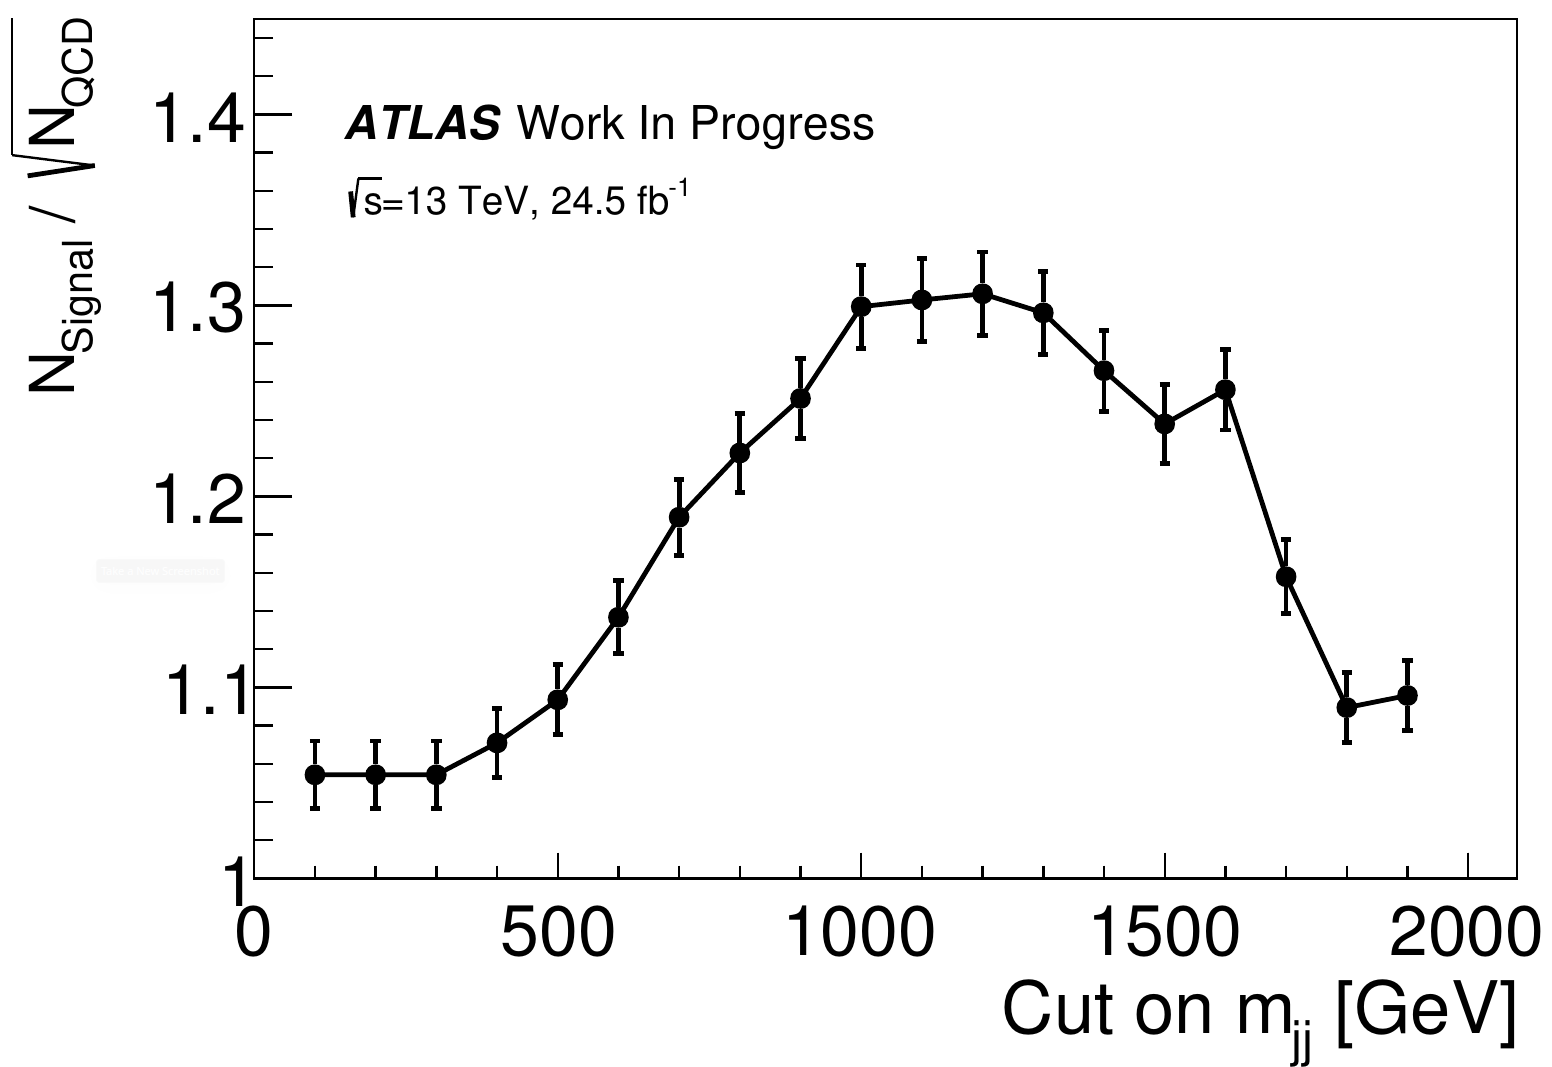
\includegraphics[width=0.5\linewidth,height=\textheight,keepaspectratio]{selection/mjj_significance}
            }
            \subfloat[$\deta_{jj}$ Cut Significance]{
                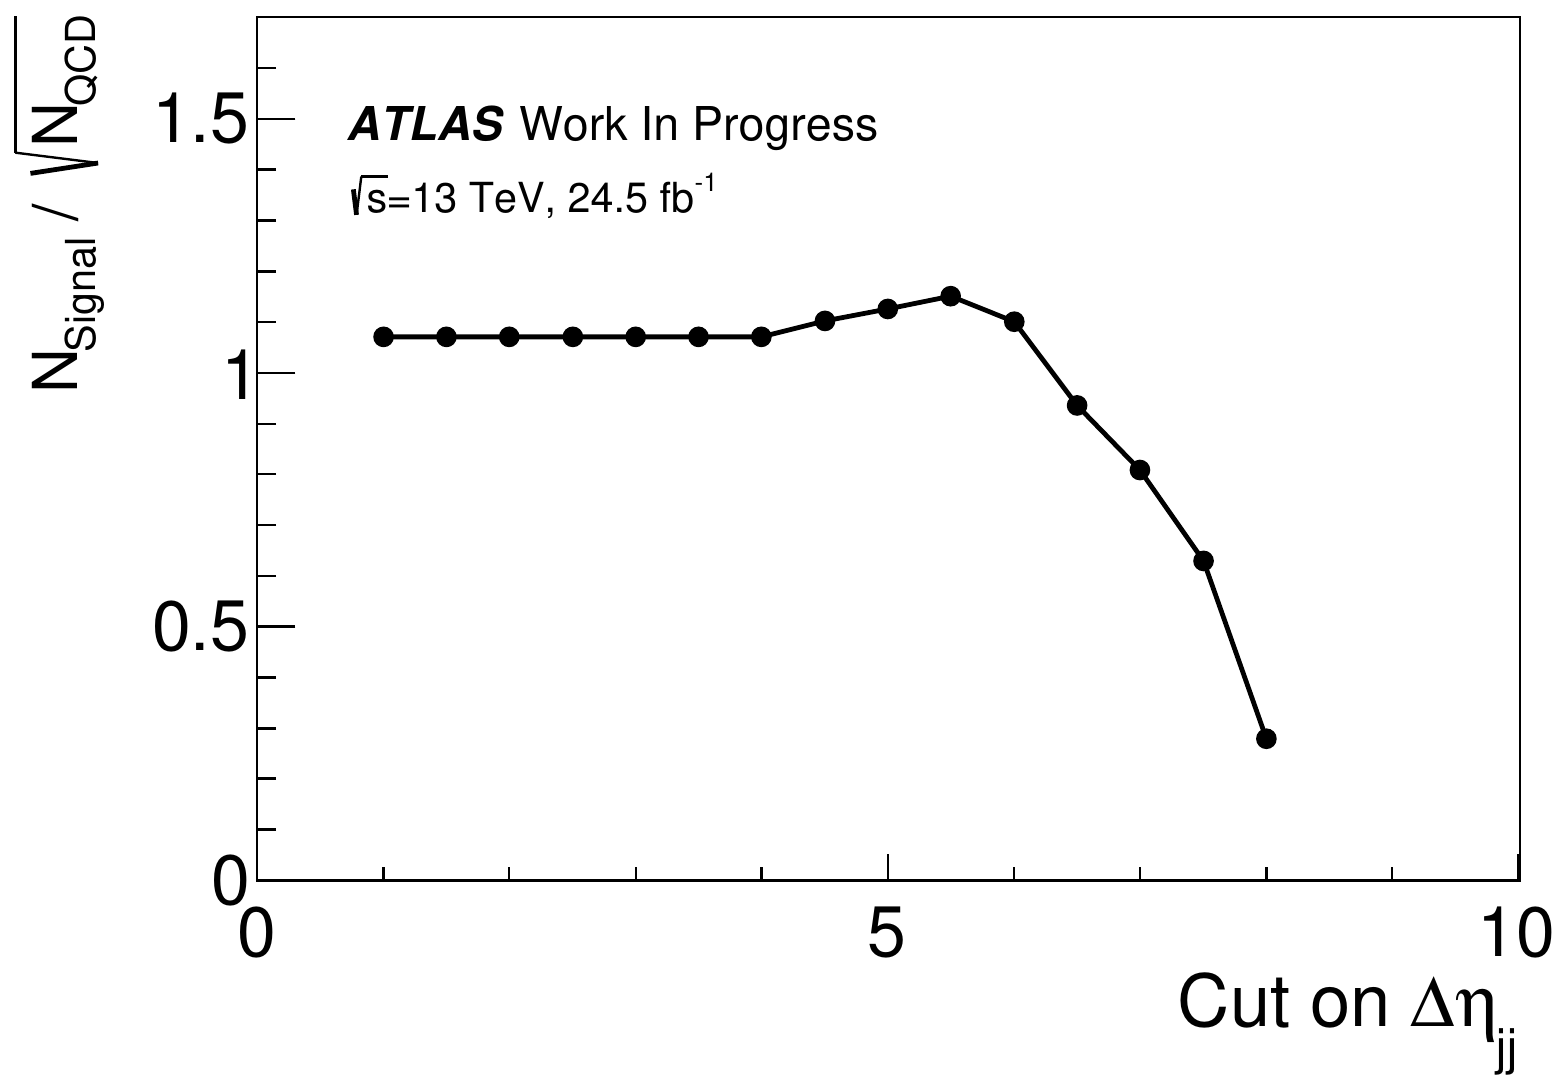
\includegraphics[width=0.5\linewidth,height=\textheight,keepaspectratio]{selection/detajj_significance}
            }\\
            \subfloat[6-Jet Vector-Sum $p_{T}$ Cut Significance]{
                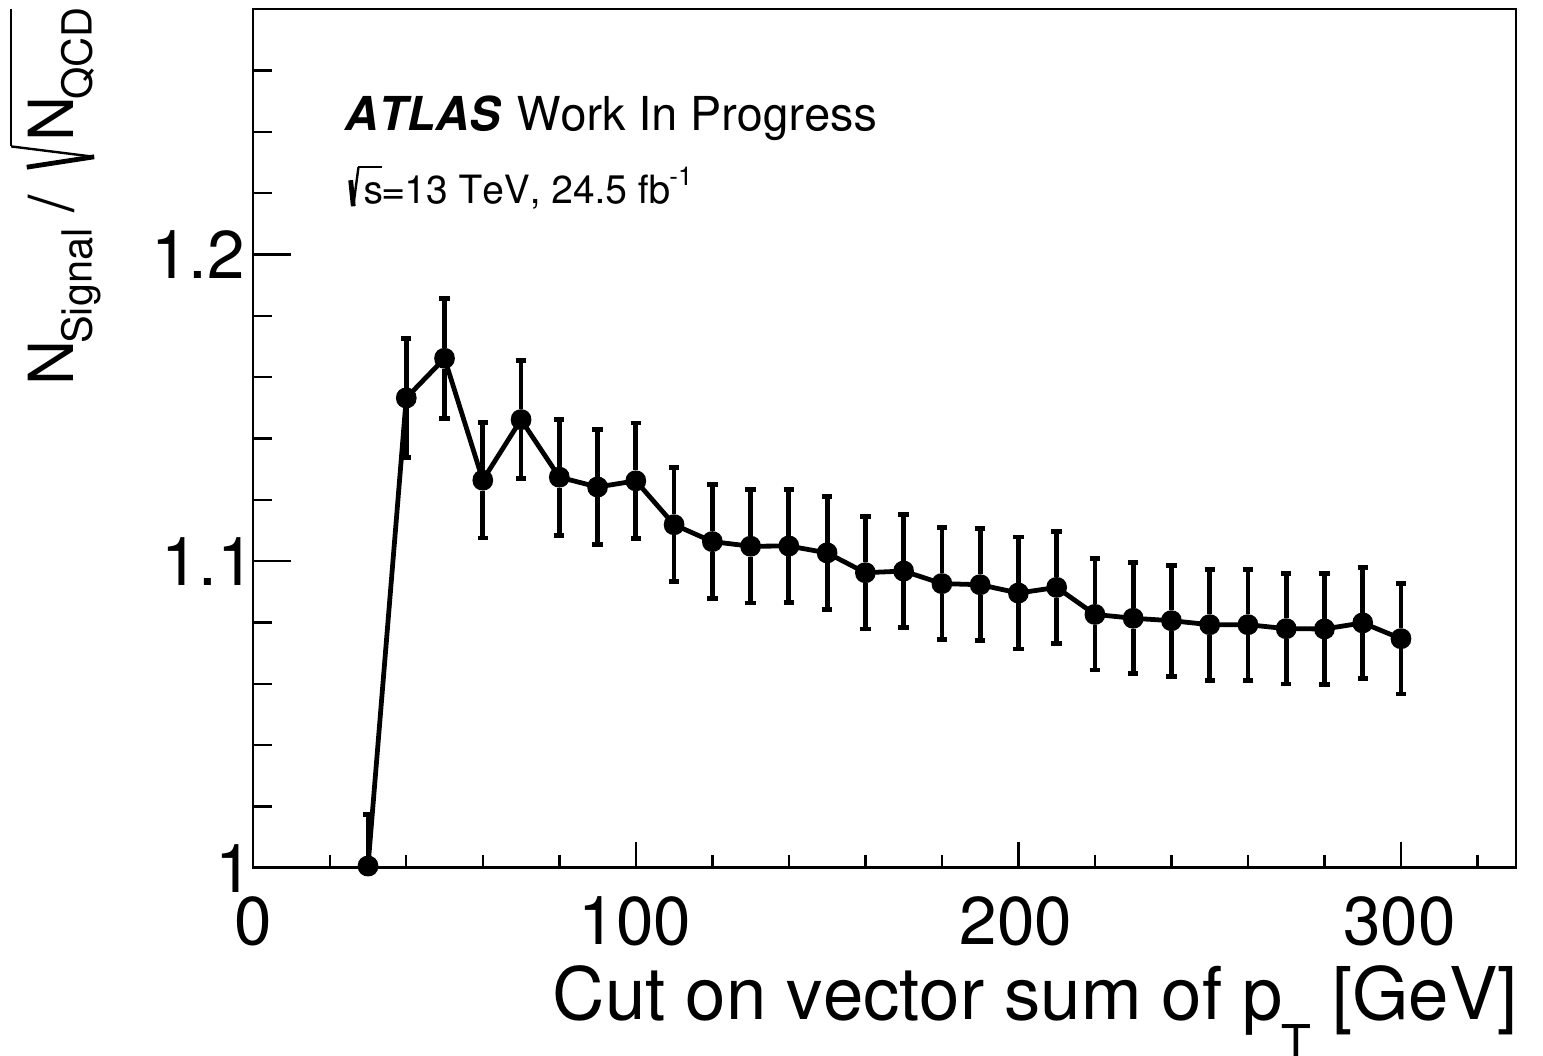
\includegraphics[width=0.5\linewidth,height=\textheight,keepaspectratio]{selection/vecsum_pt}
            }
            \caption{
                Significance value (see Chapter \ref{chapter:results})
                    for different cut values on the various VBF selection criteria\cite{vbf_hh_4b_2018_int}.
                TODO: I might need to replace these (especially the detajj one... that or our current cuts are super wrong).
            }
            \label{fig:vbf_cuts}
        \end{figure}
        \FloatBarrier


    \subsection{B-Quark Pairing}
        
        What is detected within ATLAS and reconstructed by Athena are not Higgs Bosons, but rather their decay products.
        To reconstruct the two Higgs Bosons, the four reconstructed b-quarks must be combined together, two b's to each Higgs.
        A pairing algorithm, called MinDR \cite{hh4b_2021_int_note},
            is used to determine which b-quarks should be paired to each other.
        MinDR operates under the assumption that the decay products of the Higgs boson
            should be relatively close to each other in angular space, maintaining the Higgs' high $p_T$.
        With four jets, which need to be split into two pairs, there are three ways to choose the pairings.
        For each of the three pairing options, MinDR takes the pair with the leading $p_T$ as the ``leading Higgs Candidate''
        The pairing option which is chosen is that which minimizes the $\Delta R$ between the leading Higgs Candidate decay products
            (see Figure \ref{fig:minDR_pairing_diagram}).
        The effectiveness of this algorithm has been validated for multiple values of \kvv and \kl,
            as shown in Figure \ref{fig:HHpairing}.

        \begin{figure}[tbh]
            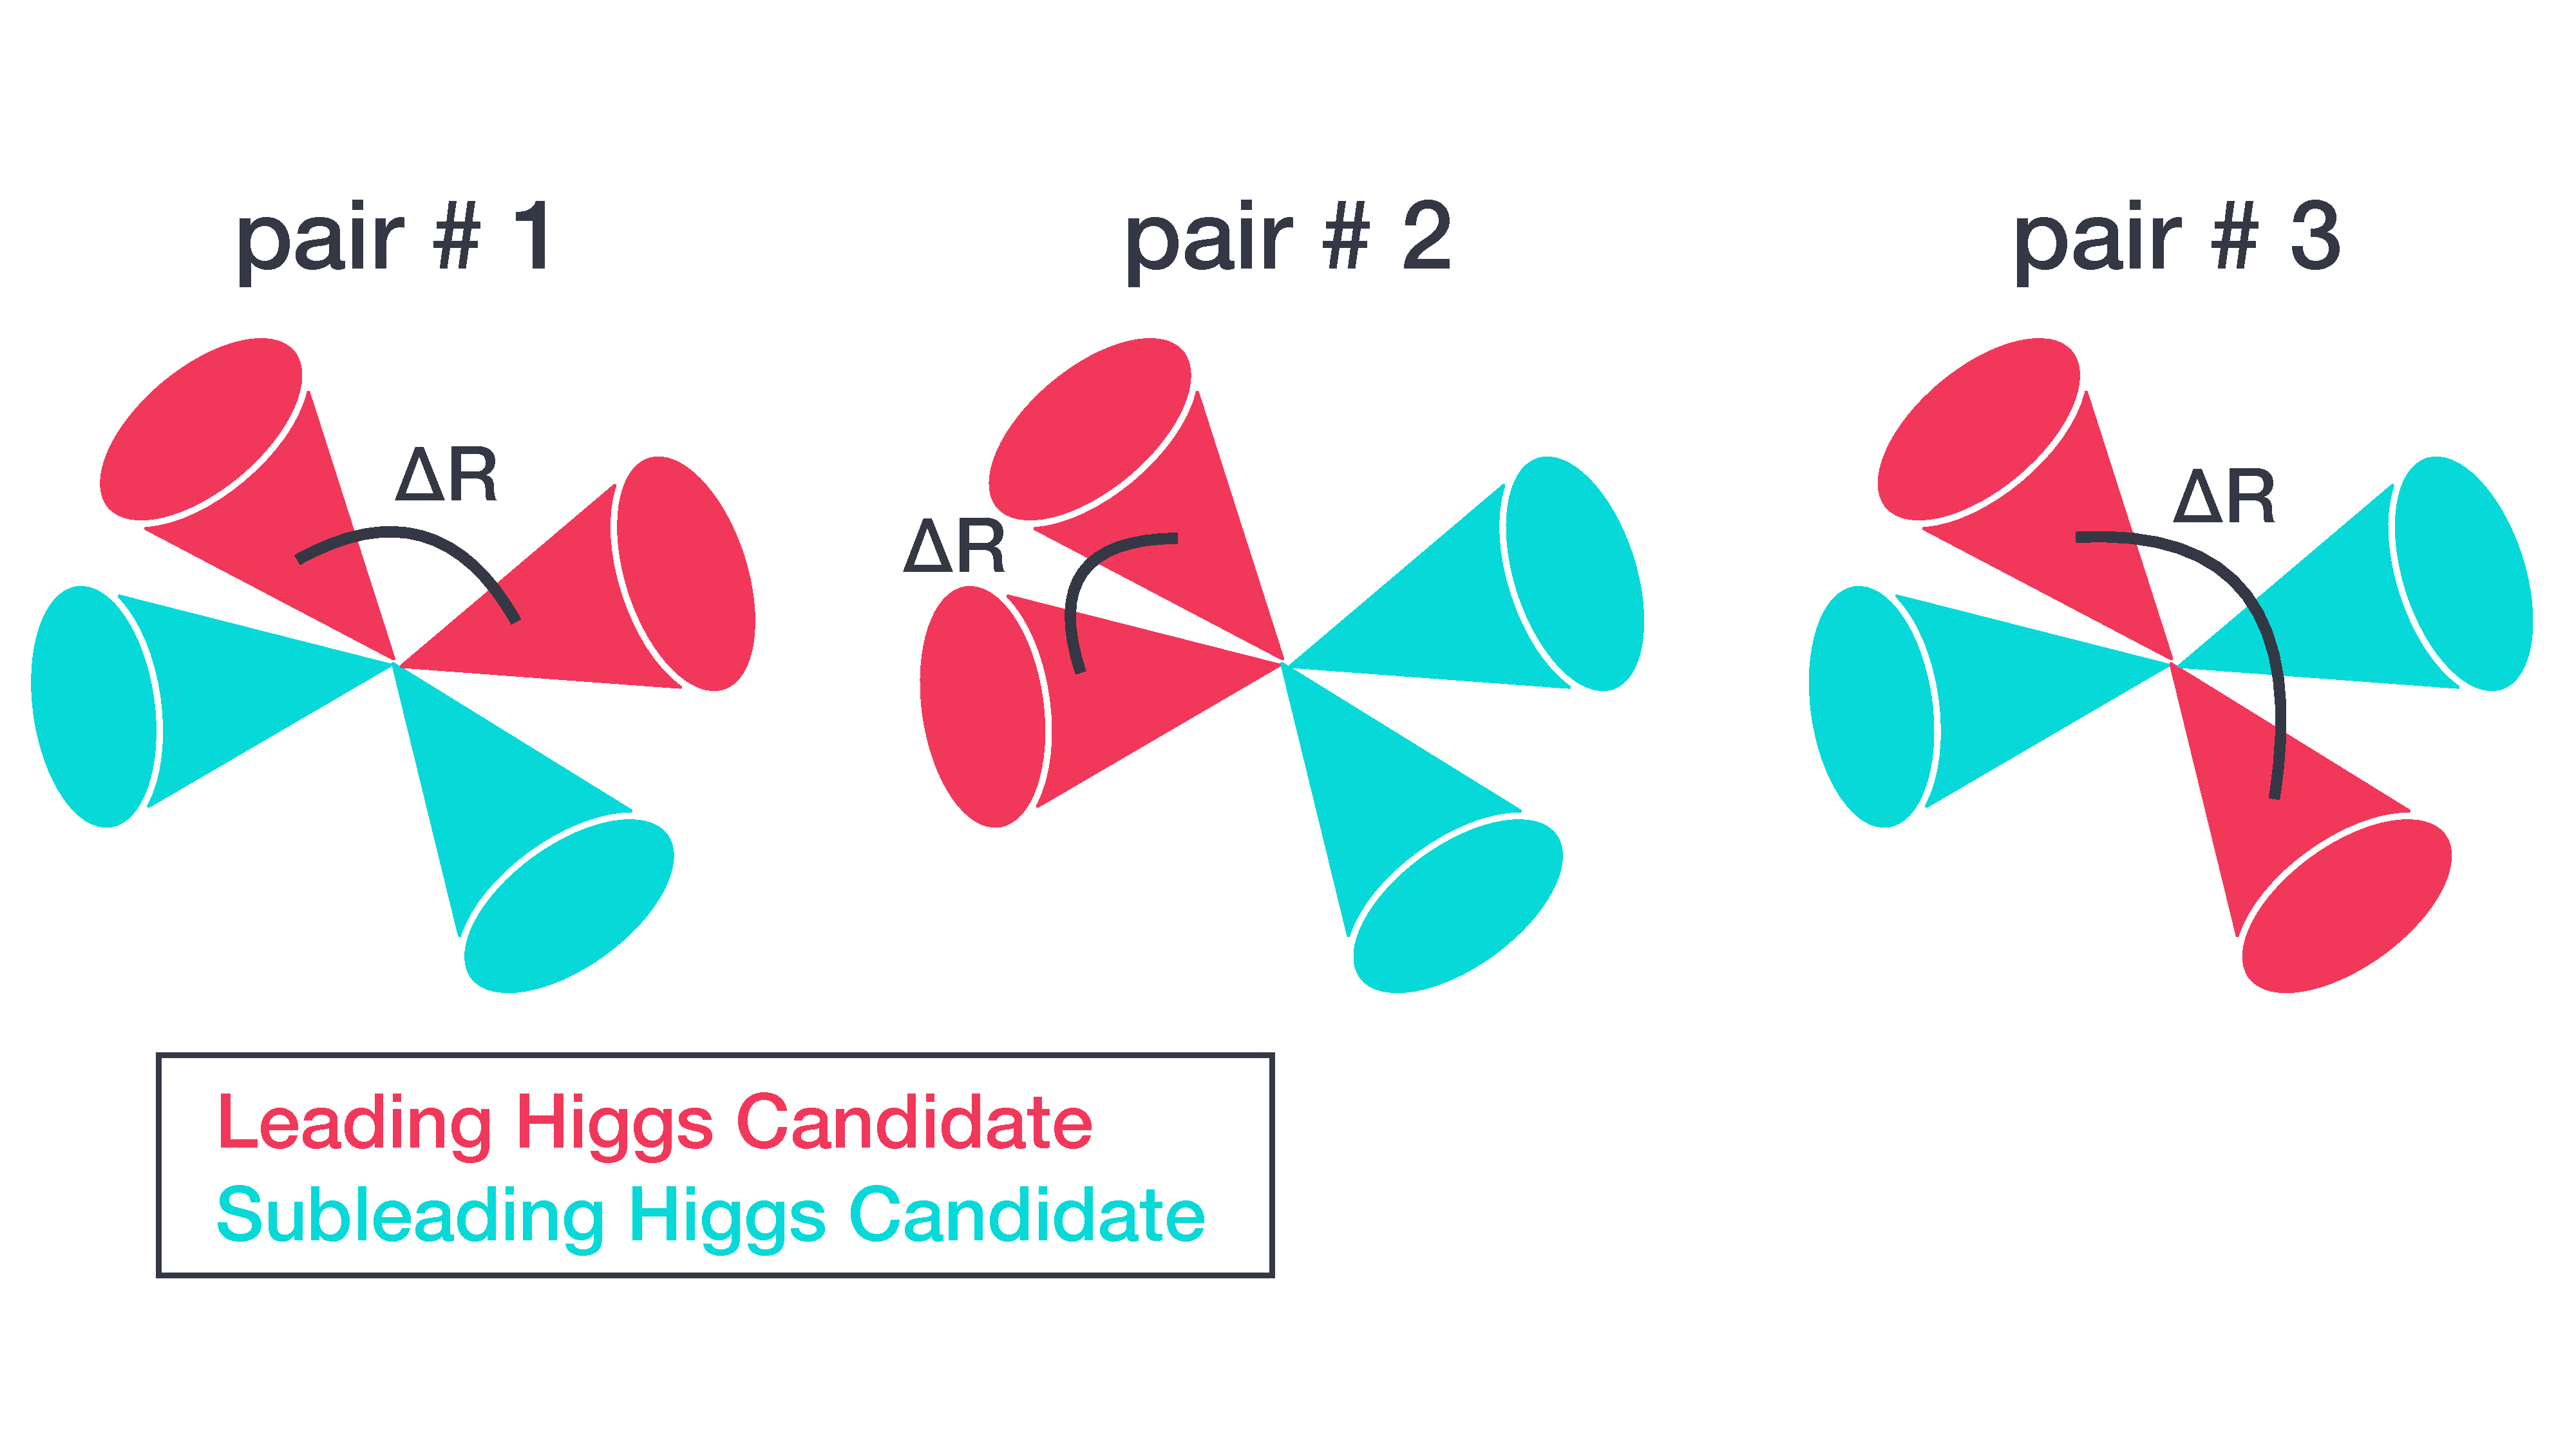
\includegraphics[width=\linewidth,height=\textheight,keepaspectratio]{selection/pairing}
            \caption{
                TODO (minDR picks pair 2 btw)\cite{hh4b_2021_int_note}
            }
            \label{fig:minDR_pairing_diagram}
        \end{figure}

        \begin{figure}[hbt]
            \centering
            \subfloat[Pairing accuracy vs \kl]{
                     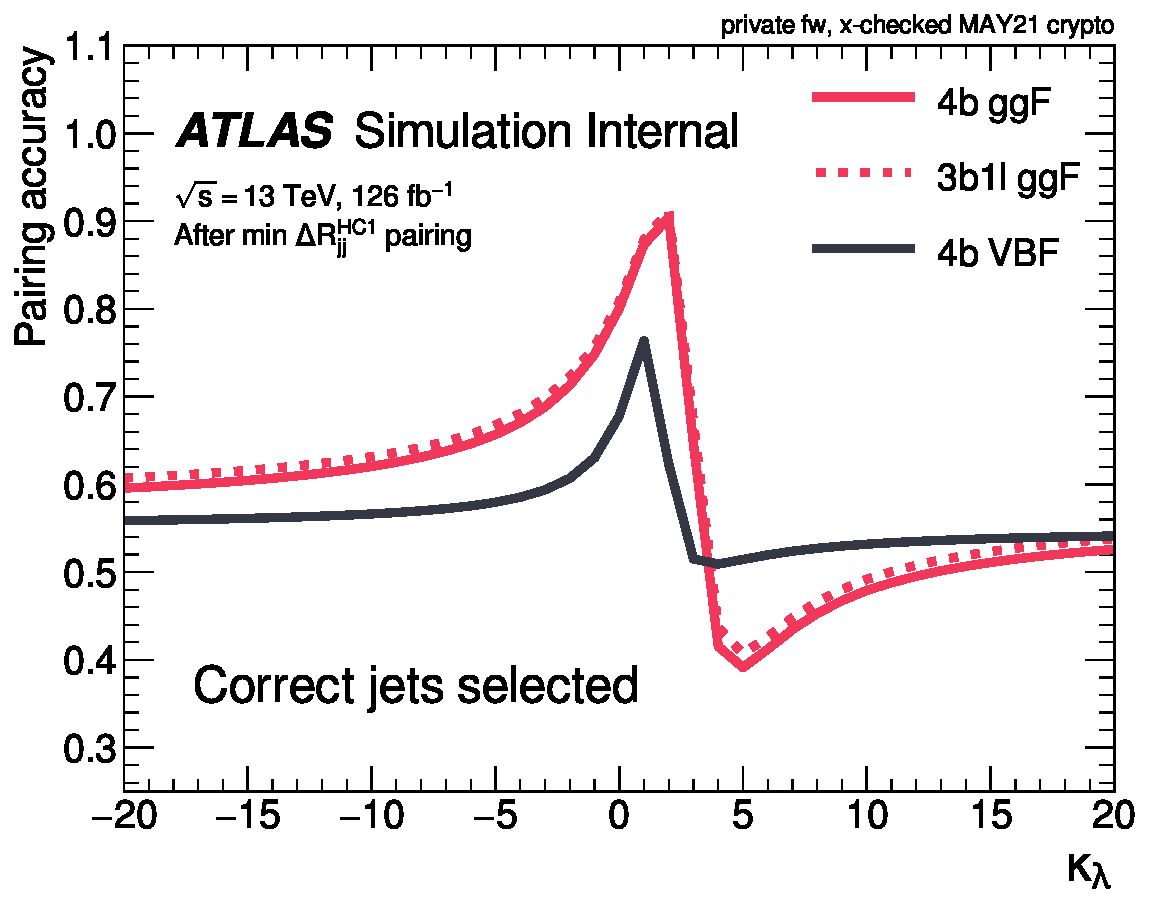
\includegraphics[width=0.4\textwidth]{selection/pairing_accuracy_kl}
                \label{fig:acc_kl_exists}
            }
            \subfloat[Pairing accuracy vs $\kappa_{2V}$]{
                     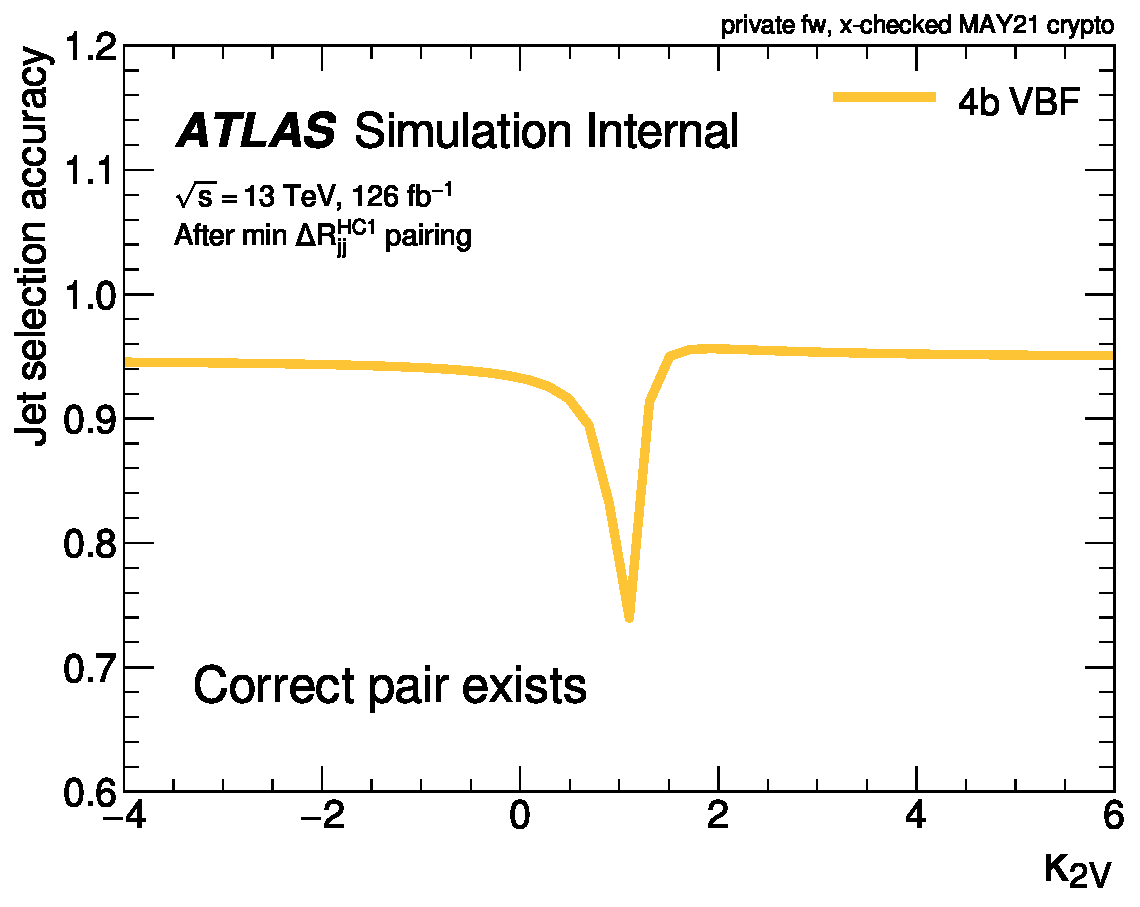
\includegraphics[width=0.4\textwidth]{selection/pairing_accuracy_k2v}
                \label{fig:acc_k2v_exists}
            }
            \caption{TODO \cite{hh4b_2021_int_note}}
            \label{fig:HHpairing}
        \end{figure}
                                                                                                         
        \FloatBarrier


    \subsection{Region Definition}
        
        There are three ``regions'' which are used for the analysis.
        The ``Control'' and ``Validation'' regions are used for the Background Estimation (see Chapter \ref{chapter:background}).
        The ``Signal'' Region is the set of data which will be used to search for the di-Higgs signal.

        The region which an event falls into is based on the reconstructed masses of the leading and sub-leading Higgs.
        The Signal Region (SR) corresponds to those events for which the reconstructed Higgs masses
            align closely with the measured value of the Higgs Boson (125 GeV), with additional room provided for error in measurment.
        The Control and Validation Regions (CR and VR) are adjacent to the Signal Region,
            designating events with kinematics very similar to the Signal Region,
            but with reconstructed Higgs masses incompatible with experimental measurment (see Figure \ref{fig:region_definition}).
        The boundaries of these regions are governed by a quantity $X_HH$, defined as:

        \begin{equation}
            X_{HH} \equiv \sqrt{\left(\frac{m_{H1} - 124\textrm{GeV}}{0.1 \ m_{H1}}\right)^{2}
                + \left(\frac{m_{H2} - 117\textrm{GeV}}{0.1 \ m_{H2}}\right)^{2}}
            \label{eq:xhh}
        \end{equation}
        
        The SR is defined by $X_{hh} < 1.6$,
            while the CR and VR are set within a ring-like shape between the Signal Region
            and an outer bondary defined by:
        \begin{equation}
            \text{CR\ Outer\ Edge} \quad : \quad \sqrt{ \left(m_{H1} - 1.05 \cdot 124\textrm{GeV}\right)^2
                +  \left(m_{H2} - 1.05 \cdot 117\textrm{GeV}\right)^2 } = 45\textrm{GeV}
            \label{eq:cr_out}
        \end{equation}
        
        The split between the CR and VR is based on studies demonstrating that this split results in
            close kinematic similarity between the two regions.

        \begin{figure}[tbh]
            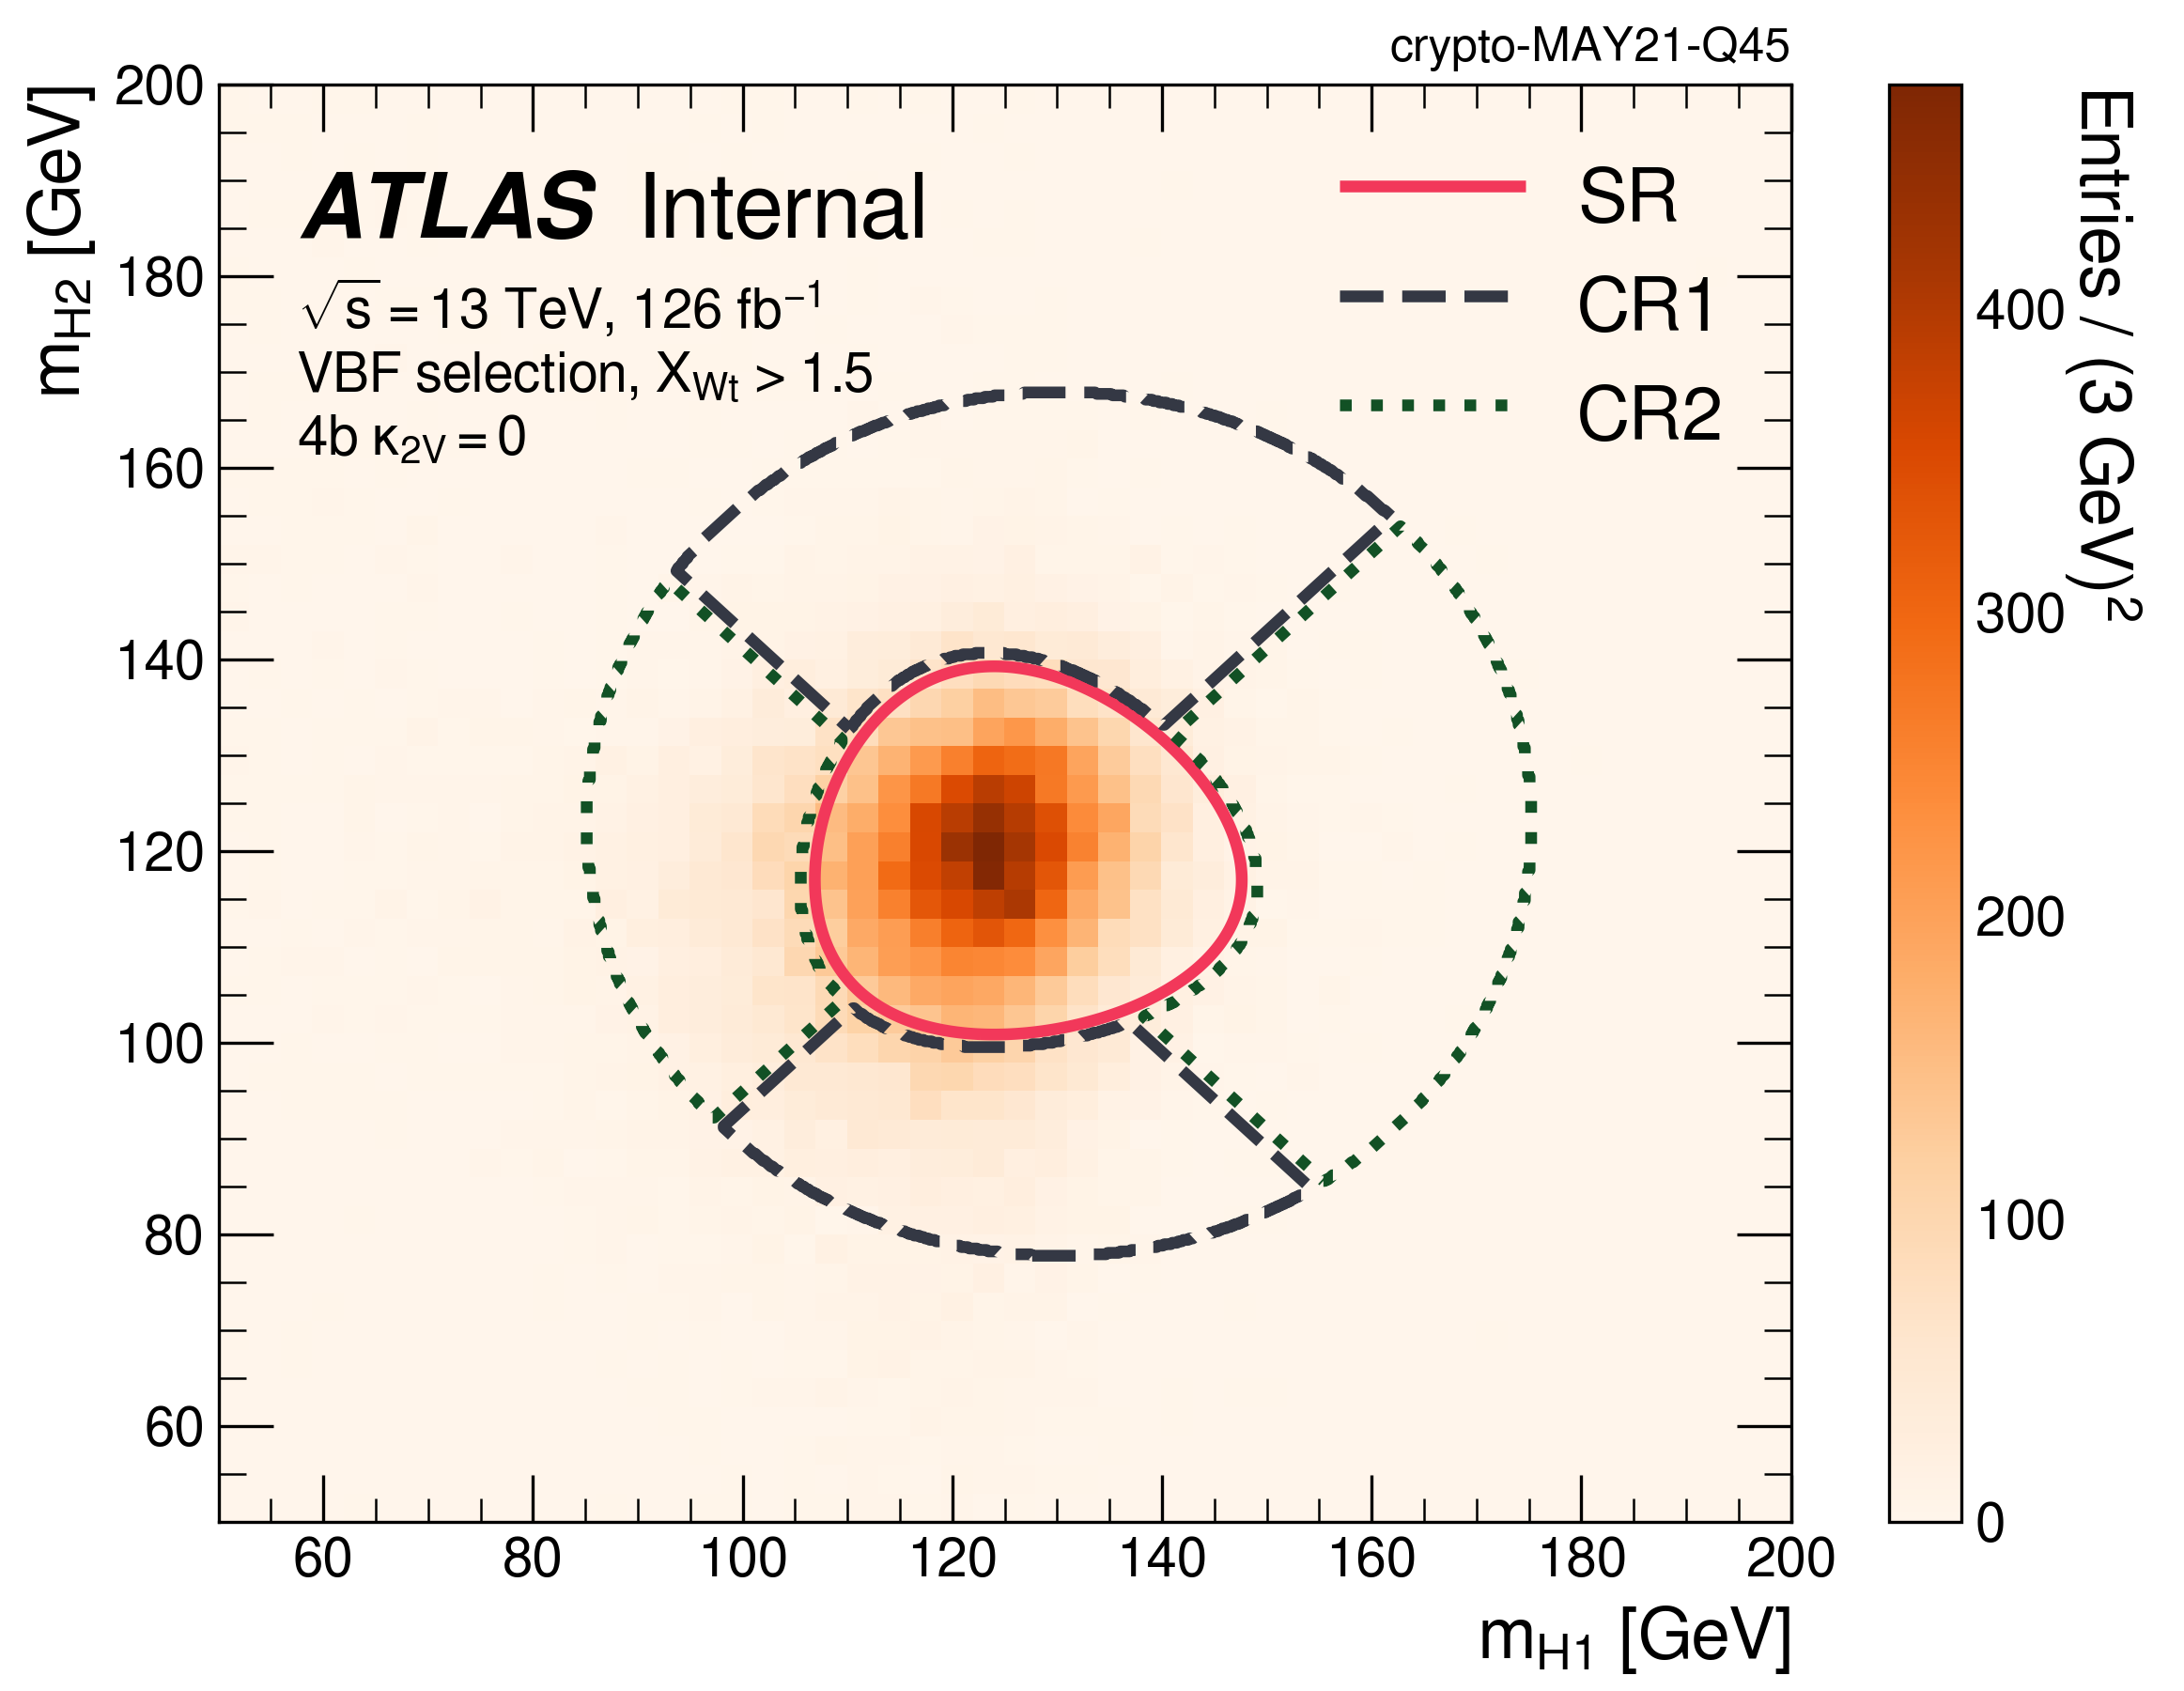
\includegraphics[width=\linewidth,height=\textheight,keepaspectratio]{selection/massplane_sig_all_4b_vbf_Xwt_1.5_k2V_0}
            \caption{
                We use k2v=0 because we're trying to exclude it.\cite{hh4b_2021_int_note}
            }
            \label{fig:region_definition}
        \end{figure}


        %Do I need to show proof of all our cut steps? Like, surely there's a motivation for each of them?

  %      Two VBF Initial Scatter (IS) quark jets:
  %          light jets (u,d, or maybe charm);
  %          high pt;
  %          wide opening angle;
  %          high mjj;
  %          can be central or forward.

  %      Four b-jets:
  %          decay products of higgss;
  %          all central; why are interesting things always central?
  %                       can i show this mathematically (dude it's just Newton's first law... don't overthink it)
  %          also high pt;
  %          b/b-bar products are expected to have very low opening angle between them.

  %      Overall:
  %          Zero pt initially, so expected low pt for vector sum of all jets combined
  %          

  %      Make note of the fact that the anti-$k_t$ algorithm is set with $\Delta R = 0.4$.

  %  kinematic cuts
  %      basic jet multiplicity reqs,
  %      btag jets with DL1r 77\% working point,
  %      4b-tagged, central
  %      also 2b and 3b1f, which are reserved for background estimation
  %      2 non-btagged jets with min-mjj for VBF

  %  Then there's the minDR pairing of b's to reconstruct HH

  %  Then cut on dihiggs and full system kinematics

  %  Then make sure the higgss fall within the "signal region" (their individual masses are approximately 125 GeV)


%...and how we wittle the abundance of events down to a manageable subset.
%If I stick to this format, there's still a bit of event reconstruction done here.
%
%HH4b Resolved Reco and Selection (literally just go through resolved recon...).
%    Final stage is the signal region selection


% Ch8: Background Estimation - DRAFT 2
\chapter{Background Modelling} \label{chapter:background}

\section{Data-Driven Background Estimate}

Selection doesn't remove all non-signal events (not even close...),
    so we need to be able to model the background (which consists of ttbar and QCD) that remains.

We need a way to predict what the kinematic shape of the background will look like in the 4b Signal region,
    without looking in the signal region.
Background simulation with MC is not feasible because the background for this many jets is absurd
    and not something we can simulate in a reasonable time-span.
Instead, we're going to predict the background in our data using *other* parts of our data.

Fundamental assumption is that background events with only 2 b-tagged jets (2b data)
    will have kinematics very similar to the background events with 4 b-tagged (4b) jets.
Thus, we can use the kinematic distribution of the 2b signal region as an estimate of the background in the 4b signal region.
Unfortunately, we can't expect the kinematics to match completely, so we have to "reweight" the 2b signal data,
    which adjusts the kinematic distribution to match that of 4b.
This reweighting takes the form of a function $R$,
    which for each event $i$ takes a series of kinematic variables $x_i$ as an argmuent,
    and returns a reweight value $r_i$ that scales that event's contribution to kinematic distributions:
    $r_i = R(x_i)$.
The set of variables used for this function are discussed in a later section
    (just copy your appendix on the VBF NNRW vars from the int note).

This reweighting function is derived using machine learning techniques.
A neural network is trained to identify how reweight 2b data such that the final result looks like 4b data.
Though, in order to improve stability in the reweighting function,
    we use not one neural network, but rather the median of 100 neural networks (which is called the "Nominal Estimate").
Note that each neural network instance $j$ produces a reweighting factor $w_{ij}$, and has a normalization factor $\alpha_j$ associated with it.
This normalization is such that the total yield of all 2b reweighted events,
    matches that of the 4b yield in the same region.
So for $N$ total 2b events and $N'$ total 4b events:
    \begin{equation}
    \sum_{i=1}^{N} \alpha_j w_{ij} = N'
    \end{equation}

The nominal estimate $\tilde{w}$ constructed from the median of these networks will not neccesarily satisfy this same relation,
    so it is given its own seperate normalization $\tilde \alpha$:
    \begin{equation}
    \sum_{i=1}^{N} \tilde \alpha \tilde w_i = N'
    \end{equation}

    TODO: include a bunch of those reweighting validation plots


\section{VBF Background Reweighting Variables} \label{app:vbf_bgdNNRW}
    The Neural Network used to reweight the 2b-Tagged Control-Region data into the 4b Signal region,
        uses a different set of variables when trained for the VBF process than it does for ggF.
    This list of variables was selected by first producing a set of plots showing how strongly correlated different variables are to \mhh
        (Figure \ref{fig:mhh_corr}).

    \begin{figure}[!htbp]
        \subfloat[$\deta \leq 1.5$]{
            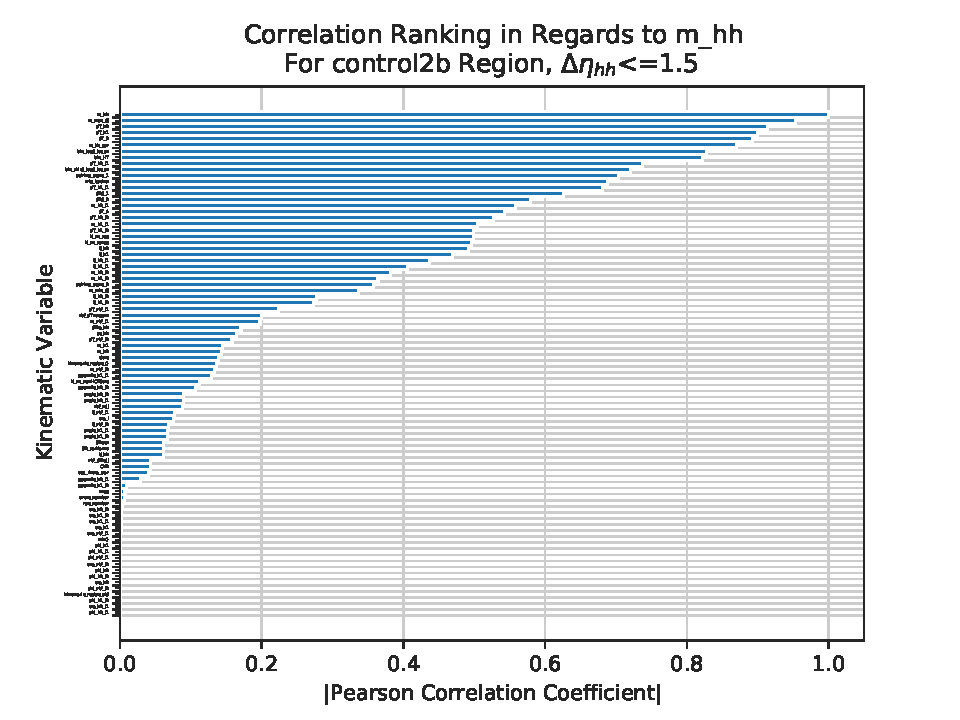
\includegraphics[width=0.5\linewidth,height=\textheight,keepaspectratio]{background/correlation_control2b_detahh-LTE1.5_hist_m_hh}
        }
        \subfloat[$\deta > 1.5$]{
            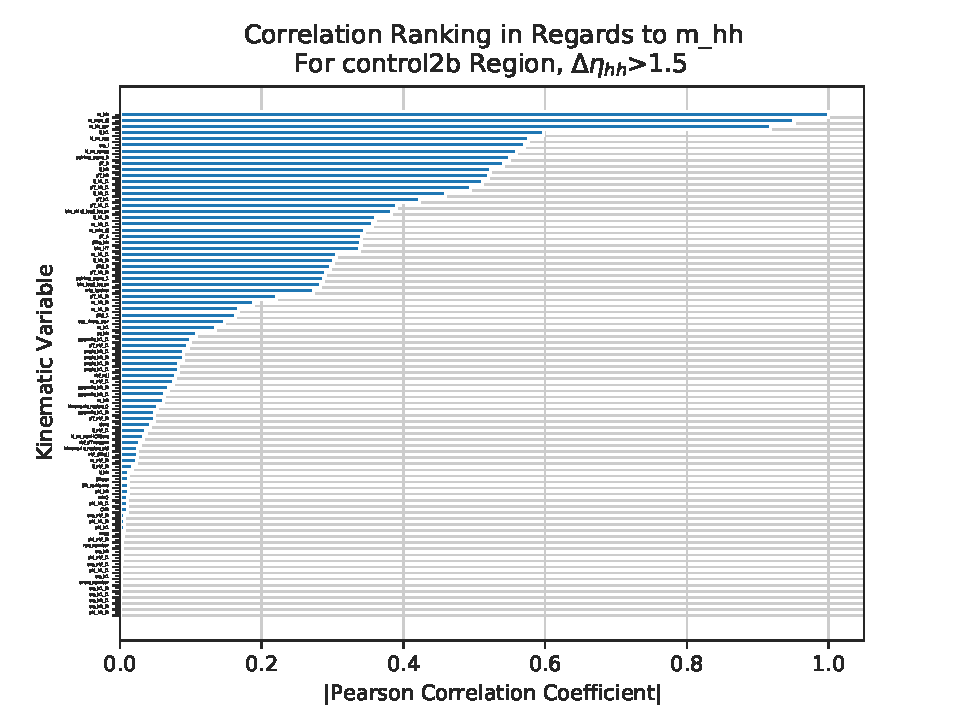
\includegraphics[width=0.5\linewidth,height=\textheight,keepaspectratio]{background/correlation_control2b_detahh-GT1.5_hist_m_hh}
        }
        \caption{
            The Pearson Correlation Coefficients associated with \mhh for the 2b Control Region data.
            The regions in which $\deta \leq 1.5$ and $\deta>1.5$ are separately displayed.
            The higher up on the chart a variable is, the more strongly correlated it is to \mhh,
                with \mhh itself at the top with a coefficient of 1.
            Note that most of the VBF-specific variables, such as vbf\_mjj, are very poorly correlated to \mhh and thus not preffered.
        }
        \label{fig:mhh_corr}
    \end{figure}

    Based on their high correlation to \mhh in both \deta regions, 23 variables were then selected for further study.
    These 23 variables were plotted against each other in a correlation matrix.
    A final set of seven variables was selected based (Table \ref{tab:vbf_NNRW_vars}) on which variables were \textit{least} correlated to each other,
        in order to avoid variables carrying redundant information (Figure \ref{fig:vbf_corr_matrix}).

    \begin{figure}[!htbp]
        \subfloat[$\deta \leq 1.5$]{
            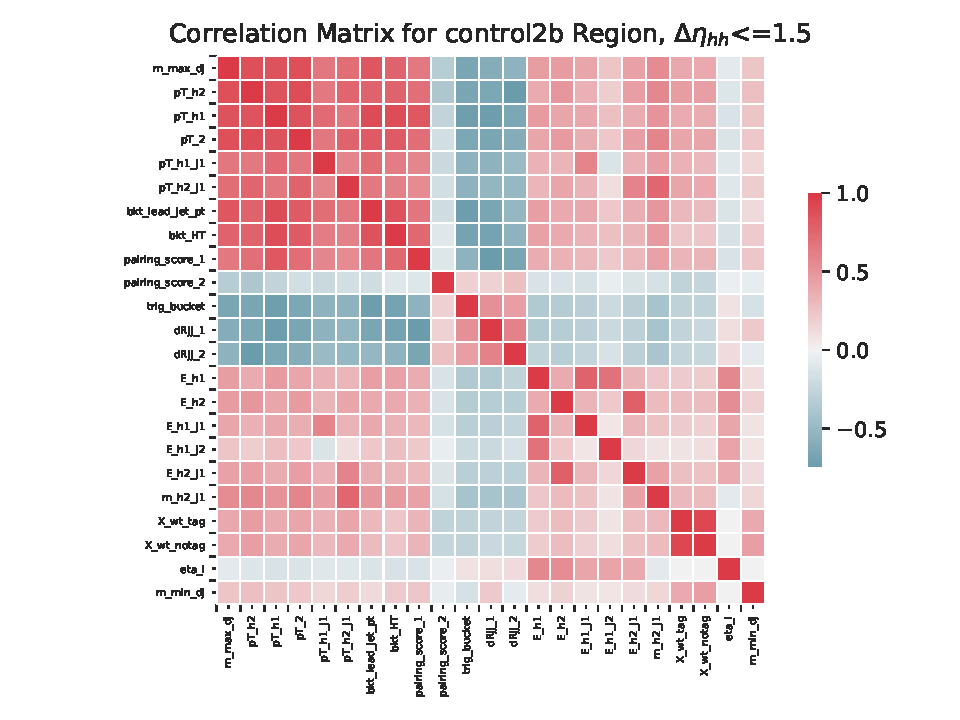
\includegraphics[width=0.5\linewidth,height=\textheight,keepaspectratio]{background/correlation_control2b_detahh-LTE1.5_matrix}
        }
        \subfloat[$\deta > 1.5$]{
            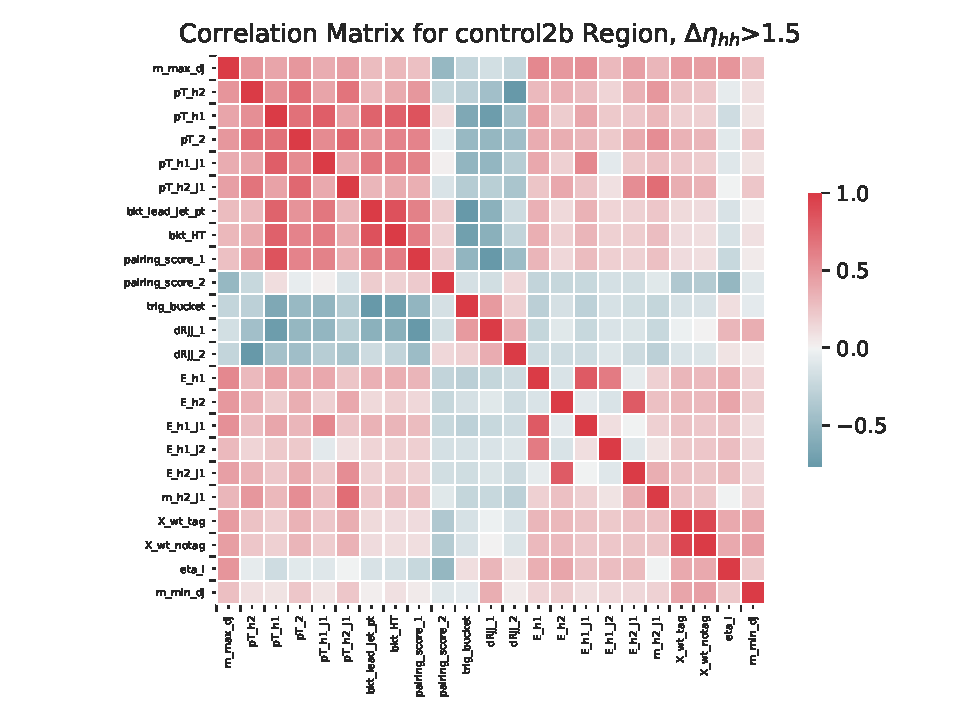
\includegraphics[width=0.5\linewidth,height=\textheight,keepaspectratio]{background/correlation_control2b_detahh-GT1.5_matrix}
        }
        \caption{
            The Pearson Correlation Coefficients matrix associated with variables in the 2b Control Region data.
            The regions in which $\deta \leq 1.5$ and $\deta>1.5$ are separately displayed.
            Bins with more saturated (i.e.\ more blue or more red) colors indicate strong correlation between those two variables.
            All variables are of course 100\% correlated to themselves, hence the deep red line running down the diagonal.
            The most highly preffered variables are those with correlation coefficients near 0 for as many other variables as possible.
            If a variable (i.e.\ m\_max\_dj) is selected, any other variables with strong correlations to it (i.e.\ pT\_h2)
                are then strongly disfavored for later selection.
        }
        \label{fig:vbf_corr_matrix}
    \end{figure}


    %'m_max_dj', 'E_h1', 'E_h2', 'X_wt_tag', 'm_min_dj', 'eta_i', 'pairing_score_2' 
    \begin{table}[!htbp] \centering \footnotesize
    \caption{Final Set of Neural Network Variables}
    \label{tab:vbf_NNRW_vars}
    \begin{tabular}{ |l|l|l| }
        \hline
        \textbf {Variable} & \textbf {Internal Name} & \textbf {Description} \\
        \hline
        $M_{max \Delta j}$ & \code{m\_max\_dj}         & 
            Take the di-jet mass of the six possible pairings\\
            && of the four higgs’ candidate jets;\\
            && this is the maximum di-jet mass of those pairings \\ 
        \hline
        $M_{min \Delta j}$ & \code{m\_min\_dj}         & 
            As above, but the minimum \\
        \hline
        $E_{H1}$           & \code{E\_h1}              & 
            Energy of the leading-$p_T$ reconstructed Higgs \\
        \hline
        $E_{H2}$           & \code{E\_h2}              & 
            Energy of the sub-leading-$p_T$ reconstructed Higgs \\
        \hline
        Xwt-tag            & \code{X\_wt\_tag}         & 
            $\log\left(X_{Wt}\right)$, where $X_{Wt}$ is the variable used for the top veto \\
        \hline
        $\eta_i$           & \code{eta\_i}             & 
            Average $\eta$ of the the four Higgs decay jets \\
        \hline
        Pairing Score 2    & \code{pairing\_score\_2 } & 
            This changes depending on the Higgs pairing algorithm used. \\
            &&The current algorithm used is minDR. \\
            &&With four jets, there are three possible pairings of the jets. \\
            &&The pairings are ranked by the $\Delta_R$ of the leading-$p_T$ Higgs candidate. \\
            &&Pairing Score 2 is the $\Delta-R$ of the second-smallest of these pairings. \\
        \hline
    \end{tabular} \end{table}


\section{Systematic Error}

The problem with this training approach, is that the 4b signal region cannot be used to train against.
Instead, the Neural networks must be trained on the Control region (4b Cr?).
Because the reweighting function is trained on a different kinematic region than the signal region,
    a systematic uncertainty is associated with it.
This is calculated by training another ensemble of NNs on yet another kinematic region (Validation);
    the difference between the median of these validation-trained NNs and the nominal estimate
    is used to compute the overall background estimation systematic uncertainty.
The precise formula for this error is:
    $what?$.


The region difference error is combined with a additional errors resulting from a lot of things.

\section{Statistical Error}

Now to talk about statistical error in the Neural network estimate

Poisson stat errors: stat error on bin i is 
    \begin{equation}
    \sigma_i = \sqrt{\sum_{j \in i} w_j^2}
    \end{equation}

Bootstrap uncertainty: A bin-by-bin statistical error resulting from the variations in each of the networks' reweighting functions.
Naively, this would mean using the average of all networks, with an error calculated as the standard deviation of all histograms of all the networks, for a given variable of interest.
Slightly less naively (to make us more robust to outliers),
    we would use the median of all networks, and the IQR values of the networks as the error.
In reality, it's impractical to retain the information of all networks for all histograms.
We can still use the median value, but the error has to be calculated another way.
Specifically, the error is calculated by storing a small amount of extra information regarding the IQR of the bootstraps.
Whenever a kinematic distribution is produced, \textbf{two} histograms are generated:
    the nominal histogram, and the \textit{varied} histogram.
The difference between the values of the nominal and varied histograms, per bin,
    are taken as the error on that bin for the nominal histogram.

The nominal event weights are calculated as
    \begin{equation}
    \tilde w_i = \textrm{median}(\alpha_1 w_{1,i}, ..., \alpha_{100} w_{100,i})
    \end{equation}
    with the normalization $\tilde \alpha$ calculated as described above.
So if the yield of normalized nominal weights is denoted
    \begin{equation}
    \tilde Y \equiv \sum_{i=1}^{N} \tilde \alpha \tilde w_i = \textrm{yield of 4b control region}
    \end{equation}
then the values of the bins of the nominal histogram, $H_j$ are:
    \begin{equation}
    H_j = \tilde \alpha \sum_{i \in j} \tilde w_i
    \end{equation}

A "weight variation" factor is calculated per event as 
    \begin{equation}
    V^w_i = \frac{1}{2}\textrm{IQR}(w_{1,i}, w_{2,i}, ..., w_{100,i})
    \end{equation}
Likewise, a "normalization variation" factor is calculated as
    \begin{equation}
    V^{\alpha} = \frac{1}{2}\textrm{IQR}(\alpha_{1}, \alpha_{2}, ..., \alpha_{100})
    \end{equation}
The sum of the varied weights is 
    \begin{equation}
    Y_v = \sum_{i=1}^{N} \left( \tilde w_i + V^w_i \right)
    \end{equation}
And the ratio of the nominal yield to the varied yield is $R_Y \equiv \tilde Y / Y_v$

The "varied" histogram $H'$ is then calculated based on these variation factors as:
    \begin{equation} \begin{split}
    H'_j &= \left[ R_Y \sum_{i \in j} \tilde w_i + V^w_i \right] + V^{\alpha} H_j
    \\H'_j &= \sum_{i \in j} \left[ R_Y \left( \tilde w_i + V^w_i \right)
        + V^{\alpha} \tilde \alpha \tilde w_i \right]
    \end{split} \end{equation}

The error of the nominal histogram bin $j$ then is
    \begin{equation} \begin{split}
    \sigma_j &= | H'_j - H_j |
    \\&= \left| \sum_{i \in j} \left[
        R_Y \left( \tilde w_i + V^w_i \right)
        + V^{\alpha} \tilde \alpha \tilde w_i \right] 
        -\tilde \alpha \sum_{i \in j} \tilde w_i \right|
    \\&= \left| \sum_{i \in j} \left[
        R_Y \left( \tilde w_i + V^w_i \right)
        + V^{\alpha} \tilde \alpha \tilde w_i 
        - \tilde \alpha \tilde w_i
        \right] \right|
    \\&= \left| \sum_{i \in j} \left[
        R_Y \left( \tilde w_i + V^w_i \right) 
        + \tilde \alpha \tilde w_i (V^{\alpha}-1) \right] \right|
    \end{split} \end{equation}



% Ch9: Signal Modeling - DRAFT 2
\chapter{Signal Modeling} \label{chapter:signal}

\section{Building a Hypothesis}

    The core of the scientific method is in the practice of making a hypothesis
        and of then testing that hypothesis through experiment.
    The hypothesis made in this analysis is that the Standard Model of Particle Physics is mostly correct
        and that deviations from this theory should manifest in the probabilities of physical processes.
    I have spent the past several chapters discussing the experimentation process.
    Now it is time to discuss how I constructed a hypothesis that can be tested against the data provided from that experiment.

    The most basic hypothesis made in this analysis is that the di-Higgs process exists at all.
    Unfortunately, a direct measurement of the di-Higgs process is unlikely to occur in this study, as will be discussed in Chapter \ref{chapter:results}.
    An additional hypothesis that can be tested, however,
        is related to the Higgs Boson coupling scaling factors and their influence on di-Higgs production cross-sections
        (c.f. Eqn. \ref{eq:tree_level_invamp}).
    If the Standard Model is exactly correct, then the various $\kappa$ scaling factors,
        discussed in Section \ref{sec:higgs_boson},
        should all be identically 1.
    A simple hypothesis to construct would be to calculate the expected event yield of the \vbfproc process
        by multiplying the integrated luminosity of LHC Run 2 with the cross-section predicted by the SM.
    The same could be done to obtain predicted event yields for various alternative values of the scale factor.
    However, testing a hypothesis using a single number presents a challenge, as many different unrelated factors can affect the event yield.


    \begin{figure}[tbh]
        \centering
        \begin{subfigure}{0.48\textwidth}
            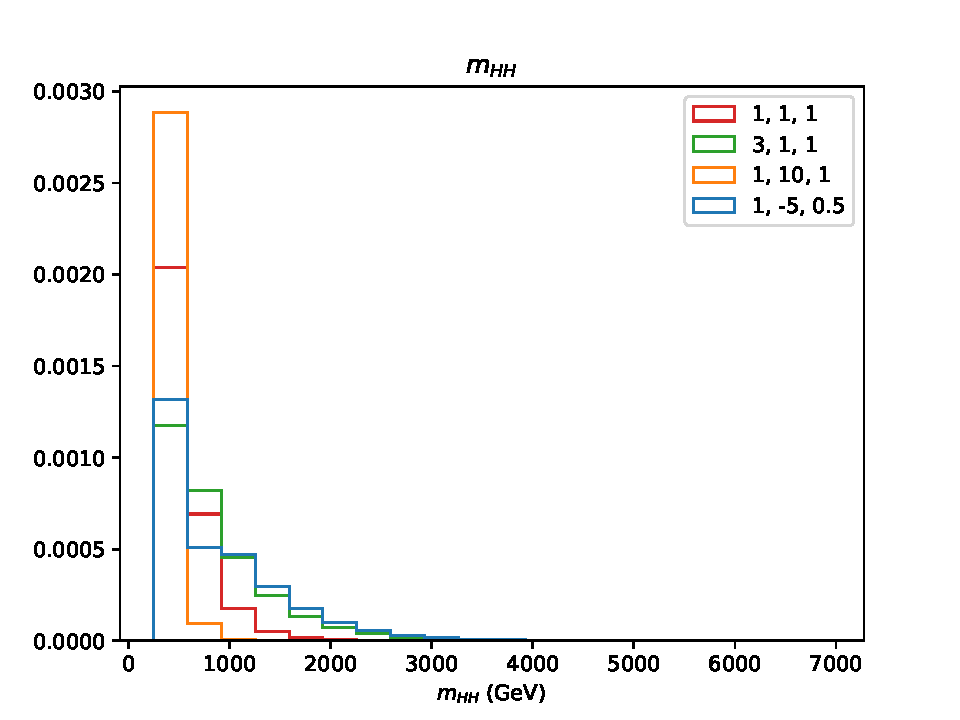
\includegraphics[width=\linewidth,height=\textheight,keepaspectratio]{signal/truth_lhe_HH_m}
            \captionsetup{justification=centering} \caption{Di-Higgs Invariant Mass}
        \end{subfigure}
        \begin{subfigure}{0.48\textwidth}
            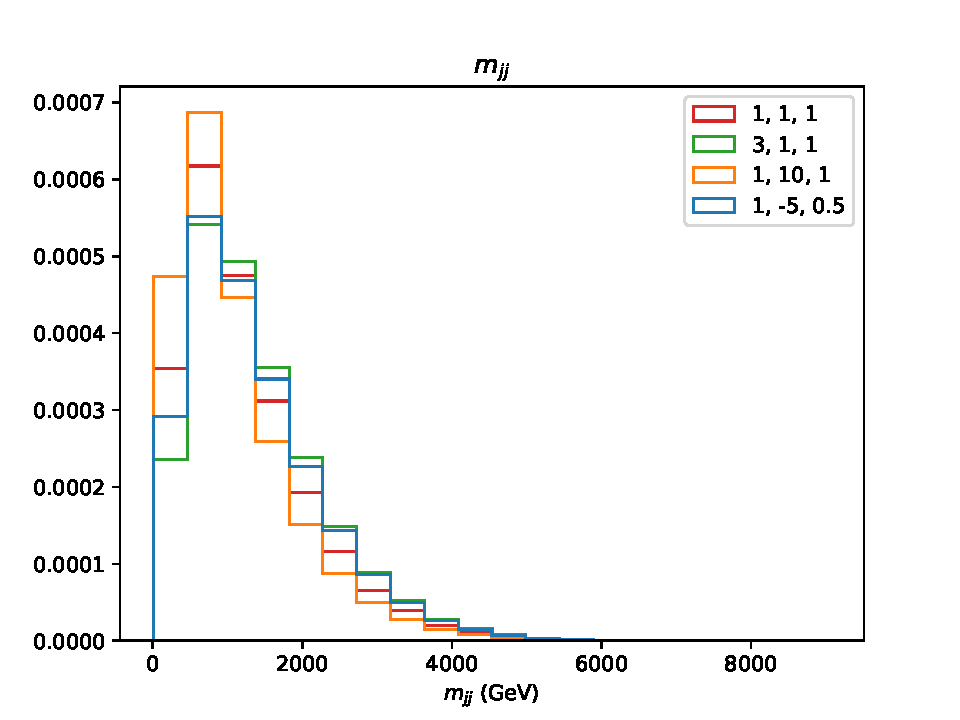
\includegraphics[width=\linewidth,height=\textheight,keepaspectratio]{signal/truth_lhe_jj_M}
            \captionsetup{justification=centering} \caption{VBF Initial Scatter Jets Invariant Mass}
        \end{subfigure}
        \caption{
            MC event distributions from \textit{truth-level} events.
            That is, events generated from MadGraph+Pythia8
                but which have not gone through Geant4 detector simulation or reconstruction.
            These plots show the invariant mass between the Higgs pair and VBF initial scatter jets respectively,
                for a number of different $\kappa$ scale factors.
        }
        \label{fig:lhe_truth1}
    \end{figure}

    \begin{figure}[tbh]
        \centering
        \begin{subfigure}{0.48\textwidth}
            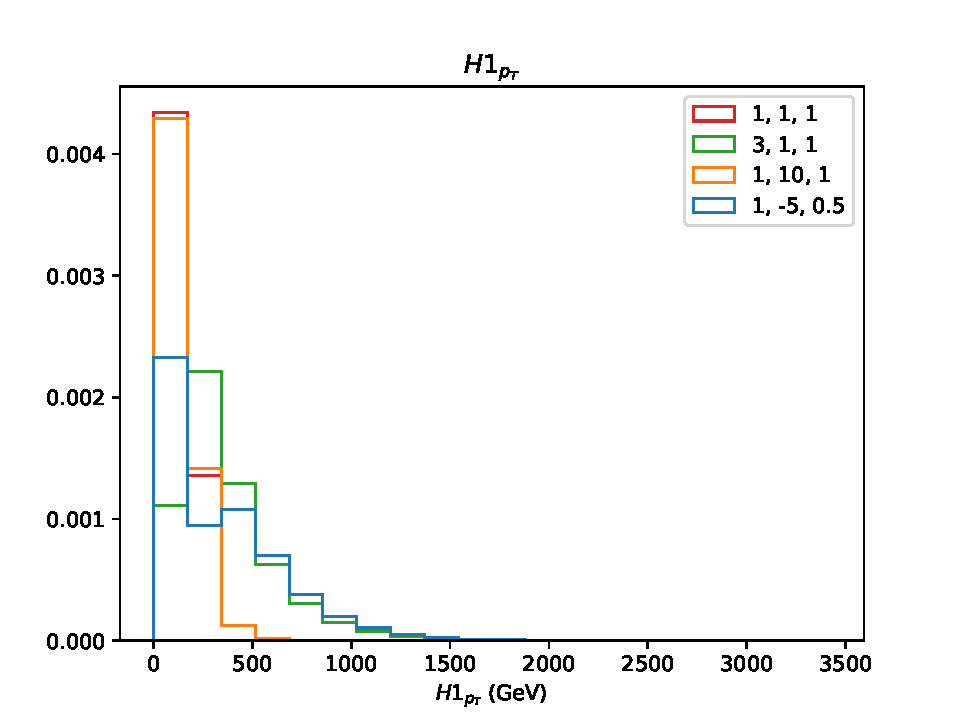
\includegraphics[width=\linewidth,height=\textheight,keepaspectratio]{signal/truth_lhe_H1_pt}
            \captionsetup{justification=centering} \caption{
                $p_T$ of the leading-$p_T$ Higgs boson
            }
        \end{subfigure}
        \begin{subfigure}{0.48\textwidth}
            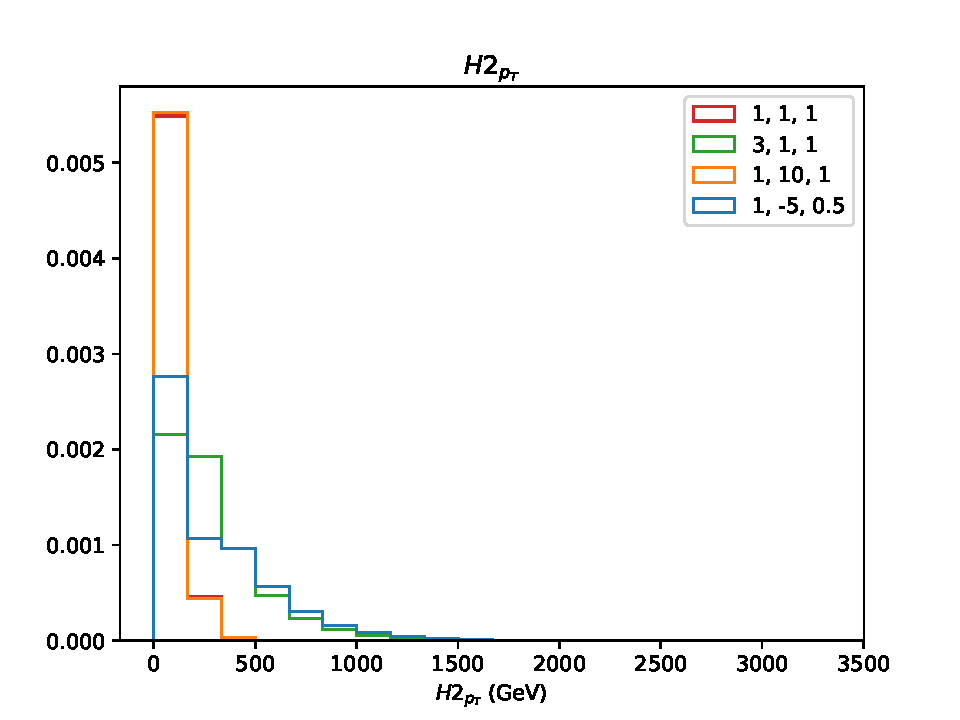
\includegraphics[width=\linewidth,height=\textheight,keepaspectratio]{signal/truth_lhe_H2_pt}
            \captionsetup{justification=centering} \caption{
                $p_T$ of the sub-leading-$p_T$ Higgs boson
            }
        \end{subfigure} \\

        \begin{subfigure}{0.48\textwidth}
            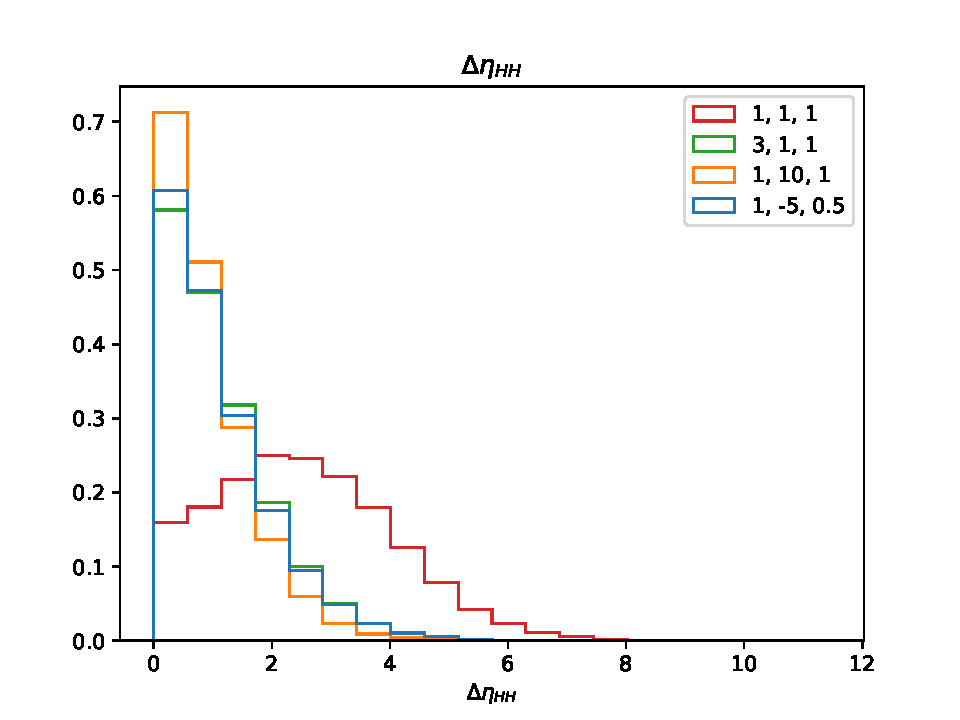
\includegraphics[width=\linewidth,height=\textheight,keepaspectratio]{signal/truth_lhe_HH_dEta}
            \captionsetup{justification=centering} \caption{
                \deta between the two produced Higgs bosons
            }
        \end{subfigure} \\
        \caption{
                Truth-level display of additional kinematic properties the \vbfhhproc.
        }
        \label{fig:lhe_truth2}
    \end{figure}

    Instead, a more robust hypothesis can be constructed by choosing an observable quantity distinct to the process in question.
    Here, the observable used is the invariant mass of the di-Higgs system (\mhh).
    The advantage of using \mhh is that the probability density function (PDF) for the \mhh of an event
        is predicted to vary significantly based on the values of the $\kappa$ scaling factors.
    As such, the shape of the PDF for \mhh is unique to particular values of the scale factors, 
        and so can be used to test the validity of a hypothesis.
    If the \mhh distribution reconstructed from the data collected at ATLAS has no resemblance to
        the \mhh distribution predicted for a particular combination of the scale factors,
        then that set of scale factors can be ruled out as incompatible with data
        at some level of statistical confidence
        (to be further discussed in Chapter \ref{chapter:results}).

    Of course, making a prediction for the shape of the \mhh distribution as it would appear in ATLAS is easier said than done.
    Calculating the event yield alone is not too difficult to perform by hand,
        as this requires only the cross-section of the process.
    Calculating the event yield as a function of an observable kinematic variable is much more difficult,
        requiring the differential cross-section $\dxsec{q_i}$.
    Section \ref{sec:mcsim} describes the Monte-Carlo simulation procedure used for this purpose,
        providing a model of how the kinematic distributions of the \vbfhhproc process would appear after passing through
        the ATLAS detector and the event selection process.
    The challenge addressed in this chapter then is with regard to the poorly defined range of the kappa coupling coefficients,
        and the variety of signal hypotheses this range entails.
    Modelling such a range accurately and efficiently necessitates revisiting the fundamental behaviour
        of the \hhproc process, and constitutes the bulk of my contribution to the 4b analysis.


\section{Signal Combination} \label{sec:signal_combination}

    As discussed in Section \ref{sec:feyn_rules},
        the cross-section and kinematic distributions of the di-Higgs production processes
        depend fundamentally on a number of scaling factors between the Higgs and other particles.
    Of particular interest in this analysis are \kl for the Higgs's self-coupling scale factor and \kvv for the \HHVV coupling scale factor.
    The values of \kl and \kvv have loose experimental constraints \cite{EXOT-2016-31} \cite{HDBS-2018-18-witherratum} \cite{ATLAS-CONF-2019-049},
        requiring analysis across a wide range of these scale factor values.
    Unfortunately, the MC generation process discussed in Section \ref{sec:mcsim} is computationally expensive and time consuming.
    As such, only a handful of MC simulation samples for a select few scale factor values are actually produced.
    A sample combination technique 
        (expanded upon from an analogous approach used in Ref. \cite{combination_origin})
        is employed to model the signal hypothesis across the scale factor parameter space.

    The process of combining a few samples in such a way as to model the entire parameter space of scaling factors
        is based on exploiting the underlying mathematics of the differential cross-section formula.
    By expanding the squared term of the sum of all Feynman diagram contributions,
        the cross-section can be expressed as a function of its scale factor values \cite{ATLAS-CONF-2019-049},
        as shown in Eqn. \ref{eq:tree_level_invamp}.
    Rewriting the expression again in terms of the differential cross-section as a function of the observable \mhh:
    \begin{equation} \begin{split} \label{eq:tree_level_invamp_simple}
        \xsec &\equiv \dXsecM \propto |\invAmp|^2 = |  \kv^2 M_t + \kv \kl M_s + \kvv M_x |^2 \\
        \xsec &= \kv^2 \kl^2 a_1 + \kv^4 a_2 + \kvv^2 a_3 + \kv^3 \kl a_4 + \kv \kl \kvv a_5 + \kv^2 \kvv a_6
        \,.
    \end{split} \end{equation}

    \newcommand{\crossterm}[1]{
        \xsec_{#1} &= \fkv{#1}^2 \fkl{#1}^2 a_1
            + \fkv{#1}^4 a_2
            + \fkvv{#1}^2 a_3
            + \fkv{#1}^3 \fkl{#1} a_4
            + \fkv{#1} \fkl{#1} \fkvv{#1} a_5
            + \fkv{#1}^2 \fkvv{#1} a_6
    }
    %\newcommand{\combterm}[1]{ g_{#1} \frac{d\sigma_{#1}}{d \mhh} }
    \newcommand{\combterm}[1]{ g_{#1} \xsec_{#1} }

    The $a_i$ matrix element expansion values have a dependence on \mhh, which is not trivially derivable as an analytic function.
    Instead, for a given scale factor,
        its cross-section for a given \mhh can be mathematically determined by solving a set of linear equations for the $a_i$ terms.
    This is done using six different cross-section values (for the same \mhh) for six different scaling values.

    %\begin{equation} \label{eq:allsixxsecs} \begin{aligned}
    %\begin{equation} \crossterm{1} \nonumber \end{equation}
    %\begin{equation} \crossterm{2} \nonumber \end{equation}
    %\begin{equation} \crossterm{3} \nonumber \end{equation}
    %\begin{equation} \crossterm{4} \nonumber \end{equation}
    %\begin{equation} \crossterm{5} \nonumber \end{equation}
    %\begin{equation} \label{eq.allsixxsecs} \crossterm{6} \,. \end{equation}
    %\end{aligned} \end{equation}

    \begin{eqnarray} \label{eq:allsixxsecs}
        \crossterm{1} \nonumber \\
        \crossterm{2} \nonumber \\
        \crossterm{3} \nonumber \\
        \crossterm{4} \nonumber \\
        \crossterm{5} \nonumber \\
        \crossterm{6} \nonumber \,. \\
    \end{eqnarray}

    This set of equations can be reformatted as a matrix equation
        by rewriting the differential cross-sections and $a_i$ terms as vectors,
    \begin{equation}
        \vec{\xsec} = \minimatrix{ \xsec_{1} \\ \xsec_{2} \\ \xsec_{3} \\ \xsec_{4} \\ \xsec_{5} \\ \xsec_{6} }
        \qquad,\qquad
        \vec{a} = \minimatrix{ a_1 \\ a_2 \\ a_3 \\ a_4 \\ a_5 \\ a_6 }
        \,.
    \end{equation}
    By reformatting the various $\kappa$ terms as a vector function $\vec{f}$,
        the collection of varied scale factors can be written as a matrix $F$
    \begin{equation}
        \vec{f} = \begin{pmatrix} \kv^2 \kl^2 \\ \kv^4 \\ \kvv^2 \\ \kv^3 \kl \\ \kv \kl \kvv \\ \kv^2 \kvv \end{pmatrix}
        \quad,\quad
        F = \begin{pmatrix}
            \vec{f}(\fkvv{1}, \fkl{1}, \fkv{1}) \\
            \vec{f}(\fkvv{2}, \fkl{2}, \fkv{2}) \\
            \vec{f}(\fkvv{3}, \fkl{3}, \fkv{3}) \\
            \vec{f}(\fkvv{4}, \fkl{4}, \fkv{4}) \\
            \vec{f}(\fkvv{5}, \fkl{5}, \fkv{5}) \\
            \vec{f}(\fkvv{6}, \fkl{6}, \fkv{6}) \\
        \end{pmatrix}
        \,.
    \end{equation}

    Equation \ref{eq:allsixxsecs} can then be written in the much simpler form
    \begin{equation}
        \vec{\xsec} = F \bullet \vec{a}
        \,.
    \end{equation}
    The $a_i$ terms can then be trivially solved for through an inversion of $F$
    \begin{equation} \label{eq:amp_solution}
        \vec{a} = F^{-1} \bullet \vec{\xsec}
        \,.
    \end{equation}
    Substituting \ref{eq:amp_solution} back into \ref{eq:tree_level_invamp_simple} produces
        a final expression for deriving a combined differential cross-section $\xsec'$ of the form
    \begin{equation} \label{eq:combination_general} \begin{split}
        \xsec'(\kvv,\kl,\kv) &= \vec{f}(\kvv,\kl,\kv) \bullet \vec{a}
            = \vec{f}(\kvv,\kl,\kv) \bullet F^{-1} \bullet \vec{\xsec} \\
        \xsec'(\kvv,\kl,\kv) &= \vec{g}(\kvv,\kl,\kv) \bullet \vec{\xsec}
            \quad,\quad \vec{g} \equiv \vec{f}(\kvv,\kl,\kv) \bullet F^{-1} \\
        \xsec'(\kvv,\kl,\kv) &= 
            \combterm{1} +
            \combterm{2} +
            \combterm{3} +
            \combterm{4} +
            \combterm{5} +
            \combterm{6}
        \,.
    \end{split} \end{equation}

    In practice, the differential cross-section values $\xsec_i$ of these six \textit{basis} samples
        are represented by their yields from MC simulation,
        binned by their \mhh values,
        which are added together after being multiplied by their respective combination coefficient $g_i$.
    Due to the complexities of the kinematics of the VBF process,
        the samples used in the combination must have already been run through the full reconstruction and selection process detailed in Section \ref{sec:mcsim}.
    The signal distribution modeling is thus performed by directly combining the reconstructed \mhh distributions of post-selection signal samples.

    \begin{table}[] \centering
    \caption{6-Term VBF Combination Sample Variations.}
    \label{tab:vbf_hh_6term_varlist}
    \begin{tabular}{ |l|l|l| }
        \hline
        \textbf {$\kappa_{2V}$} & \textbf {$\kappa_\lambda$} & \textbf {$\kappa_V$} \\
        \hline
            1   &   1 & 1   \\
            1.5 &   1 & 1   \\
            1   &   2 & 1   \\
            1   &  10 & 1   \\
            1   &   1 & 0.5 \\
            0   &  -5 & 0.5 \\
        \hline
    \end{tabular} \end{table}

    In theory, with infinite events, the only requirement for these samples is that they are linearly independent of each other.
    In practice, the final samples are statistically limited, and different combinations of variations yield different statistical power.
    The 6-sample combination used in this analysis (Table \ref{tab:vbf_hh_6term_varlist} and Eqn. \ref{eqn:vbf_hh_6term_chosen}) has been chosen specifically for its ability to avoid mis-modeling errors.

    {\footnotesize \begin{equation}
    \label{eqn:vbf_hh_6term_chosen}
    \begin{split}
        \xsec'(\kvv, \kl, \kv) =
        \left(\frac{68 \kappa_{2V}^{2}}{135} - 4 \kappa_{2V} \kappa_{V}^{2} + \frac{20 \kappa_{2V} \kappa_{V} \kappa_{\lambda}}{27} + \frac{772 \kappa_{V}^{4}}{135} - \frac{56 \kappa_{V}^{3} \kappa_{\lambda}}{27} + \frac{\kappa_{V}^{2} \kappa_{\lambda}^{2}}{9}\right)
            \times & \xsec{\left(1,1,1 \right)} \\
        + \left(- \frac{4 \kappa_{2V}^{2}}{5} + 4 \kappa_{2V} \kappa_{V}^{2} - \frac{16 \kappa_{V}^{4}}{5}\right)
            \times & \xsec{\left(\frac{3}{2},1,1 \right)} \\
        + \left(\frac{11 \kappa_{2V}^{2}}{60} + \frac{\kappa_{2V} \kappa_{V}^{2}}{3} - \frac{19 \kappa_{2V} \kappa_{V} \kappa_{\lambda}}{24} - \frac{53 \kappa_{V}^{4}}{30} + \frac{13 \kappa_{V}^{3} \kappa_{\lambda}}{6} - \frac{\kappa_{V}^{2} \kappa_{\lambda}^{2}}{8}\right)
            \times & \xsec{\left(1,2,1 \right)} \\
        + \left(- \frac{11 \kappa_{2V}^{2}}{540} + \frac{11 \kappa_{2V} \kappa_{V} \kappa_{\lambda}}{216} + \frac{13 \kappa_{V}^{4}}{270} - \frac{5 \kappa_{V}^{3} \kappa_{\lambda}}{54} + \frac{\kappa_{V}^{2} \kappa_{\lambda}^{2}}{72}\right)
            \times & \xsec{\left(1,10,1 \right)}  \\
        + \left(\frac{88 \kappa_{2V}^{2}}{45} - \frac{16 \kappa_{2V} \kappa_{V}^{2}}{3} + \frac{4 \kappa_{2V} \kappa_{V} \kappa_{\lambda}}{9} + \frac{152 \kappa_{V}^{4}}{45} - \frac{4 \kappa_{V}^{3} \kappa_{\lambda}}{9}\right)
            \times & \xsec{\left(1,1,\frac{1}{2} \right)} \\
        + \left(\frac{8 \kappa_{2V}^{2}}{45} - \frac{4 \kappa_{2V} \kappa_{V} \kappa_{\lambda}}{9} - \frac{8 \kappa_{V}^{4}}{45} + \frac{4 \kappa_{V}^{3} \kappa_{\lambda}}{9}\right)
            \times & \xsec{\left(1,-5,\frac{1}{2} \right)}
        \,.
    \end{split} \end{equation}}

    The method used to determine the overall performance of a basis is to check the number of negative bins generated
        in the \mhh distribution across all points in the two-dimensional \kvv,\kl space, as seen in Fig. \ref{fig:vbf_hh_6term_nWeight_grid}.
    As negative bin weights are unphysical, they indicate poor signal modeling.
    Thus, identifying a basis which minimizes the presence of negative weights
        ensures stable modeling of the signal hypothesis at all points in the coupling space
        (Figs. \ref{fig:vbf_hh_6term_validation} and \ref{fig:vbf_hh_6term_preview}).

    \begin{figure}[tbh]
        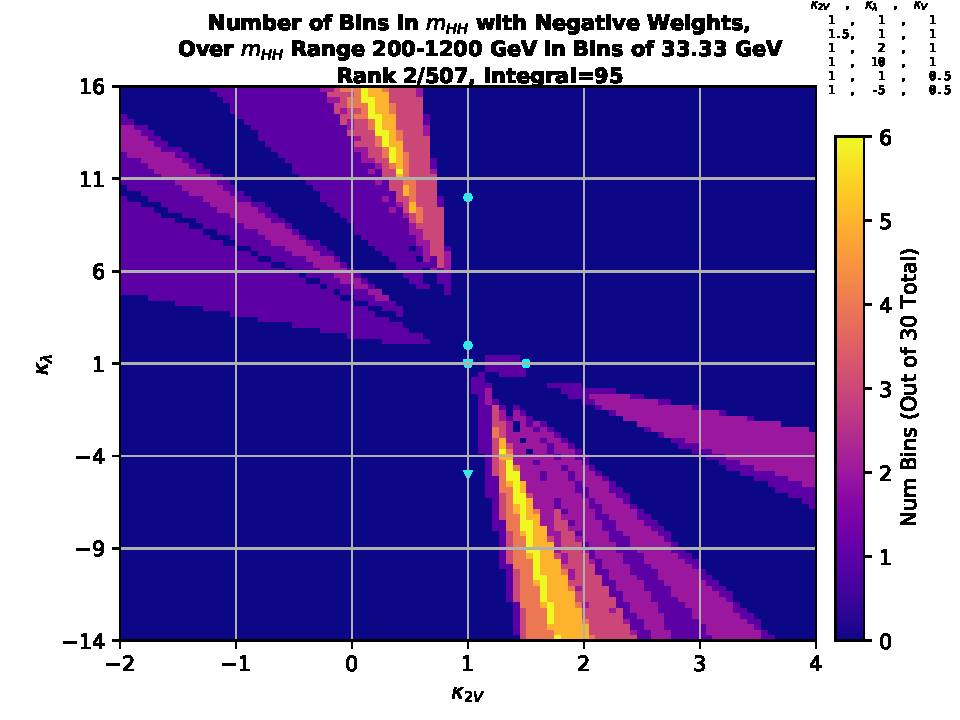
\includegraphics[width=\linewidth,height=\textheight,keepaspectratio]{signal/negative_weights_base}
        \caption{
            Frequency of negative bin weights in \mhh distribution across \kvv,\kl range.
            Brighter regions indicate more negative-weighted bins, and suggest less stable signal modeling.
            This particular combination of samples was chosen for how much of the space is ``dark,''
                with darker regions indicating generally stable signal modeling.
            The table of coupling values in the upper right corner indicates the 6 MC samples
                (highlighted on the plot with cyan dots) used in the combination.
        }
        \label{fig:vbf_hh_6term_nWeight_grid}
    \end{figure}

    Ultimately however, the final arbiter of a well constructed basis is that it produces observable distributions comparable to what would be produced through direct MC generation.
    A number of validation tests are thus performed, comparing the distributions from the combination to an already existing MC sample.
    Displayed in Fig. \ref{fig:vbf_hh_6term_validation}, the combination shows strong agreement with the MC sample.

    \begin{figure}[tbh]
        \begin{subfigure}{0.48\textwidth}
            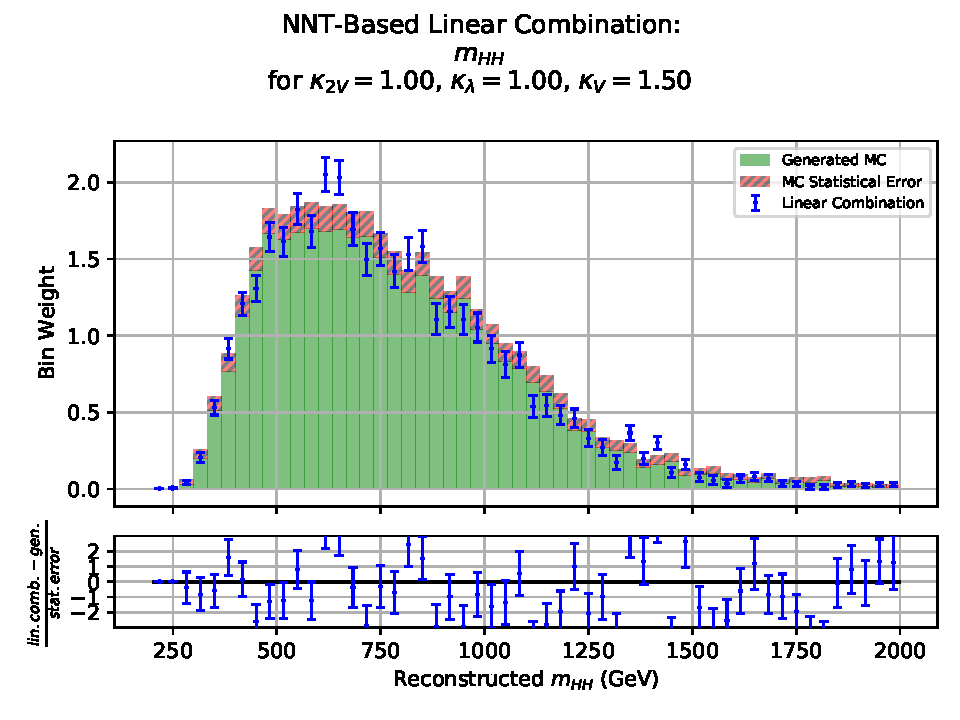
\includegraphics[width=\linewidth,height=\textheight,keepaspectratio]{signal/reco_mHH_cvv1p00cl1p00cv1p50}
            \captionsetup{justification=centering} \caption{Validation \kv = 1.5}
        \end{subfigure}
        \begin{subfigure}{0.48\textwidth}
            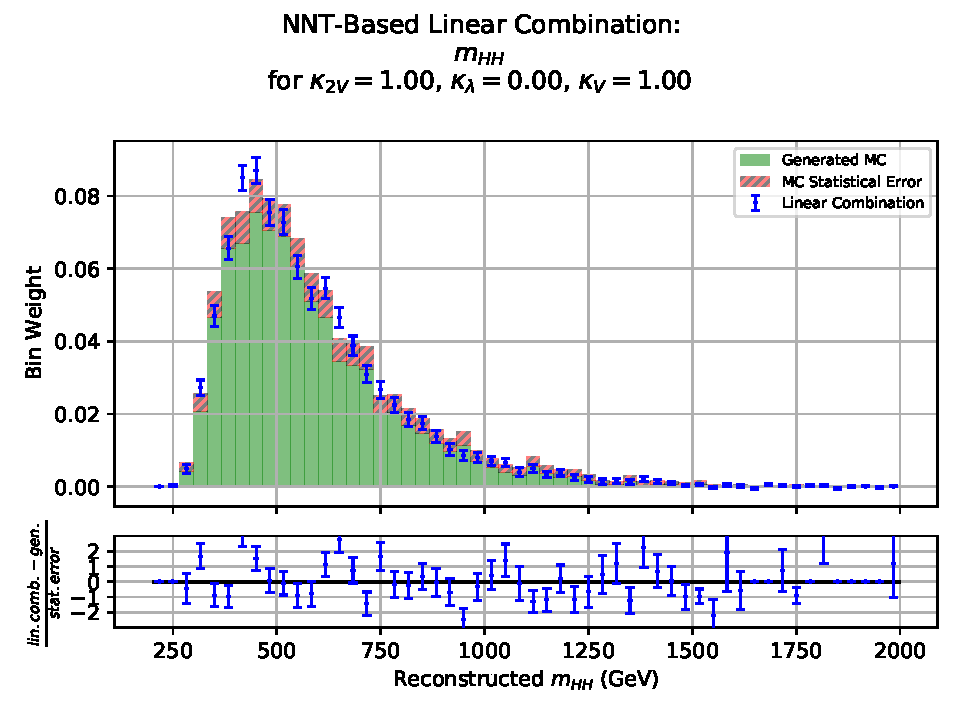
\includegraphics[width=\linewidth,height=\textheight,keepaspectratio]{signal/reco_mHH_cvv1p00cl0p00cv1p00}
            \captionsetup{justification=centering} \caption{Validation \kl = 0}
        \end{subfigure}
        \caption{
            Validation of 6-term combination against MC generated at \kv = 1.5 and \kl = 0.
            The combination shows good agreement to the generated MC distributions.
        }
        \label{fig:vbf_hh_6term_validation}
    \end{figure}

    \begin{figure}[tbh]
    	\centering
        \begin{subfigure}{0.32\textwidth}
            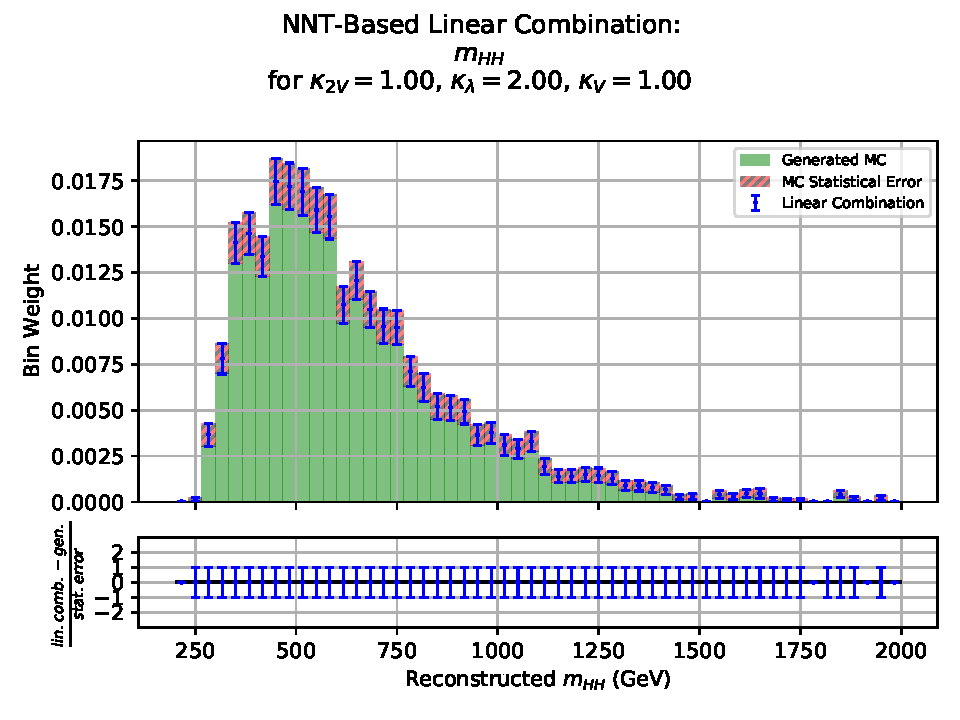
\includegraphics[width=\linewidth,height=\textheight,keepaspectratio]{signal/reco_mHH_cvv1p00cl2p00cv1p00}
            \captionsetup{justification=centering} \caption{Validation against MC with $\kl=2$}
        \end{subfigure}
        \begin{subfigure}{0.32\textwidth}
            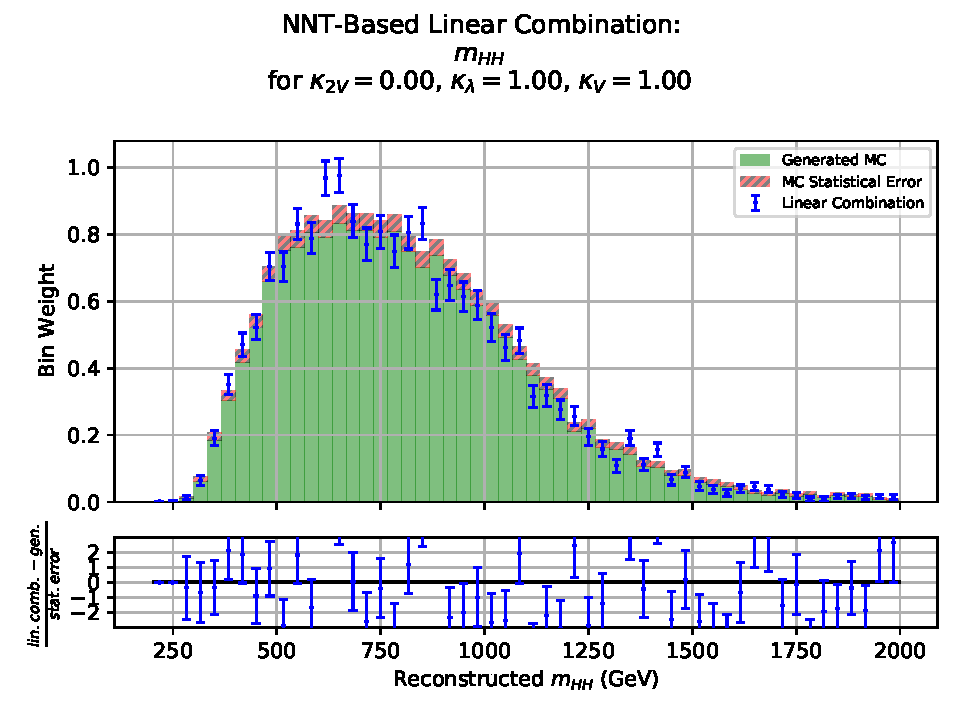
\includegraphics[width=\linewidth,height=\textheight,keepaspectratio]{signal/reco_mHH_cvv0p00cl1p00cv1p00}
            \captionsetup{justification=centering} \caption{Validation against MC with $\kvv=0$}
        \end{subfigure}
        \begin{subfigure}{0.32\textwidth}
            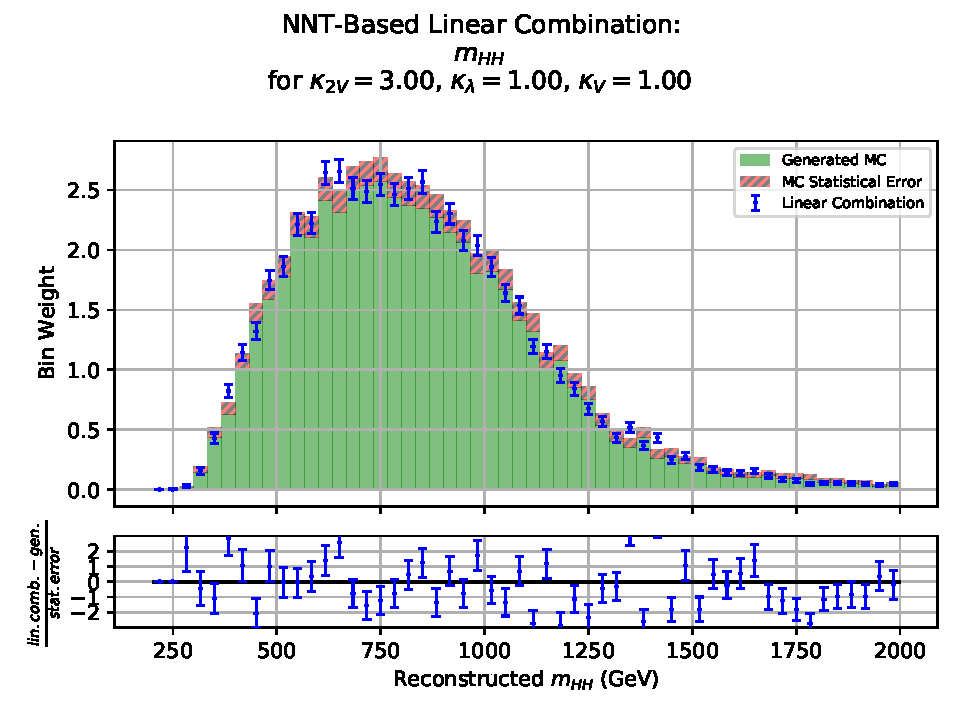
\includegraphics[width=\linewidth,height=\textheight,keepaspectratio]{signal/reco_mHH_cvv3p00cl1p00cv1p00}
            \captionsetup{justification=centering} \caption{Validation against MC with $\kvv=3$}
        \end{subfigure}
        \caption{
            The six-term linear combination of samples is combined for various coupling scaling factor values.
            The combined distribution shape (in blue) is compared against a Monte-Carlo sample (in green)
                which was generated for the same coupling scaling factor values.
            The combination approach shows good agreement with the generated sample, indicating accurate modeling of the signal shape.
        }
        \label{fig:vbf_hh_validation}
    \end{figure}

    As an additional test, I also checked the distribution shape predicted by the combination at points far from the SM.
    These points have no MC samples to compare to, but the points can still be checked to ensure they at least appear well-behaved.

    \begin{figure}[tbh]
        \centering
        \begin{subfigure}{0.32\textwidth}
            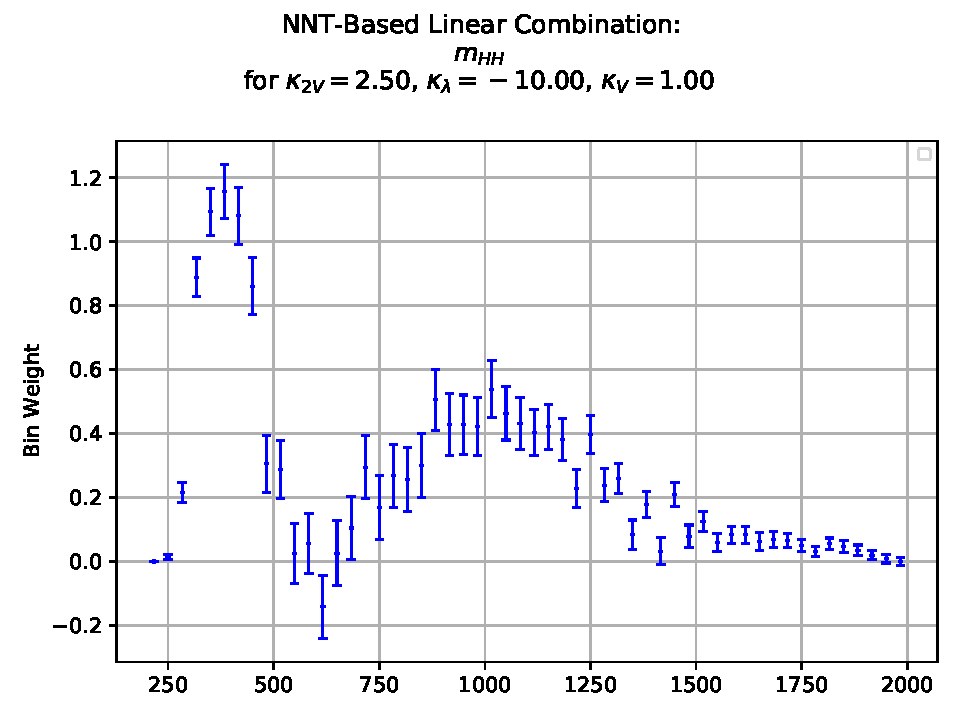
\includegraphics[width=\linewidth,height=\textheight,keepaspectratio]{signal/preview_reco_mHH_new_cvv2p50cl-10p00cv1p00}
            \captionsetup{justification=centering} \caption{Combined \mhh distribution at \kvv = 2.5, \kl = -10}
        \end{subfigure}
        \begin{subfigure}{0.32\textwidth}
            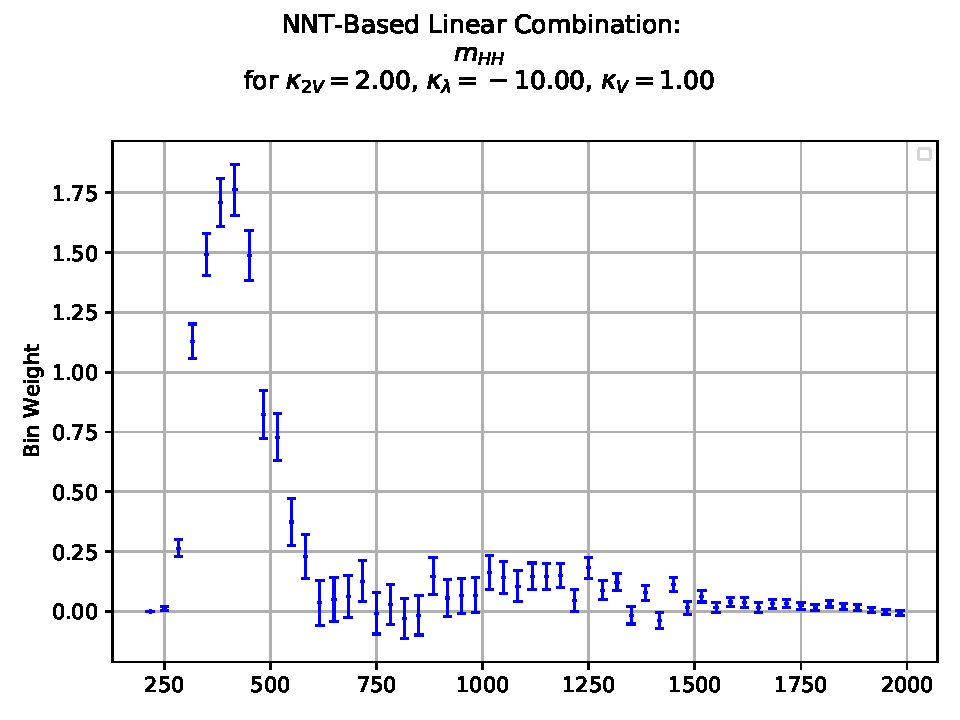
\includegraphics[width=\linewidth,height=\textheight,keepaspectratio]{signal/preview_reco_mHH_new_cvv2p00cl-10p00cv1p00}
            \captionsetup{justification=centering} \caption{Combined \mhh distribution at \kvv = 2.0, \kl = -10}
        \end{subfigure}
        \begin{subfigure}{0.32\textwidth}
            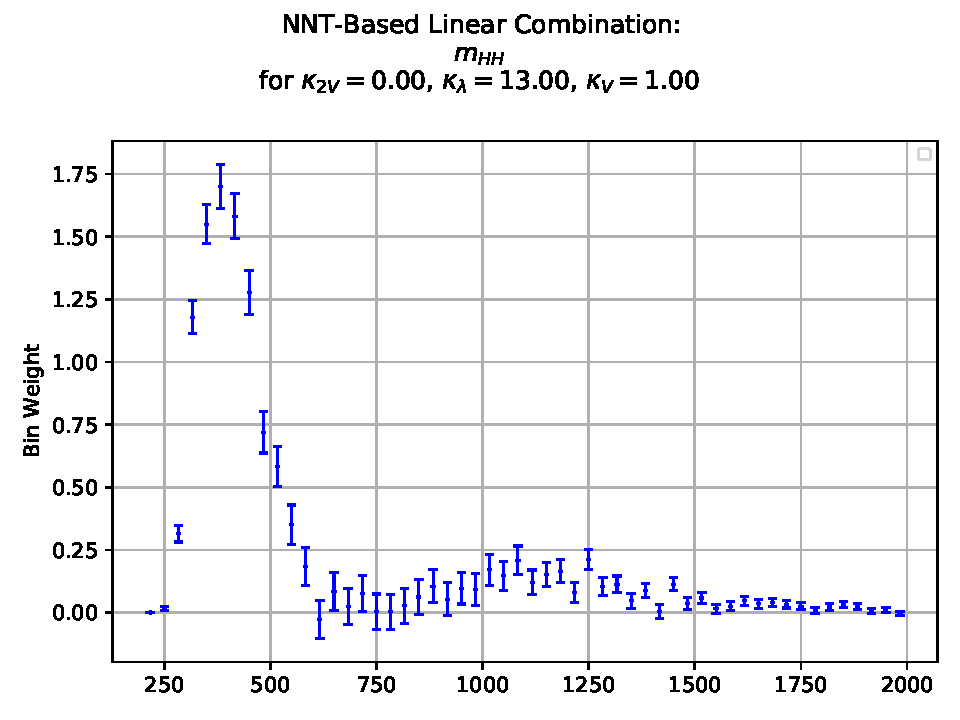
\includegraphics[width=\linewidth,height=\textheight,keepaspectratio]{signal/preview_reco_mHH_new_cvv0p00cl13p00cv1p00}
            \captionsetup{justification=centering} \caption{Combined \mhh distribution at \kvv = 0, \kl = 13}
        \end{subfigure}
        \caption{
            \mhh distribution produced by the 6-term combination at points far from the SM.
            The combination produces smooth, well-behaved distributions at these points,
                suggesting the signal is well-modeled in these regions.
        }
        \label{fig:vbf_hh_6term_preview}
    \end{figure}

    \begin{figure}[tbh]
    	\centering
        \begin{subfigure}{0.44\textwidth}
            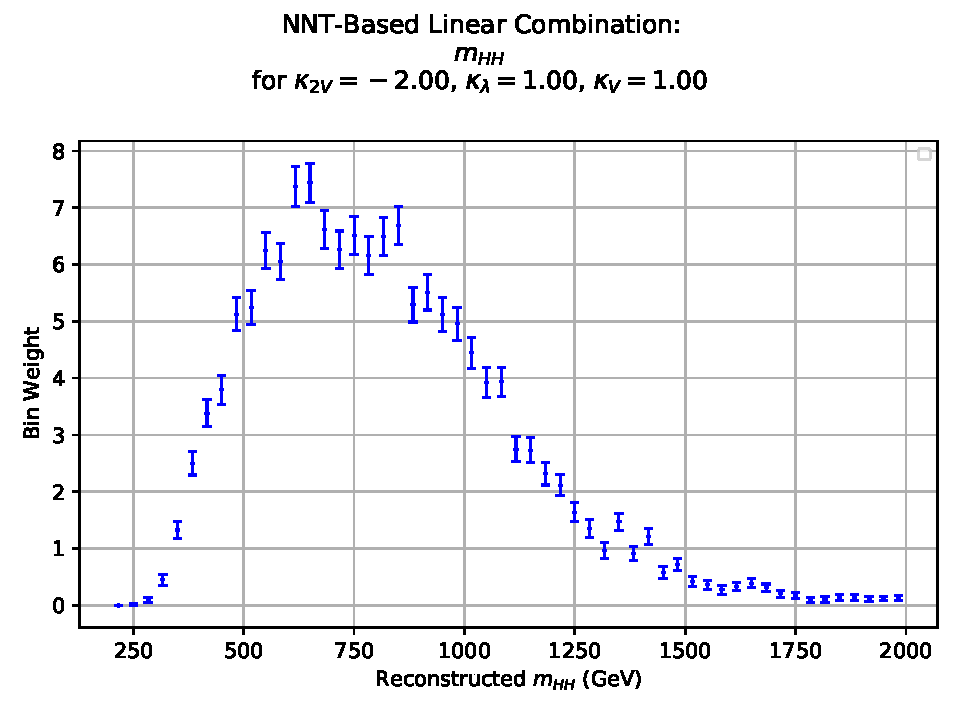
\includegraphics[width=\linewidth,height=\textheight,keepaspectratio]{signal/preview_reco_mHH_new_cvv-2p00cl1p00cv1p00}
            \captionsetup{justification=centering} \caption{Combination at  \kvv = -2}
        \end{subfigure}
        \begin{subfigure}{0.44\textwidth}
            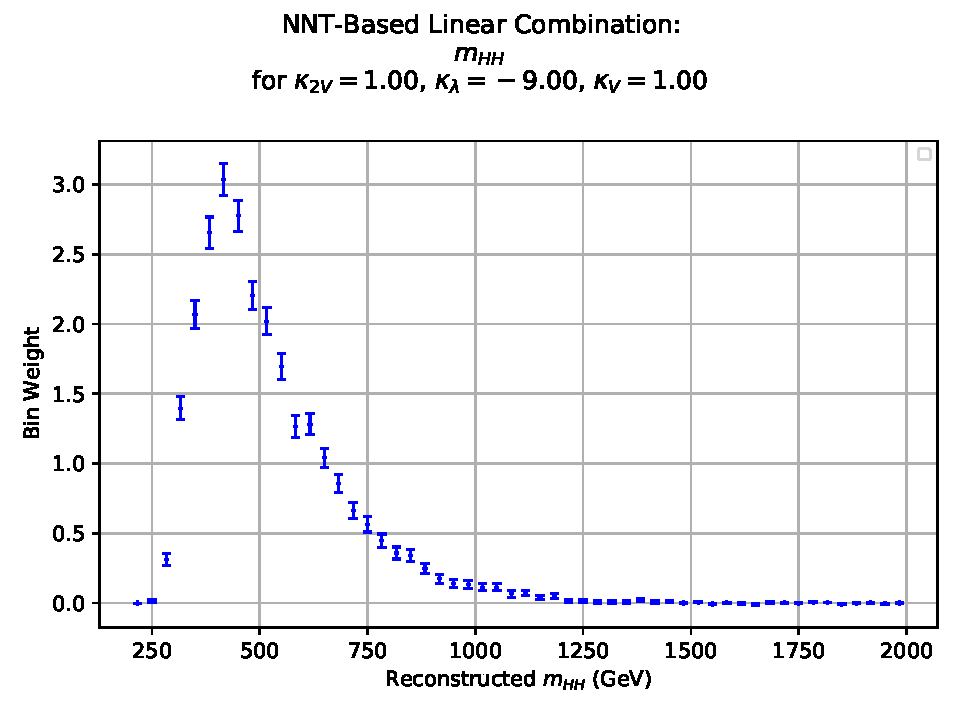
\includegraphics[width=\linewidth,height=\textheight,keepaspectratio]{signal/preview_reco_mHH_new_cvv1p00cl-9p00cv1p00}
            \captionsetup{justification=centering} \caption{Combination at  \kl = -9}
        \end{subfigure}
        \caption{
            The six-term linear combination of samples is combined for scale factor scaling factor values very far from the Standard Model.
            There are no MC simulated samples to compare these points too, but the combined distributions at these points are smooth and well-behaved,
                indicating reasonable modeling of the distribution even at distant scale factor scaling factors.
        }
        \label{fig:vbf_hh_preview}
    \end{figure}


\section{Solidarity} \label{sec:solidarity}
    
    As an additional note on the discussion of the signal sample combination technique,
        I would like to address the reason that some combination bases work better than others.
    Originally, the 2021 MC production for the 4b analysis consisted of 12 samples (all but the bottom row of Table \ref{tab:mcyields}).
    However, inspection of these samples using the negative weight technique discussed above revealed very poor modeling performance.
    From a combinatorics perspective, there were 12 samples available, and six are needed for the combination.
    There are 924 ways to choose 6 samples from 12, and of those 619 produce linearly solvable systems of equations.
    Of the 619, only 250 include the Standard Model MC sample.
    None of these 250 combination bases produced stable signal models across the $\kappa$-scale factor space.
    The performance of the two bases with the overall fewest number of negative bin weights is shown in Fig. \ref{fig:mcnWeight_old} and \ref{fig:mcpreviews_old}.

    \begin{figure}[tbh]
    	\centering
        \begin{subfigure}{0.44\textwidth}
            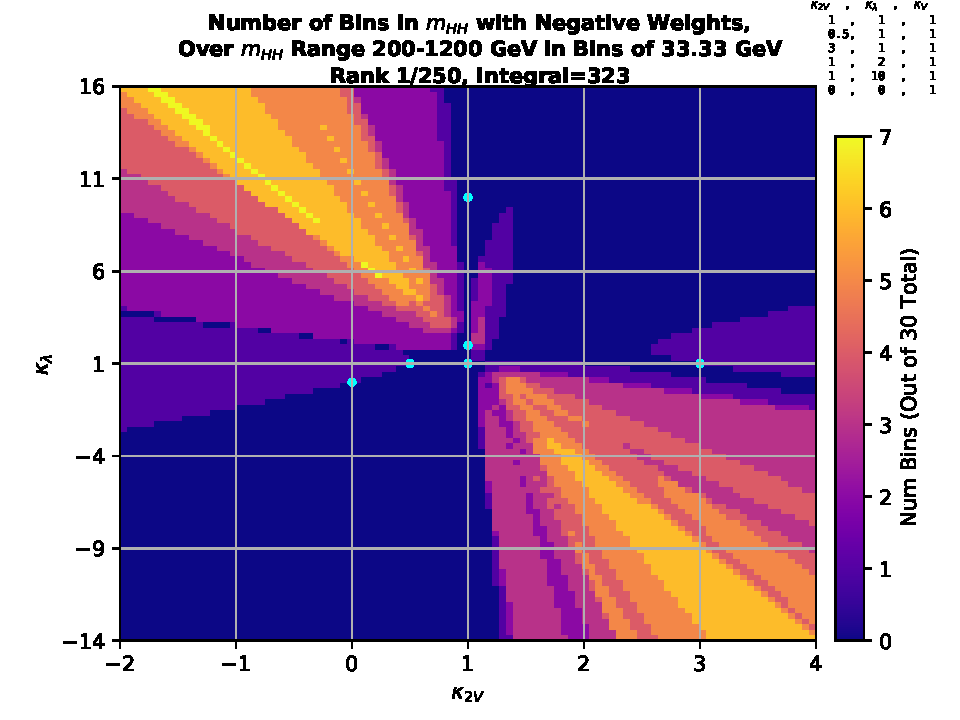
\includegraphics[width=\linewidth,height=\textheight,keepaspectratio]{signal/negative_weights_toprank0}
            \captionsetup{justification=centering} \caption{Original 12, Rank 1 negative weight heatmap}
        \end{subfigure}
        \begin{subfigure}{0.44\textwidth}
            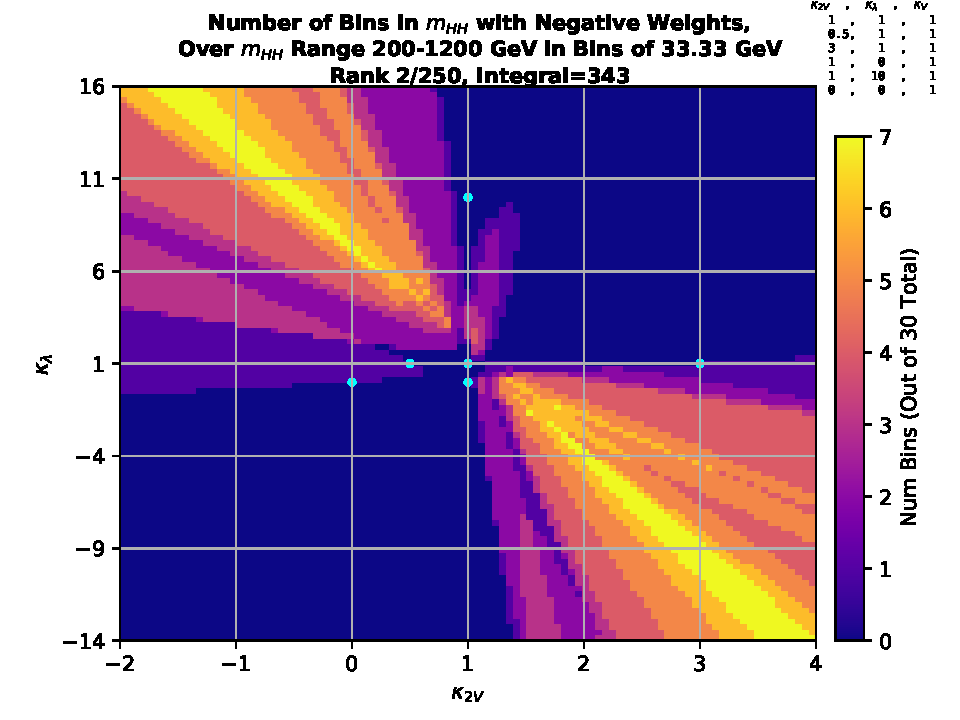
\includegraphics[width=\linewidth,height=\textheight,keepaspectratio]{signal/negative_weights_toprank1}
            \captionsetup{justification=centering} \caption{Original 12, Rank 2 negative weight heatmap}
        \end{subfigure}
        \caption{
            The two best performing bases of the original 12 MC samples.
            Both bases show a distressing abundance of negative weighted bins across a wide swath of the $\kappa$-scale factor space.
        }
        \label{fig:mcnWeight_old}
    \end{figure}


    \begin{figure}[tbh]
    	\centering
        \begin{subfigure}{0.44\textwidth}
            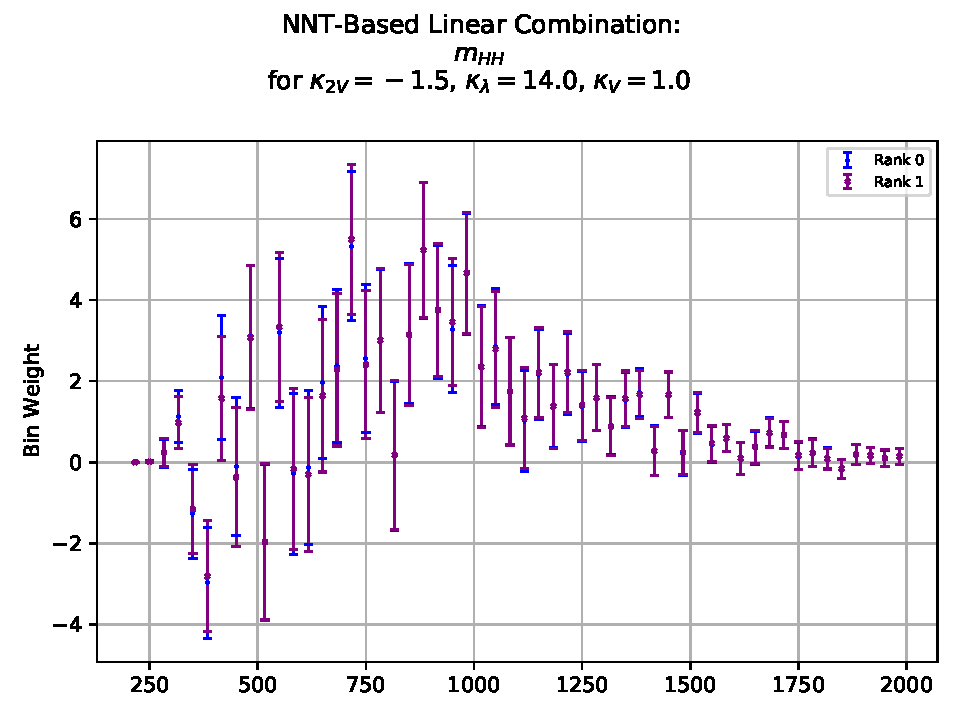
\includegraphics[width=\linewidth,height=\textheight,keepaspectratio]{signal/reco_mHH_compare_preview_auto_top_3D_0-1_cvv-1p5cl14p0cv1p0}
            \captionsetup{justification=centering} \caption{}
        \end{subfigure}
        \begin{subfigure}{0.44\textwidth}
            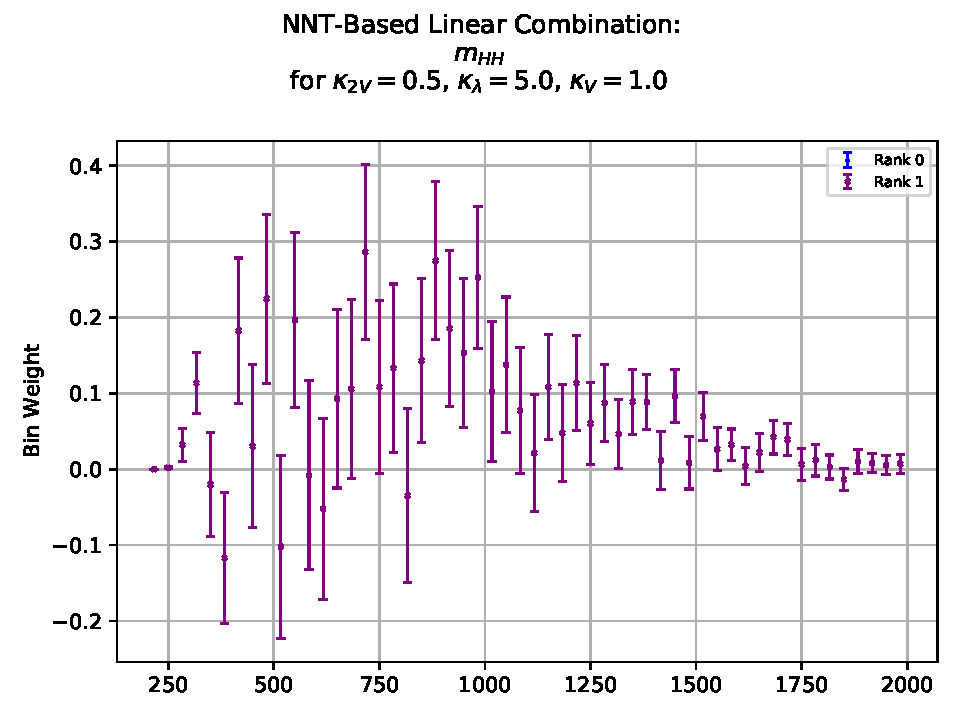
\includegraphics[width=\linewidth,height=\textheight,keepaspectratio]{signal/reco_mHH_compare_preview_auto_top_3D_0-1_cvv0p5cl5p0cv1p0}
            \captionsetup{justification=centering} \caption{}
        \end{subfigure}\\
        \begin{subfigure}{0.44\textwidth}
            \includegraphics[width=\linewidth,height=\textheight,keepaspectratio]{signal/reco_mHH_compare_preview_auto_top_3D_0-1_cvv2p0cl-3p0cv1p0}
            \captionsetup{justification=centering} \caption{}
        \end{subfigure}
        \begin{subfigure}{0.44\textwidth}
            \includegraphics[width=\linewidth,height=\textheight,keepaspectratio]{signal/reco_mHH_compare_preview_auto_top_3D_0-1_cvv2p0cl-9p0cv1p0}
            \captionsetup{justification=centering} \caption{}
        \end{subfigure}
        \caption{
            The two best performing bases of the original 12 MC samples,
                modeling \mhh distributions for points far from the SM.
            Both bases produce very unstable distributions.
        }
        \label{fig:mcpreviews_old}
    \end{figure}


    The proposed solution was to generate one additional MC sample,
        which could be used in combination with five of the original samples to produce a stable basis.
    Of course, until the sample was produced, the negative weight optimization technique could not be used to assess the new sample's performance.
    As such, I developed a novel optimization metric which could predict the performance of a particular basis,
        without the need for any MC production.
    My hypothesis for the behavior of the sample combinations is that the regions of the scale factor space which perform poorly
        (e.g.\ the top left corners of Fig. \ref{fig:mcnWeight_old}),
        do so because one or two of the samples is disproportionately represented in the combination compared to the others.
    The formula for the combination of the samples (c.f.\ Eqn. \ref{eq:combination_general}) amounts to
        weighting each sample's differential cross-section $\xsec_i$ by a $\kappa$-factor-dependent coefficient $g_i(\kvv,\kl,\kv)$,
        and then adding these weighted cross-sections together to obtain the combined differential cross-section.
    Different samples can have cross-sections which are orders of magnitude apart from each other
        (e.g.\ the 1.18 fb cross-section of the SM point VS the 67 fb cross-section of the \kl=10 sample).
    As well, the $\kappa$-factor-based coefficients $g_i$ can vary dramatically across the $\kappa$ space.
    The product of the sample cross-section and the scale factor coefficient (the \textit{weighted cross-section})
        can therefore fluctuate a great deal across the scale factor space.
    For many regions of the $\kappa$ space, it can happen that one or two of the samples' weighted cross-sections vastly outweigh the others.
    In such cases, the combined cross-section is then based almost entirely on these one or two over-represented samples,
        making the combination much more susceptible to statistical deficiencies.
    I propose that this ``closeness'' of the weighted cross-sections can be used as an effective metric of performance
        and one which does not depend on the generation of MC.

    Here I define a metric to quantify this behavior.
    Due to the nature of the weighted cross-sections,
        the metric will be dependent both on the basis samples' cross-section ($\sigma_i$),
        and on the scale factor coefficient ($g_i(\kvv,\kl,\kv)$) of the specific point in the scale factor space to be modeled\footnote{
            Note that I have switched from a binned differential cross-section, to here working with the total cross-section.
            This is possible because the $g_i$ terms are independent of phase-space,
                and therefore do not affect the phase-space integration of the differential cross-section.
        }.
    As well, I want to explicitly note the occurrence of \textit{negative} coefficients in the combination sum.
    My claim is that negative coefficients are \textit{not} intrinsically detrimental to the combination.
    Rather, they merely reflect the behavior inherent to calculating cross-sections,
        in that some Feynman diagrams invariably cancel with others.
    Thus, I will be looking at the ``closeness'' of the \textit{absolute values} of the weighted cross-sections,
        specifically ensuring that bases are \textbf{not} penalized for large cancellations between terms.
    The resulting metric, which I call \textit{Solidarity}, effectively measures how well the basis samples work together at a given point:

    \begin{equation}
        \textrm{\textbf{Solidarity}: }S \equiv \frac{ \sum\limits_{i=1}^6 g_i\sigma_i }{ \textrm{Stdev}(|g_i\sigma_i|) }
        \,.
    \end{equation}

    That is, first take the standard deviation of the absolute values of the $ g_i \sigma_i $ weighted cross-sections.
    Normalize this by the combined cross-section at that point (i.e.\ the sum of the weighted cross-sections).
    Then take the \textit{reciprocal} of this normalized standard deviation,
        such that $S$ increases as the absolute standard deviation gets smaller.
    The advantage of Solidarity as a metric
        is that the cross-section value can be represented by the pure theoretical cross-section.
    So long as the process of reconstruction and selection does not significantly alter the ratios of the various samples' total event yields,
        Solidarity can be used to gauge the performance of a basis without the need for any MC production.

    As the metric is calculated on a per-$\kappa$ basis,
        a heatmap akin to the negative weight heatmap can be generated in a similar manner.

    \begin{figure}[tbh]
    	\centering
        \begin{subfigure}{0.48\textwidth}
            \includegraphics[width=\linewidth,height=\textheight,keepaspectratio]{signal/solidarity_main_rank00old}
            \captionsetup{justification=centering} \caption{}
        \end{subfigure}
        \begin{subfigure}{0.48\textwidth}
            \includegraphics[width=\linewidth,height=\textheight,keepaspectratio]{signal/negative_weights_toprank0}
            \captionsetup{justification=centering} \caption{}
        \end{subfigure}
        \\
        \begin{subfigure}{0.48\textwidth}
            \includegraphics[width=\linewidth,height=\textheight,keepaspectratio]{signal/solidarity_main_rank01}
            \captionsetup{justification=centering} \caption{}
        \end{subfigure}
        \begin{subfigure}{0.5\textwidth}
            \includegraphics[width=\linewidth,height=\textheight,keepaspectratio]{signal/negative_weights_base}
            \captionsetup{justification=centering} \caption{}
        \end{subfigure}
        \caption{
            The heatmap of Solidarity calculated with theoretical cross-section values (left),
                compared to the negative weight heatmap generated by the post-reconstruction and selection MC samples (right).
            The top two plots correspond to the \textit{original} optimal basis (before the inclusion of the 13th sample),
                while the bottom two correspond to the optimal basis sample used in the analysis.
            Note that the regions of low Solidarity values correspond strongly to the regions with large numbers of negative-weighted bins.
            Also note the ``Integral'' values of the different bases (shown just below their titles).
        }
        \label{fig:solidarity_heatmaps}
    \end{figure}

    The map of Solidarity (Fig. \ref{fig:solidarity_heatmaps}) shows a strong relationship with the prevalence of negative-weighted bins,
        despite the Solidarity heatmap being calculated without the use of any MC simulation samples (beyond MadGraph).
    Using the surface integral of the heatmap as was done for the negative-weight map allows a similar metric to be given to a basis as a whole.
    Comparing this theoretical Solidarity integral to the corresponding negative weight integral (Fig. \ref{fig:nWeight_solidarity_scatter})
        shows a very strong correlation between the two,
        which can be exploited to predict useful sample bases before generating any MC samples.

    \begin{figure}[tbh]
        \begin{subfigure}{0.5\textwidth}
            \includegraphics[width=\linewidth,height=\textheight,keepaspectratio]{signal/Nweight_integral_VS_theory_solidarity_integral_old}
            \captionsetup{justification=centering} \caption{Original 12 Samples}
        \end{subfigure}
        \begin{subfigure}{0.5\textwidth}
            \includegraphics[width=\linewidth,height=\textheight,keepaspectratio]{signal/Nweight_integral_VS_theory_solidarity_integral}
            \captionsetup{justification=centering} \caption{Using All 13 Samples}
        \end{subfigure}
        \caption{
            Plots of the negative weight surface integral (calculated from post-reconstruction/selection MC samples)
                of all possible bases, with respect to the same bases' Solidarity surface integral
                (calculated from the theoretical cross-section associated with the MC samples' scale factor values).
            The plot on the left uses only the original 12 available MC samples for its bases.
            To the right is the same plot with the inclusion of the 13th (\kl=-5, \kvv=1, \kv=0.5) sample.
            Note that the plot on the left has a y-axis with a lower bound that is significantly higher ($\sim 250$) 
                than the full-13-sample plot (lower bound $\sim 100$),
                indicating the presence of more optimal bases afforded by the 13th sample.
        }
        \label{fig:nWeight_solidarity_scatter}
    \end{figure}


    Figure \ref{fig:nWeight_solidarity_scatter} was generated using all 1307 linearly independent bases of combining 6 of the 13 available MC samples.
    Due to the strong correlation between negative-weighted bins and solidarity,
        a histogram of only the Theoretical Solidarity surface integral
        (basically just the x-axis of Fig. \ref{fig:nWeight_solidarity_scatter})
        can be used to determine the overall potential performance a set of MC samples might have.
    In order to determine which MC sample should be produced to work most effectively with the already existing 12 samples,
        I constructed such Solidarity surface integral histograms for a wide range of possible new samples.
    Each histogram was constructed using the bases formed from all possible combinations of 6 samples from
        the 12 original samples plus one prospective MC sample.
    Thus, each Solidarity surface integral histogram corresponded to 13 samples,
        and served as a figure of merit for the 13th (the prospective) sample's performance\footnote{
            I would like to note that this brute-force application of Solidarity is far from efficient,
                and any future attempts at producing MC with this metric
                would do well to use a more sophisticated optimization technique.
        }.

    \begin{figure}[tbh]
        \begin{subfigure}{0.5\textwidth}
            \includegraphics[width=\linewidth,height=\textheight,keepaspectratio]{signal/projective_solidarity_all}
            \captionsetup{justification=centering} \caption{All Tested ``13th'' Variation Possibilities}
        \end{subfigure}
        \begin{subfigure}{0.5\textwidth}
            \includegraphics[width=\linewidth,height=\textheight,keepaspectratio]{signal/projective_solidarity_dump}
            \captionsetup{justification=centering} \caption{Close-up of the top of Fig. (a)}
        \end{subfigure}
        \caption{
            A 2D heatmap representation of all the Solidarity integral histograms generated for a myriad of different ``extra sample'' points.
            The rows are sorted from top to bottom by the sum of their bins
                (That is, the sum of all Solidarity surface integrals for all bases associated with the same additional MC sample point).
        }
        \label{fig:solidarity_dump}
    \end{figure}

    Aligning all of these histograms together as in Fig. \ref{fig:solidarity_dump}
        produces a clear method of distinguishing samples that 
        could produce high stability combinations with the existing 12 samples.
    The aggregate sum of all Solidarity surface integrals associated with a new sample
        can evidently be used as a scalar metric by which to rank different prospective scale factor points.
    The culmination of these tests is Fig. \ref{fig:solidarity_performance_map}.

    \begin{figure}[tbh]
        \begin{subfigure}{0.5\textwidth}
            \includegraphics[width=\linewidth,height=\textheight,keepaspectratio]{signal/solidarity_performance_kv1}
            \captionsetup{justification=centering} \caption{\kv = 1}
        \end{subfigure}\\
        \begin{subfigure}{0.5\textwidth}
            \includegraphics[width=\linewidth,height=\textheight,keepaspectratio]{signal/solidarity_performance_kv0p5.pdf}
            \captionsetup{justification=centering} \caption{\kv = 0.5}
        \end{subfigure}
        \begin{subfigure}{0.5\textwidth}
            \includegraphics[width=\linewidth,height=\textheight,keepaspectratio]{signal/solidarity_performance_kv1p5.pdf}
            \captionsetup{justification=centering} \caption{\kv = 1.5}
        \end{subfigure}
        \caption{
            Solidarity cumulative performance maps for various values of \kv.
            The color of a particular (\kvv,\kl) point indicates the overall
                benefit to adding an MC sample with that set of scale factors
                to the existing set of 12 MC samples.
            Colors closer to yellow (the upper end of the scale) denote samples that would improve combination performance,
                while colors closer to purple (the lower end of the scale) denote samples that would be of little to no use if added.
        }
        \label{fig:solidarity_performance_map}
    \end{figure}

    Using Fig. \ref{fig:solidarity_performance_map} as a guide,
        a number of points (mostly those corresponding to the highest aggregate performance values, $\approx 5.5$)
        were selected for limited simulation at truth level.
    Based on the preliminary stability shown by these truth level simulations,
        a full MC production run was generated with its scale factor values set to \kvv=1, \kl=-5, \kv=0.5.
    This set of MC samples combined with the collected data and background estimation,
        can then be used together to test the validity of different possible hypotheses.

\FloatBarrier
\section{Parton Showering Uncertainty}

    Before moving onto the final results, I need to briefly address a small systematic uncertainty associated with the signal MC modelling,
        stemming from the parton showering step of simulation discussed in Section \ref{sec:pythia}.
    To account for differences in different simulation frameworks, an entirely different framework,
        Herwig 7\cite{Bellm:2015jjp}. 
    Herwig performs the same function as Pythia8, but using a different technical implementation.
    The two are fairly consistent in the output kinematics they produce for the \vbfhhproc,
        but there are slight differences (Fig. \ref{fig:pyth_herwig_mjj}).
    A systematic uncertainty is associated with this difference through the following procedure.
    First, a set of MC samples is produced through the same procedure as described in Section \ref{sec:mcsim},
        but using Herwig instead of Pythia8.
    Distributions of \mhh are formed for both of these post-selection MC samples,
        and a bin-by-bin difference calculated in their yields.
    This difference, normalized to the per-bin statistical error, then constitutes the systematic error.
    Now equipped with a model for the background, a model for the signal
        (for any variation of the $\kappa$-values),
        and a suitable accounting of the uncertainties associated with each,
        I can at last proceed to looking at the data and results of the analysis.

    \begin{figure}[tbh] \centering
        \includegraphics[page=64,width=\linewidth,height=0.4\textheight,keepaspectratio]{signal/V2_vbf-hh-4b_l1cvv1cv1}
        \caption{
            VBF jet invariant mass (in GeV) distribution as produced by Pythia8 and Herwig at \textit{truth-level}.
            Pythia8 is displayed in red and Herwig in blue, with their (dominating) region of overlap shown in purple.
            The differences in their behaviour are not dramatic, but are present
                (hence the relatively small associated uncertainty).
        }
        \label{fig:pyth_herwig_mjj}
    \end{figure}

    \begin{figure}
        \centering
        \begin{subfigure}{0.48\textwidth} 
            \includegraphics[width=\linewidth,height=\textheight,keepaspectratio]{signal/VBF_PS_dEta_1_20-1_kl1_k2v1}
            \caption{$\eta < 1.5$ Category}
        \end{subfigure}
        \begin{subfigure}{0.48\textwidth}
            \includegraphics[width=\linewidth,height=\textheight,keepaspectratio]{signal/VBF_PS_dEta_2_20-1_kl1_k2v1}
            \caption{$\eta \geq 1.5$ Category}
        \end{subfigure}
        \caption{
            Systematic uncertainty of the parton showering step of the signal MC generation.
            The ``Nominal'' Parton Showering (PS) MC sample is that derived from Pythia8,
                while the ``Alternate'' (Alt.) sample corresponds to Herwig.
        }
        \label{fig:sig_syst}
    \end{figure}

    


%\section{I'll figure this out later I just wanna jot this down for myself first}

    Here's my more formal attempt at writing down what I do in the 2/3D interpolation

    Overall goal is to measure cross-section of an interaction: ``$\Xsec$".

    Cross-section cannot be measured directly. Instead, we must measure the total number of events ``$T$". 

    The total number of events can be related to the cross-section via the integrated luminosity $L$, by the simple relation $T = \Xsec \times L$.

    This calculation assumes that we can measure all particles across all phase space (emitted at all angles). In practice though, this is not the case.
    Many events are very forward and are never detected by the detector elements.
    Furthermore, due to the need to subtract out background events, many kinematic cuts must be placed on events, further reducing the phase space actually available.
    It is useful then to instead look at the number of events with particles existing in a particular region of phase $\mathscr{E} (q) \equiv \xsec (q) \times L$, where ``$\xsec$" is the differential cross-section.

    The total cross-section is related to the differential cross-section by the relation \\
    $\xsec (q) = d \Xsec / d q$, which can be rearanged for cross-section by integrating over phase space $q$: \\
    $\Xsec = \int \xsec (q) d q$.

    Relating this back to the event counts, we have\\
    $\frac{1}{L} T = \int \frac{1}{L} \mathscr{E} (q) dq $ \\
    $T = \int \mathscr{E} (q) dq $.

    In order to bring this in line with the fact that we cannot simulate an infinite number of events, let's decompose the integral into an infinite sum:\\
    $T = \lim\limits_{N\to\infty} \sum\limits_{n=0}^{N} \mathscr{E}(q_n) dq = \lim\limits_{N\to\infty} \sum\limits_{n=0}^{N} \mathscr{E}(q_n) \Delta q / N $.

    This total is equivalent to the theoretical value only if the number of events is infinite (and thus able to represent all of phase space).
    With a finite number of events, the theoretical total is reduced to an approximation $\tau$, where\\
    $\tau = \sum\limits_{n=0}^{N} \mathscr{E}(q_n) \Delta q / N $.

    The relative space any one event takes in phase space is accounted for in monte-carlo by giving events weights, so this can be rewritten as\\
    $\tau = \sum\limits_{n=0}^{N} w(q_n) = \sum\limits_{n=0}^{N} w_n \quad,\quad w(q_n) \equiv \mathscr{E}(q_n) \Delta q / N $.

    Final analysis of events does not count all events, but rather looks at the distribution of event counts as a function of some specific element of phase space.
    In this analysis, that element is the di-Higgs invariant mass \mhh, and so the event count per bin $m$ in \mhh can be written as\\
    $\tau_m = \sum\limits_{n=0}^{N} w_{nm} $. 

    The effects of performing reconstruction and selection can be represented by a multiplicative factor ``$z(q)$" corresponding to the probability an event with phase-space parameters $q$ will survive selection.
    What remains is the reconstructed event yield\\
    $U(q) = \int z(q) \mathscr{E}(q) dq $.

    Which can be returned to the discrete, finite-event case as\\
    $\mu = \sum\limits_{n=0}^{N} z_n * w_{nm} $.

    Note that in the infinite, continuous case, $z(q)$ is purely binary (in continuous phase-space an event either passes selection or not),
        but becomes a probability $z_n$ when regions of phase-space are aggregated together into the same bin.


\section{Sample Interpolation}

    Simulating, reconstructing, and performing selection on stuff is hard.
    We need to check all points in $\kappa$ space though.
    To address this we can exploit the underlying field-theory mechanics to reverse-engineer a general equation for the number of events expected for any value of the $\kappa$ couplings.
    First, the influence of the couplings can be related to the cross-section through the interaction amplitude ``$\amp$", where\\
    $\amp(q,\kvv,\kl,\kv) =  \kv \kl \matel_s(q) + \kv^2 \matel_t(q) + \kvv \matel_X(q) $

    The differential cross-section is just the absolute square of the amplitude,\\
    \begin{equation}\begin{split}
        \xsec(q,\kvv,\kl,\kv) = |\amp(q,\kvv,\kl,\kv)|^2 &= 
          \kv^2 \kl^2 \matel_s^2(q) + \kv^4 \matel_t^2(q) + \kvv^2 \matel_X^2(q) \\
        &+ \kv^3 \kl (\matel_s^*(q) \matel_t(q) + \matel_t^*(q) \matel_s(q)) \\
        &+ \kv \kl \kvv (\matel_s^*(q) \matel_X(q) + \matel_X^*(q) \matel_s(q) ) \\
        &+ \kv^2 \kvv (\matel_t^*(q) \matel_X(q) + \matel_X^*(q) \matel_t(q) )
    \end{split} \end{equation}

    And the abundance of matrix element cross terms can be absorbed into simple coefficients $a_i(q)$\\
    $\xsec(q,\kvv,\kl,\kv) = \kv^2 \kl^2 a_1(q) + \kv^4 a_2(q) + \kvv^2 a_3(q) + \kv^3 \kl a_4(q) + \kv \kl \kvv a_5(q) + \kv^2 \kvv a_6(q) $


    This can be further simplified by using just $\kappa$ as shorthand for all the couplings,
    so  $\xsec(q,\kvv,\kl,\kv) \to  \xsec(q,\kappa) $, and by collecting the various couplings into a vector\\
    $ \vec{f}(\kappa) = \begin{pmatrix} \kv^2 \kl^2 \\ \kv^4 \\ \kvv^2 \\ \kv^3 \kl \\ \kv \kl \kvv \\ \kv^2 \kvv \end{pmatrix} $

    So we now have\\
    $\xsec(q,\kappa) = f_1(\kappa) a_1(q) + f_2(\kappa) a_2(q) + f_3(\kappa) a_3(q) + f_4(\kappa) a_4(q) + f_5(\kappa) a_5(q) + f_6(\kappa) a_6(q) $

    Which can be written as:  
    $\xsec(q,\kappa) = \vec{a}(q) \bullet \vec{f}(\kappa) $.

    or, adopting Einstein notation, as
    $\xsec(q,\kappa) = a_i(q) f_i(\kappa) $.

    From here we can write this in terms of observed events\\ 
    $T(\kappa) = \int \xsec(q,\kappa) dq \times L = \int a_i(q) f_i(\kappa) dq \times L $.

    And in terms of post-selection events as\\
    $U(\kappa) = \int z(q) \xsec(q,\kappa) dq \times L = \int z(q) a_i(q) f_i(\kappa) dq \times L $.

    To get the number of expected events for any values of the couplings, we only need to find the reconstructed forms of $a(q)_{i}$.
    By running simulations for 6 different, linearly independent variations of $\xsec$, we can obtain the six equations needed to solve for six variables:\\
    $\xsec(q, \kappa_j) = a(q)_{i} f_i(\kappa_j) $, for $j \in {1-6}$. \\
    $\xsec(q, \kappa_j) \to  \xsec_j(q) $, $f_i(\kappa_j) \to F_{ij} $, \\
    $\xsec_{j}(q) = a(q)_{i} F_{ij}$

    Solving for $a$ is just a matter of inverting the matrix $F_{ij}$ \\
    $\xsec_{j}(q) \times F_{ij}^{-1}= a(q)_{i} F_{ij} \times F_{ij}^{-1}$ \\
    $a_{i}(q) = \xsec_{j}(q) F_{ij}^{-1}$ \\
    $a_{i}(q) = \xsec_{j}(q) G_{ji}$, with $G_{ji} \equiv F_{ij}^{-1}$ \\

    With the primed ``$\xsec'$" now denoting a linearly combined cross-section,
        the cross-section for an arbitrary value of the couplings can then be written as
    \begin{equation} \begin{split}
        \xsec'(q, \kappa) &= a_i(q) f_i(\kappa) \\
        \xsec'(q, \kappa) &= \xsec_{j}(q) G_{ji} f_i(\kappa) \\
        \xsec'(q, \kappa) &=  G_{ji} f_i(\kappa) \xsec_{j}(q) \\
        \xsec'(q, \kappa) &=  g_j(\kappa) \xsec_{j}(q) \quad, g_j(\kappa) \equiv G_{ji} f_i(\kappa)
    \end{split} \end{equation}

    Rewriting this in terms of events:
    \begin{equation} \begin{split}
        T'(\kappa) &= \int \xsec'(q,\kappa) dq \times L \\
        T'(\kappa) &= \boxed{\int g_j(\kappa) \xsec_{j}(q) dq \times L = g_j(\kappa) \int \xsec_{j}(q) dq \times L} \\
        T'(\kappa) &= g_j(\kappa) \Xsec_j \times L = g_j(\kappa) T_j \\
        T'(\kappa) &= g_j(\kappa) T_j
    \end{split} \end{equation}

    Note: the boxed section is the key to why this whole combination system works at the event-level as we use it.
    The core reason this can be done is that the $g_j(\kappa)$ coefficient
        \textit{is independant of phase space},
        and thus can be pulled out of the phase space integral.


    This can be repeated for post-selection phase-space:
    \begin{equation} \begin{split}
        U'(\kappa) &= \int z(q) \xsec'(q,\kappa) dq \times L = \int z(q) g_j(\kappa) \xsec_{j}(q) dq \times L \\
        U'(\kappa) &= g_j(\kappa) \int z(q) \xsec_{j}(q) dq \times L = g_j(\kappa) U_j
    \end{split} \end{equation}

    And performed approximately for the discrete, finite case:
    \begin{equation} \begin{split}
        U'(\kappa) &= g_j(\kappa) \int z(q) \xsec_{j}(q) dq \times L \\
        U'(\kappa) &= g_j(\kappa) \lim\limits_{N\to\infty} \sum\limits_{n=0}^{N} z(q) \xsec_{j}(q) dq \times L \\
        U'(\kappa) &= g_j(\kappa) \lim\limits_{N\to\infty} \sum\limits_{n=0}^{N} z(q_n) \xsec_{j}(q_n) \Delta q_n / N \times L \\
        U'(\kappa) \approx \mu' &= g_j(\kappa) \sum\limits_{n=0}^{N} z_n \xsec_{j,n} \Delta q_n / N \times L \\
        \mu' &= g_j(\kappa) \sum\limits_{n=0}^{N} z_n w_{j,n} \times L \\
        \mu' &= g_j(\kappa) \mu_j
    \end{split} \end{equation}



    %Since an observed event count is a collection of many individual events, this can be re-written in terms of individual event weights:\\
    %$T_m(\kappa) = G_{ji} f_i(\kappa) T_{mj}$,\\
    %$T_m(\kappa) = G_{ji} f_i(\kappa) z_{mj} \sum\limits_{n=0}^{N} w_{nmj} $. FIXME I'm not so sure about this way of describing reco-level events










% Ch10: Results - DRAFT 1
% Need to discuss how we put data, the background estimate, and the signal model together
%     and make a claim as to the compatibility of the hypothesis with the data.
% Largely, this means I need to finally understand how pyhf actually works and what the hell the limit framework is doing.
\chapter{Results} \label{chapter:results}

%
%
%
%    I'm not sure I actually have to explain Baye's theorem here...
%    it doesn't appear to be obviously used, or if it is, we're implicitly using the "Uniform" Prior
%    Ask Steve
%
%    L gives probability of seeing the data we have, based on the given model.
%    We need the probability that the given model is the one responsible for the data we see.
%    i.e. we have P(data|model), but we need P(model|data)
%
%    To do this, we need Baye's rule, which comes from the basic 'anding' of probabilities:
%    P(a \& b) = P(a)*P(b|a) , or P(a \& b) = P(b)*P(a|b) . Thus
%    P(a)*P(b|a) = P(b)*P(a|b) 
%    P(b|a) = P(a|b) P(b) / P(a)
%    So we need P(model|data) = P(data|model) * P(model) / P(data)
%
%    For our data we have to use the extended L, which accounts for poisson stats.
%    Basic test is to test mu*S+B for what value of mu is compatible with data
%
%        
%
%
%Statistics is a powerful tool in science,
%    but one which can be very misleading if not used carefully.
%%The oft-used quote comparing lies and statistics exists for a reason;
%%    both can lead to incorrect scientific conclusions.
%%But whereas a lie can be caught by a simple slip of the tongue,
%%    it can take scientists years to discover a slight (intentional or not) mishandling of statistics.
%Unfortunately, the use of statistical methods is not optional.

%To begin, let me propose a much simpler experiment than the one described in this analysis.
%I have a coin, which I suspect may be biased to one side.
%How can I test this?
%A fair coin has a 50/50 chance of landing on either side.
%This means that, were I to flip the coin a large number of times,
%    I would expect a roughly equal number of heads and tails.
%Significant deviation from this ratio (e.g.\ 3 million heads to 1 million tails)
%    would indicate an obvious bias in the coin.
%The conclusion becomes far less obvious however, if the coin is flipped only a few times.
%Even if every flip comes up as heads, no meaningful conclusion can be made if the coin was only flipped e.g.\ four times.
%The crucial questions raised here, which statistical methods are able to address,
%    are how much data is needed to make a decisive statement about a hypothesis,
%    and what kind of statements can be made in lieu of that data.

%The first step to testing a hypothesis,
%    is to know precisely how \textit{likely} any particular outcome is based on that hypothesis.
%The hypothesis for the coin flip is that the probability $p$ of any given flip being heads is 50\%.
%For an experiment consisting of a number of flips $N$,
%    the overall probability of seeing an amount of heads $n$ is given by the binomial distribution:
%\begin{equation}
%    P(n|p) = \tinymatrix{N\\n} p^n (1-p)^{N-n}
%\end{equation}
%Where $P(n|p)$ is read as ``the probability of seeing $n$ heads \textit{given} their probability $p$.''
%With this, 
%
%basic binomial distribution (coin flip) allows obvious p-test. 
%Using a concrete toy example with numbers,
%Show a binomial PDF distro for N flips, and where on that distro the "data" lies
%Show a C-PDF, and again where the data is,
%    and explain that the "unlikeliness" can be used as a test metric, called a "p-value"
%Show of whether or not theory is compatible with data.


% NOTE: From here on, try to keep the p-value concept,
%   as well as the PDF and C-PDF, as a central focus.
% It's easy to conceptualize what a p-value is,
% so you should keep returning to it in order to retain 
% a concrete basis for all the weird math you're about to do
\section{Statistical Mathematics}

    I have thus far established how the analysis has collected its data,
        how it has estimated the amount of background present in that data,
        and how it has modeled the hypothesis for the HH process to be tested with that data.
    With these assembled, the final step is to arrange them together in order to make a definitive statement
        as to the validity or incompatibility of the hypothesis with the provided data.
    More plainly, the questions for this chapter are:
        was the di-Higgs process detected in the data,
        and what were the values of the $\kappa$ scale factors involved in its production?
    To answer these questions, I must turn to the field of statistical analysis.
    In this chapter, I want to explain why statistics is required for this analysis,
        discuss the specific statistical techniques this analysis uses,
        and conclude with what those techniques reveal in light of the data presented.

    % Introduce poisson statistics with single counting variable and only signal w/ toy example.
    % Discuss difference between coin toss and radioactivity.
    % i.e. that with a coin toss, the number to tosses is entirely determined by me, and is thus fixed.
    % For decay and such, the number of events is completely random, and what is fixed is how much time (luminosity)
    %     the experiment is given.
    Like most particle physics processes, the $VBF \to HH \to 4b$ process results in a need to count outcomes,
        a fundamentally Poissonian situation.
    The number $n$ of di-Higgs process that are observed in ATLAS can then be modeled with a Poisson distribution\cite{cranmer2015practical}:
    \begin{equation}
        P(n|\nu) = \frac{ \nu^n e^{-\nu} }{n!}
    \end{equation}
    This function $P(n|\nu)$ can be read as ``the probability $P$ of obtaining $n$ events \textit{given} the parameter $\nu$.''
    That is, for a process which is expected on average to produce $\nu$ number of events,
        this function gives the probability that such a process would produce $n$ events.

    The compatibility of a hypothesis with data can be established by use of a ``p-value test.''
    As an example, take the case of a simple alpha particle emitter with an unknown emission rate
        which I hypothesize emits radiation at a rate of once per minute.
    After one hour, I would expect on average 60 events.
    Running the experiment, I find that 68 events were detected.
    Plotting the Poisson distribution for $P(n|60)$ (Fig. \ref{fig:poisson_toy_sig:pdf}),
        I can see how likely an observation of 68 events is.
    \begin{figure}
        \centering
        \begin{subfigure}{0.48\textwidth} 
            \includegraphics[width=\linewidth,height=\textheight,keepaspectratio]{results/toy_poisson}
            \caption{Toy Poisson PDF}
            \label{fig:poisson_toy_sig:pdf}
        \end{subfigure}
        \begin{subfigure}{0.48\textwidth}
            \includegraphics[width=\linewidth,height=\textheight,keepaspectratio]{results/toy_Cpoisson}
            \caption{Toy Poisson Cumulative PDF}
            \label{fig:poisson_toy_sig:Cpdf}
        \end{subfigure}
        \caption{
            A plot of the probability distribution function (PDF)
                and cumulative PDF for a toy Poisson experiment.
        }
    \end{figure}

    \FloatBarrier
    A ``p-test'' is the key tool that will be used throughout the rest of the analysis.
    Its goal is to find the probability that, were my hypothesis correct,
        I would obtain data with a value \textit{at least as extreme} as what I measured\footnote{
            There are actually several different variations of a p-test;
            this is specifically a one-sided p-test}.
    So the p-value for an event rate of 68, given an expected average of 60, can be found by taking:
    \begin{equation}
        \textrm{p-value}(n=68) = P(68|60) + P(69|60) + P(70|60) ... P(\infty|60) = \sum\limits_{m=n}^\infty P(m|60)
    \end{equation}
    This is best visualized using the \textit{cumulative} probability distribution function (Fig. \ref{fig:poisson_toy_sig:Cpdf}).
    In this example, the p-value would be 0.17.
    A typical standard for many statistical tests, and the one used in this analysis,
        is to establish a ``Confidence Level'' (CL) in the results of an experiment at a level of 95\%. 
    The confidence level is simply $1-p$, so a CL of 0.95 corresponds to a p-value of less than 0.05.
    Because this toy experiment has a p-value larger than 0.05,
        the conclusion would be that ``the hypothesis was compatible with the data within a CL of 95\%.''


    % Introduce background
    % Ditch toy, pull out actual Background and Signal (SM) event yields.
    % Should also probably dig up the "sensitivity" metric and show how bad that is here as well.
    % CLs = CLs+b/CLb explained in (Barlow:2019svl pg. 192)
    % The abysmal performance here should justify splitting the event into bins,
    %     in order to identify regions of Mhh that we are more sensitive to.
    % Using multiple bins however, dramatically complicates the statistical analysis.
    % Enter the profile likelihood fit.
    Moving on from the toy example, the hypothesis being tested in this analysis
        involves a background event rate in addition to the signal hypothesis being considered.
    The average number of events expected is then $\nu = S + B$,
        where $S$ and $B$ are the signal and background rate yields respectively.
    The confidence limits in such a situation are handled in different ways from one analysis to another,
        but in this analysis the p-value of the signal alone is given by
    \begin{equation}
        P_S = \frac{P_{S+B}}{1 - P_B}
    \end{equation}
    % TODO: for example, in the case where the oberved number of events is far larger than the background estimate,
    %   such that the background is entirely unable to account for the observation,
    %   P_B will be approximately 1, and 1-P_B will approach 0.
    %   This will in turn scale P_{S+B} up dramatically,
    %   emphasizing that since the background is unable to describe the observation,
    %   the signal must be present to account for the difference.
    Where $P_{S+B}$ is the p-value of the hypothesis assuming the signal is present,
        and $P_B$ is the p-value of the background-only hypothesis
        (often called the ``null hypothesis,'' $H_0$)\cite{Barlow:2019svl}.
    The total yields of the data, Background estimate, and SM signal hypothesis are provided in Table \ref{tab:event_yield},
        and their PDF and cumulative PDF can be seen in
        Fig. \ref{fig:poisson_sig:pdf} and \ref{fig:poisson_sig:Cpdf}.

    \begin{table}[tbh]
       \begin{center}
           \caption{Estimated and Observed Event Yields}
           \label{tab:event_yield}
           \footnotesize
           \begin{tabular}{|l|l|}
           \toprule
               Type  &	Event Yield \\
               \midrule
               Signal Hypothesis (SM) & 0.36 \\
               Signal Hypothesis (\kvv=3) & 52.7 \\
               Background Estimate  & 493.6 \\
               Observed Data & 495 \\
           \bottomrule
           \end{tabular}
       \end{center}
    \end{table}

    \begin{figure}
        \centering
        \begin{subfigure}{0.48\textwidth} 
            \includegraphics[width=\linewidth,height=\textheight,keepaspectratio]{results/total_yield_poisson}
            \caption{Poisson PDF}
            \label{fig:poisson_sig:pdf}
        \end{subfigure}
        \begin{subfigure}{0.48\textwidth}
            \includegraphics[width=\linewidth,height=\textheight,keepaspectratio]{results/total_yield_Cpoisson}
            \caption{Poisson Cumulative PDF}
            \label{fig:poisson_sig:Cpdf}
        \end{subfigure}
        \caption{
            A plot of the probability distribution function (PDF)
                and cumulative PDF for the estimated background and simulated signal,
                with the observed yield denoted in both.
        }
    \end{figure}

    The p-value of the signal based on the observed yield is 0.46,
        for a CL of 54\%.
    This indicates that the signal is very compatible with the data,
        but by no means indicates proof for the di-Higgs process.
    To understand why, one need only look at the CL on the background-only hypothesis.
    Proof of the di-Higgs process would necessitate an excess of events so significant that
        the null hypothesis must be rejected (typically $P_B < 10^{-7}$, the ``$5\sigma$'' discovery limit).
    Here though, $P_B = 0.31$, which means the null hypothesis is \textit{also} highly compatible with the data,
        and cannot be rejected.

    \begin{figure}
        \centering
        \begin{subfigure}{0.48\textwidth} 
            \includegraphics[width=\linewidth,height=\textheight,keepaspectratio]{results/mhh_yield_SM}
            \caption{Event yields with SM Signal [TODO: make this plot better with labels and stuff]}
            \label{fig:mhh_yield:kvv1}
        \end{subfigure}
        \begin{subfigure}{0.48\textwidth}
            \includegraphics[width=\linewidth,height=\textheight,keepaspectratio]{results/mhh_yield_SM}
            \caption{Event yields with Signal \kvv=3 [TODO: actually grab the kvv=3 distro]}
            \label{fig:mhh_yield:kvv3}
        \end{subfigure}
        \caption{
            The event yields of the data, background, and signal binned by their \mhh distribution.
            The bottom plot displays the ``sensitivity'' ($Z_s=\frac{S}{\sqrt{S+B}}$)
                of the analysis to a particular \mhh bin.
            A sensitivity value of $\approx 2$ is usually necessary to achieve a CL around 95\%.
            [Hey Steve do I need to explain sensitivity in detail? Also do I have this right?]
        }
    \end{figure}


    The issue of course, is that the signal is utterly dwarfed by the quantity of background events.
    A method of circumventing this scale issue
        is to break the event count up across a number of different
        bins and categories dependent on kinematic observables of the events.
    The signal and background events are expected to have their events distributed differently across such observables.
    Thus, even though there are vastly more background events overall,
        it is entirely possible for there to exist a region in the observable space
        in which there are a comparable number of signal events.
    In this analysis, the primary observable variable is the di-Higgs invariant mass, \mhh.
    Ultimately, the final test of the hypothesis will still be to create a cumulative PDF distribution,
        obtain the p-value of the cumulative PDF for the observed data, and use that to derive a CL for the signal.
    With multiple bins (as well as categories and uncertainties) however,
        the derivation of the cumulative PDF becomes much more complex.
    The following section will describe precisely how all these aspects of the analysis are combined together,
        producing a much more powerful statistical analysis.


\FloatBarrier
% Discuss sources of error, assumptions, categorization, concept of mu values;
% basically all the complicated stuff the limit framework is doing
% Make the final goal to be establishing a p-value via the cumulative PDF distro,
%   as was done for the simple coin toss example (to bring things full circle)
\section{VBF HH 4b Limit-Setting Framework}
    
    %What is a test statistic and why do we need it?
    The statistical technique used here to obtain a cumulative PDF
        is based on the use of a ``test statistic'' derived through a \textit{profile likelihood fit}.
    Test statistics come in many forms, but the one used here is the \qtil test statistic.
    \qtil is technically defined in a single equation,
        but that equation involves so many parameters that it is worth breaking it down into steps.

    % Introduce mu*S+B format.
    % Discuss formula for L specifically in this analysis
    %    (emphasis on explaining the bits in parentheses):

    %    L = product[ for each category (2: eta hi and lo) 
    %        product[for each bin: poissons]
    %        * product[ nuissance params (4 for bgd shape error, 1 for norm error) ] 
    %    ]
    %    
    The first step to deriving \qtil is to slightly redefine the expectation value for the number of events 
        with a scaling factor $\mu$ applied to the signal yield.
    $\mu$ is referred to as the ``Parameter of Interest'' (PoI),
        and allows the yield of the signal process to be adjusted to some ideal value that best fits the data.
    As well, since there are now multiple bins $i$ (each with their own expectation values)
        the new definition of the expectation value is
    \begin{equation}
        \nu_i(\mu) = \mu S_i + B_i
    \end{equation}
    Instead of a probability distribution function, now a ``likelihood'' function $L$ will be used,
        which is the joint probability of the observed data $n$ in each of the bins
        (which are in turn all Poisson distributed with expectation value $\nu_i$)
    \begin{equation}
        L(n,\mu) = \prod \limits_{i=1}^{N} P(n_i | \nu_i)
            = \prod \limits_{i=1}^{N} \frac{ (\mu S_i + B_i)^{n_i} e^{\mu S_i + B_i} }{n_i!}
    \end{equation}
    Where $i$ runs over all the $N$ bins.
    Note that unlike a PDF, the sum of all outcomes from the likelihood function will \textit{not} sum to unity,
        and so the likelihood function does not constitute a probability distribution function\cite{cousins2020likelihood}.

    % Discuss uncertainties and categories
    Uncertainties present in the background estimate add another layer of complexity to the likelihood function,
        because uncertain parameters must be fit as well as the parameter of interest.
    The expectation value is further adjusted to be $\nu_i(\mu, \Theta) = \mu S + \Theta B$,
        where $\Theta$ is a product of five scaling values 
    \begin{equation}
        \Theta = \prod \limits_{a=0}^{4}  \theta^a
    \end{equation}
    These scaling values, called ``nuisance parameters,''
        correspond to the four shape uncertainties $\sigma_i^a, a\in{1,2,3,4}$
        and one normalization uncertainty $\sigma^0$ ($\sigma^0$ does not vary by bin),
        which were described in Section \ref{sec:nn_training}
        [TODO: you need to go back and describe these uncertainties better now that you understand them].
    Here the background uncertainty is modeled as a Gaussian with expectation value $\theta^a B_i$ and standard deviation $\sigma_i^a$.
    Extending the likelihood function with the nuisance parameters produces
    \begin{equation} \begin{split}
        L(n,\mu,\Theta) &= \prod \limits_{i=1}^{N} P_{\textrm{poiss}}(n_i | \nu_i) 
             \prod \limits_{a=0}^{4} P_{\textrm{gauss}}(n_i | \nu_i, \sigma_i^a) 
        \\&= \prod \limits_{i=1}^{N} \frac{ (\mu S_i + \Theta B_i)^{n_i} e^{\mu S_i + \Theta B_i} }{n_i!} \times
            \prod \limits_{a=0}^4 \frac{1}{\sigma_i^a \sqrt{2\pi}} e^{
                -\frac{1}{2}\left(\frac{n_i- (\mu S_i + \Theta B_i)}{\sigma_i^a}\right)^2
            }
    \end{split} \end{equation}

    Finally, in order to increase sensitivity further, events are split into two different categories
        based on whether the \deta separation between the reconstructed Higgs Bosons is greater or less than 1.5.
    The full likelihood function is then a product over the two categories
    \begin{equation}
        L(n,\mu,\Theta) = \prod \limits_{j=1}^{2}
             \prod \limits_{i=1}^{N} P_{\textrm{poiss}}(n_{ij} | \nu_{ij}) 
             \prod \limits_{a=0}^{4} P_{\textrm{gauss}}(n_{ij} | \nu_{ij}, \sigma_{i}^a) 
    \end{equation}

    % Discuss nuissance parameter fitting
    There is only one parameter of interest ($\mu$), but there are now six parameters $L$ is a function of.
    To address this without over-fitting to the data, a maximized fit is performed across the nuisance parameters.
    Such a fit eliminates their presence from the likelihood function, but it should be noted that it does so at a cost.
    The nuisance parameter fit significantly extends the final cumulative PDF, reducing the overall confidence intervals.
    To perform this fit, the value of $\mu$ is fixed to the desired scale (for now $\mu=1$),
        and then $L(n,\mu,\Theta)$ is maximized over the various values of the $\theta^a$.
    The nuisance parameter values are then fixed to this maximal value $\hat{\hat\theta}^a$, such that
    \begin{equation}
        \prod \limits_{a=0}^{4} \frac{\partial}{\partial \theta^a} L(n,\mu,\Theta) |_{\Theta=\hat{\hat\Theta}} = 0
    \end{equation}
    Resulting in a fitted $L = L(n,\mu,\hat{\hat\Theta})$.
    [TODO: I still don't know how the stat errors get factored into all this...
        are they treated the same way as the nuissance params,
        or are they somehow intrinsic to the poisson distribution?
    Stat error for poisson is just sqrt(expectation),
        so maybe the stat error is automatic?
    Or is there some deeply unpleasant error propogation going on under the pyhf hood?]
        
    %lambda = L(mu, theta vary-opt) / L(mu-opt, theta-opt);
    As a final fitting step, the likelihood $L$ is normalized to a fully maximized value $\hat L$,
        to create a quantity $\lambda = L / \hat L$.
    $\hat L$ is formed in a similar manner to $L$, but whereas $L$ has a fixed value for $\mu$,
        $\hat L$ allows $\mu$ to also be a free parameter.
    It is then maximized with regard to both $\mu$ and the nuisance parameters such that
    \begin{equation}
        \prod \limits_{a=0}^{4} \frac{\partial}{\partial \theta^a} \frac{\partial}{\partial \mu} L(n,\mu,\Theta) |_{\Theta=\hat \Theta} |_{\mu=\hat \mu} = 0
    \end{equation}
    A test statistic $t$ can now be constructed with $\lambda$, as
    \begin{equation}
        t = -2 \ln{\lambda} = -2 \ln{\frac{L(\mu, \hat {\hat \Theta})}{L(\hat \mu, \hat \Theta)}}
    \end{equation}
    It is worth briefly reviewing what this formula and its pieces mean before moving onto the last step.
    The likelihood $L$ is just the joint probability that every bin of the observed data would have the values they do,
        based on the modeled expectation values.
    Due to the large number of bins, $L$ will always be an extremely small number between 0 and 1.
    By construction, $\hat L$ will always be a joint probability at least as large as $L$, though still between 0 and 1.
    Their ratio $\lambda$ represents how close $L$ is to being maximally likely for the given set of observed data and models.
    $\lambda$ can at most be equal to 1, indicating that $L$ is nearly equal to $\hat L$,
        which in turn indicates that the model fits the observed data as well as it can for any given value of $\mu$.
    In turn, a value near 0 indicates that the observed data is exceedingly unlikely to have come from the model with the given $\mu$,
        compared to the much more likely model based on the optimal value of $\mu$.
    The test statistic $t$ then has a simple interpretation:
        values of $t$ close to 0 indicate high likelihood,
        and the higher the value of $t$ (up to infinity) the more unlikely it is that the model is compatible with the data.

    %q~ = t with edge cases;
    At last, the desired test statistic \qtil can be derived, as a piece-wise variation on $t$\cite{asymptotic_formulae_for_likelihood}:
    \begin{equation}
        \qtil = \begin{cases}
            -2 \ln{\frac{L(\mu, \hat {\hat \Theta})}{L(0, \hat \Theta(\mu=0))}} & \hat \mu < 0,\\
            -2 \ln{\frac{L(\mu, \hat {\hat \Theta})}{L(\hat \mu, \hat \Theta)}} & 0 \leq \hat \mu \leq \mu,\\
            0 & \mu < \hat \mu 
        \end{cases}
    \end{equation}
    The middle condition is simply $t$, with the top and bottom edge cases being the defining traits of \qtil.
    \qtil in particular is used for this analysis because of these piece-wise conditions,
        which enforce the fact that $\mu$ should never be negative (the signal cannot remove events from the background),
        and that this analysis is only interested in establishing a lower-bound
        [TODO: might need to think about this some more to be sure you know what you're saying here].

    %Single mu vs q~ PDF constructed from monte-carlo distros
    %C-PDF showing where mu-model resides for Psb, Pb, and finally Ps=Psb/(1-Pb)
    %In practice, the q~ CPDF distros are estimated using an asymptotic approximation method\cite{asymptotic_formulae_for_likelihood}.
    %(because the MC method is way too slow)
    Even with the test statistic \qtil available, its use may not be immediately obvious.
    Recall that the goal is to produce a cumulative probability distribution function,
        which can be compared against to obtain a p-value.
    In order to obtain a distribution, it must be created using Monte-Carlo techniques.
    A large number of simulated distributions can be generated,
        sampled from the modeled signal and background Poisson distributions.
    For each of these simulated ``observations'' the test statistic \qtil can be derived.
    The result is a collection of \qtil values, which together comprise a distribution.
    A cumulative probability distribution can be constructed with this distribution,
        by simply taking the fraction of simulated observations which fall below some value of the observed \qtil.
    Figures \ref{fig:qtil:pdf} and \ref{fig:qtil:Cpdf} demonstrate how this is done,
        as well as where the SM signal model falls with a $\mu$ value of 1.

    \begin{figure}
        \centering
        \begin{subfigure}{0.48\textwidth} 
            \includegraphics[width=\linewidth,height=\textheight,keepaspectratio]{results/mu_pdf}
            \caption{Values of \qtil for Simulated Distributions}
            \label{fig:qtil:pdf}
        \end{subfigure}
        \begin{subfigure}{0.48\textwidth}
            \includegraphics[width=\linewidth,height=\textheight,keepaspectratio]{results/mu_pdf}
            \caption{Cumulative PDF of \qtil Test Statistic}
            \label{fig:qtil:Cpdf}
        \end{subfigure}
        \caption{
            [TODO: replace the placeholders with the real thing.]
            [Steve, so these will be by far the most involved plots here,
                because I'm trying to generate them by reverse engineering the entire limit framework and pyhf.
            If I can finish them, it's a nice proof to myself that I understand how everything is actually done.
            But I may not have enough time to finish this,
                in which case I'll probably just scrap these figures and the references to them.]
            Plots of the values and cumulative PDF based on \qtil,
                with the \qtil value of the observed data highlighted.
            Note the ``error bands'' which provide extended regions of higher confidence.
            These are produced via the formula [TODO: how do I still not know how these are made?!].
        }
    \end{figure}

    I would like to note that while I have performed the explicit simulation of the MC distributions for the sake of these figures,
        in practice the MC approach is far too slow.
    What is often done instead, and what this analysis in particular does (via the Pyhf python framework),
        is to use an asymptotic approximation to the \qtil cumulative distribution function.
    The derivation of this approximation is well beyond the scope of this thesis,
        but is documented extensively by Cowan\cite{asymptotic_formulae_for_likelihood}.
    \qtil itself still needs to be calculated for the observed data,
        but the asymptotic approximation allows for rapid and accurate calculation of its p-value.
    Now that I finally have a robust mechanism for calculating the p-value of the di-Higgs signal hypothesis,
        the only step remaining is to use it.

\FloatBarrier
% Finally, I need to reveal what our final results actually are, and what they mean.
% This will mostly just be plots of mu values, limit values, and my 2D exclusion plots.
% I can discuss the shapes and stuff here, as well as talk about any mismatches between expected and observed results.
% Be ready to just put in filler results, since we probably won't have unblinded by the time I get here.
\section{Final Interpretation}

    [Hey steve, for this first edit round, don't worry about the formatting of any of the plots in this section.
    They all need to be replaced when we unblind, and we've been updating their format a lot. (these are pretty old)]
    [FIXME: literally all the plots and numbers and conclusions here need to be updated once we unblind]
    All limits quoted in this analysis are to a CL of 95\%.
    The CL of the SM signal hypothesis with a $\mu$ scale of 1,
        even with the extensive profile likelihood fit technique, is still only 50\% [FIME].
    No meaningful conclusion can be drawn from such a small signal.
    However, looking at the \kvv=3 signal model at a $\mu$ scale of 1 provides a CL of $\approx 99\%$,
        which indicates that a value of \kvv=3 is incompatible with data, and so can be excluded.
    This result suggests a much more useful way of performing these tests.
    For each signal hypothesis, a series of increasing values of $\mu$ can be tested against the observed data,
        each with their own CL value.
    A series of such tests can be seen in Fig. \ref{fig:mu_CL_vals}.

    \begin{figure}
        \centering
        \begin{subfigure}{0.48\textwidth} 
            \includegraphics[width=\linewidth,height=\textheight,keepaspectratio]{results/brazilplot_full_3D_scan_NEO2021_samps_vbf_pd_161718_kl_1-00_k2v_0-00_k1v_1-00}
            \caption{Values of \qtil for Simulated Distributions}
            \label{fig:mu_CL_k2v0}
        \end{subfigure}
        \begin{subfigure}{0.48\textwidth} 
            \includegraphics[width=\linewidth,height=\textheight,keepaspectratio]{results/brazilplot_full_3D_scan_NEO2021_samps_vbf_pd_161718_kl_1-00_k2v_1-00_k1v_1-00}
            \caption{Values of \qtil for Simulated Distributions}
            \label{fig:mu_CL_k2v1}
        \end{subfigure} \\
        \begin{subfigure}{0.48\textwidth}
            \includegraphics[width=\linewidth,height=\textheight,keepaspectratio]{results/brazilplot_full_3D_scan_NEO2021_samps_vbf_pd_161718_kl_1-00_k2v_1-50_k1v_1-00}
            \caption{Cumulative PDF of \qtil Test Statistic}
            \label{fig:mu_CL_k2v1.5}
        \end{subfigure}
        \begin{subfigure}{0.48\textwidth}
            \includegraphics[width=\linewidth,height=\textheight,keepaspectratio]{results/brazilplot_full_3D_scan_NEO2021_samps_vbf_pd_161718_kl_1-00_k2v_3-00_k1v_1-00}
            \caption{Cumulative PDF of \qtil Test Statistic}
            \label{fig:mu_CL_k2v3}
        \end{subfigure}
        \caption{
            [Wow the labels on these plots are super wrong. Pretty sure y is supposed to be the p-value,
                and the red line is the 0.05 mark. I think these are fixed in the updated plots?]
        }\label{fig:mu_CL_vals}
    \end{figure}

    \FloatBarrier
    The critical value for each of the plots in Fig. \ref{fig:mu_CL_vals} is the 95\% CL $\mu$.
    A more general plot can be created from this by showing the CL=95\% $\mu$
        exclusion value as a function of the scale factor value $\kvv$.
    Utilizing the signal model linear combination equation from Section \ref{sec:signal_combination},
        the signal hypothesis for any value of \kvv can be tested, producing Fig. \ref{fig:kvv_SM_scan}.

    \begin{figure}
        \includegraphics[width=\linewidth,height=\textheight,keepaspectratio]{results/k2v_scan_full_3D_scan_NEO2021_samps_vbf_pd_161718_kl_1-0_xsec.png}
        \caption{DiHiggs signal \kvv exclusion plot.
            The red line indicates the theoretical cross-section of the di-Higgs interaction as a function of \kvv.
            The dashed line is formed as the product of the theoretical cross-section value
                and the 95\% CL value of $\mu$ for that \kvv signal}
        \label{fig:kvv_SM_scan}
    \end{figure}

    Figure \ref{fig:kvv_SM_scan} is arguably the single most significant result presented in this thesis,
        as it indicates that \kvv=0 can be excluded with a CL of 95\% [To Steve: look I can hope alright].
    This in turn provides strong evidence for the existence of the \HHVV interaction process.
    Yet, there is still more to discuss.

    The signal combination formula is able to produce a signal hypothesis with multiple scale factor values adjusted at once,
        and so a wide range of \kvv scan plots can be produced, as seen in Fig. \ref{fig:kvv_multi_kl}

    \begin{figure}
        \centering
        \begin{subfigure}{0.48\textwidth} 
            \includegraphics[width=\linewidth,height=\textheight,keepaspectratio]{results/k2v_scan_full_3D_scan_NEO2021_samps_vbf_pd_161718_kl_-4-0_xsec.png}
            \caption{\kvv Exclusion, \kl=-4}
            \label{fig:kvv_scan_kl0}
        \end{subfigure}
        \begin{subfigure}{0.48\textwidth} 
            \includegraphics[width=\linewidth,height=\textheight,keepaspectratio]{results/k2v_scan_full_3D_scan_NEO2021_samps_vbf_pd_161718_kl_0-0_xsec.png}
            \caption{\kvv Exclusion, \kl=0}
            \label{fig:kvv_scan_kl1}
        \end{subfigure} \\
        \begin{subfigure}{0.48\textwidth}
            \includegraphics[width=\linewidth,height=\textheight,keepaspectratio]{results/k2v_scan_full_3D_scan_NEO2021_samps_vbf_pd_161718_kl_2-0_xsec.png}
            \caption{\kvv Exclusion, \kl=2}
            \label{fig:kvv_scan_kl2}
        \end{subfigure}
        \begin{subfigure}{0.48\textwidth}
            \includegraphics[width=\linewidth,height=\textheight,keepaspectratio]{results/k2v_scan_full_3D_scan_NEO2021_samps_vbf_pd_161718_kl_10-0_xsec.png}
            \caption{\kvv Exclusion, \kl=10}
            \label{fig:kvv_scan_kl10}
        \end{subfigure}
        \caption{
            A collection of \kvv exclusion scan plots, with the \kl scale factor set to alternate values.
        }\label{fig:kvv_multi_kl}
    \end{figure}

    \FloatBarrier
    This abundance of parameter space can be collapsed by taking special note only of
        the individual points at which the theoretical cross-section and observed 95\% CL cross-section intersect,
        as these points indicate where the regions of exclusion lie (Fig. \ref{fig:kvv_kl_2Dscan}).

    \begin{figure}
        \includegraphics[width=\linewidth,height=\textheight,keepaspectratio]{results/2D_scan_full_3D_scan_NEO2021_samps_vbf_pd_161718_k1v1_exclusion}
        \caption{Two-dimensional \kvv/\kl exclusion plot, for \kv=1.
            Signal hypothesis model corresponding to scale factors that lie
                \textit{outside} the ellipsoidal region are incompatible with the observed data to a CL of 95\%,
                and thus can be excluded.
            }
        \label{fig:kvv_kl_2Dscan}
    \end{figure}

    Finally, by utilizing the full dimensionality afforded by the 6-term signal combination equation,
        such scan plots can be produced across multiple slices of \kv.
    \kv is already highly constrained, and Fig. \ref{fig:kvv_kl_multislice}
        reveals that within the established bounds on \kv,
        the constraints on \kl and \kvv differ by very little.

    \begin{figure}
        \centering
        \begin{subfigure}{0.48\textwidth} 
            \includegraphics[width=\linewidth,height=\textheight,keepaspectratio]{results/2D_scan_full_3D_scan_NEO2021_samps_vbf_pd_161718_k1v0-96_exclusion}
            \caption{\kvv/\kl Exclusion, \kv=0.96}
            \label{fig:kvv_kl_2Dscan_kv0.96}
        \end{subfigure}
        \begin{subfigure}{0.48\textwidth} 
            \includegraphics[width=\linewidth,height=\textheight,keepaspectratio]{results/2D_scan_full_3D_scan_NEO2021_samps_vbf_pd_161718_k1v1_exclusion}
            \caption{\kvv/\kl Exclusion, \kv=1.00}
            \label{fig:kvv_kl_2Dscan_kv1}
        \end{subfigure} \\
        \begin{subfigure}{0.48\textwidth}
            \includegraphics[width=\linewidth,height=\textheight,keepaspectratio]{results/2D_scan_full_3D_scan_NEO2021_samps_vbf_pd_161718_k1v1-03_exclusion}
            \caption{\kvv/\kl Exclusion, \kv=1.03}
            \label{fig:kvv_kl_2Dscan_kv1.03}
        \end{subfigure}
        \begin{subfigure}{0.48\textwidth}
            \includegraphics[width=\linewidth,height=\textheight,keepaspectratio]{results/2D_scan_full_3D_scan_NEO2021_samps_vbf_pd_161718_k1v1-06_exclusion}
            \caption{\kvv/\kl Exclusion, \kv=1.06}
            \label{fig:kvv_kl_2Dscan_kv1.06}
        \end{subfigure}
        \caption{Two-dimensional \kvv/\kl exclusion plot, for multiple values of \kv.
            Recall that \kv has been measured as $1.05 \pm 0.04$,
                hence the heavy restriction in its range here.
            Within this range, the \kvv/\kl limits do deviate slightly from their \kv=1 values,
                but not by a dramatic amount.
        }\label{fig:kvv_kl_multislice}
    \end{figure}


% Ch11: Conclusion and Future Studies - DRAFT 0
\chapter{Conclusion}\label{chapter:conclusion}

%Summarize thesis
This thesis used 126 $\textit{fb}^{-1}$ of data from run 2 of ATLAS
    to perform a search of the \hhproc process decaying to 4 bottom quarks,
    in order to better constrain the \kl and \kvv Higgs self-coupling constants.
The analysis made extensive use of the b-jet trigger system to identify this final state,
    alongside a b-jet pairing algorithm capable of accurately reconstructing the di-Higgs system.
An efficient selection algorithm was also employed to remove a majority of background events,
    though a sizable background still remained.
This fully hadronic final-state background was estimated using a sophisticated data-driven approach,
    which takes advantage of machine-learning algorithms specifically designed around the VBF environment.
The di-Higgs signal itself was then modeled using six Monte-Carlo simulations.
These six models were extended across the entirety of the possible \kvv/\kl/\kvv coupling parameter space
    through a linear combination technique
    which operated by reverse-engineering the fundamental QFT cross-section equation for the HH process.
Although this method initially met with severe instabilities in its modeling performance,
    I was able to derive a novel optimization procedure able to specify
    the exact Monte-Carlo simulation needed to stabilize the combination.
This additional MC sample was then used to provide an accurate hypothesis description across
    the three-dimensional \kvv/\kl/\kv parameter space,
    and so establish exclusion limits across these coupling values. 

%signal
Though the di-Higgs process itself is still too elusive for discovery with the amount of data collected so far,
    significantly tighter constraints can be placed on the \kvv and \kl coupling constants.
Indeed, for the first time constraints have been placed on the full
    3D coupling space observable via the VBF production mode of the di-Higgs process.
Courtesy of the MC sample linear combination technique,
    \kl has been constrained to between -19.5 and 23.0 for all values of \kvv with a fixed \kv=1,
    and between -10.1 and 13.3 for $\kvv=\kv=1$.
Likewise, the extrema of \kvv have been established between -0.8 and 2.8
    if \kl is permitted to fluctuate beyond its SM value while \kv is fixed to 1.
The most noteworthy results of this thesis however, is that for $\kl=\kv=1$,
    the value of \kvv can be excluded to a confidence of 95\% outside the range of $0.1 < \kvv < 2.0$.
This marks the tightest published constraints to date, improving over the latest results from CMS
    of $-0.1 < \kvv < 2.2$\cite{cms_results}.
%This leaves only one of two options, both of which are fascinating in their own ways.
%Either \kl is equal to its SM-predicted value of 1,
%    in which case \kvv must be non-zero and the \HHVV process should exist with a CL of 95\%.
%This would be the first
%    [TODO is it? Seriously I need to look at some of the past papers (and check stuff from CMS) to see how new any of this is]
%    theoretical quartic coupling,
%    and the first evidence of a Higgs four-point interaction.
%Alternately, if \kvv does not exist ($\kvv \leq 0$), then to a CL of 95\% it must be the case
%    that \kl is \textit{greater} than its SM value, which would raise any number of even more fascinating theoretical questions.
%The conclusion of this thesis leaves an ambiguity of two possible options,
%    but either possibility is quite encouraging and lends itself to future studies.

\begin{figure}
    \centering
    \begin{subfigure}{0.48\textwidth} 
        \includegraphics[width=\linewidth,height=\textheight,keepaspectratio]{conclusion/mu_limits_fast_HL-LHC_k2v}
        \caption{}%$\mu$ Scan Plot for \kvv = 1}
        \label{fig:mulimits_kvv_future}
    \end{subfigure}
    \begin{subfigure}{0.48\textwidth}
        \includegraphics[width=\linewidth,height=\textheight,keepaspectratio]{conclusion/mu_limits_fast_HL-LHC_kl}
        \caption{}%$\mu$ Scan Plot for \kvv = 3}
        \label{fig:mulimits_kl_future}
    \end{subfigure}\\
    \begin{subfigure}{0.48\textwidth} 
        \includegraphics[width=\linewidth,height=\textheight,keepaspectratio]{conclusion/xsec_limits_fast_HL-LHC_k2v}
        \caption{}%$\mu$ Scan Plot for \kvv = 1}
        \label{fig:xseclimits_kvv_future}
    \end{subfigure}
    \begin{subfigure}{0.48\textwidth}
        \includegraphics[width=\linewidth,height=\textheight,keepaspectratio]{conclusion/xsec_limits_fast_HL-LHC_kl}
        \caption{}%$\mu$ Scan Plot for \kvv = 3}
        \label{fig:xseclimits_kl_future}
    \end{subfigure}
    \caption{
        Figures of scans across the \kvv and \kl scaling factors
            for a hypothetical 3000 \ifb of data from the HL-LHC.
    }
    \label{fig:mu_xsec_future}
\end{figure}

%Emphasize results
Prospects for ATLAS HL-LHC are very exciting, due to the abundance of expected data.
One of the primary limiting factors in this analysis was its highly restricted sample size.
Integrated luminosity from HL-LHC is expected to reach approximately 3000 \ifb.
Rerunning the limit framework with artificially adjusted stat uncertainties produces vastly tighter constraints,
    shown in Figs. \ref{fig:mu_xsec_future} and \ref{fig:limit_slices_future}.
These projected constraints indicate vastly tighter constraints even with yields alone.
Using a full log-likelihood scan it may even be possible to detect the di-Higgs process directly.
A number of advanced techniques were pioneered in this Run 2-based analysis,
    which will surely be expanded upon in HL-LHC and beyond.
Therefore, this thesis constitutes a significant contribution to the fundamental study of the Standard Model,
    not only from the far-improved limits provided directly,
    but also by virtue of the techniques developed herein,
    which will facilitate much more efficient use of the data collected in future studies.


\begin{figure}
    \centering
    \begin{subfigure}{0.48\textwidth} 
        \includegraphics[width=\linewidth,height=\textheight,keepaspectratio]{conclusion/limit_slice_HL-LHC_kv_1p0}
        \caption{}
        \label{fig:limit_slice_kv_1p0_future}
    \end{subfigure}
    \begin{subfigure}{0.48\textwidth}
        \includegraphics[width=\linewidth,height=\textheight,keepaspectratio]{conclusion/limit_slice_HL-LHC_kl_1p0}
        \caption{}
        \label{fig:limit_slice_kl_1p0_future}
    \end{subfigure}\\
    \begin{subfigure}{0.48\textwidth} 
        \includegraphics[width=\linewidth,height=\textheight,keepaspectratio]{conclusion/limit_slice_HL-LHC_k2v_1p0}
        \caption{}
        \label{fig:limit_slice_k2v_1p0_future}
    \end{subfigure}
    \caption{
        Two Dimensional Limit Exclusion plots for a hypothetical 3000 \ifb of data.
        The $\kappa$ scaling factors corresponding to regions outside the limit boundary
            can be excluded based on the yield of the observed data.
    }
    \label{fig:limit_slices_future}
\end{figure}


%Predict future results



%\chapter{Printer Calibration}\label{chapter:printer_calibration}

As you may know, printers do not print your PDF file exactly.
They will scale it to match their own preset configurations and potentially add padding spaces around the edges.
There is no way to control for this as every printer is unique and there are no base standards.
The only thing a user can do is have their generated PDF file have the correct distances and then ask that the person printing their document calibrate the printer accordingly.

\printercalibration{}

\vspace{2in}
This chapter will provide printer calibrations.
All the \textcolor{red}{red lines} drawn are $1$~inch in length.
All the \textcolor{blue}{blue lines} drawn are $2$~inches in length.
These are drawn from the edge of the document in TikZ, which has good distance metrics built into it, so these distances are accurate.
Print this page and measure the margins and the length of the arrows.
If your measurements do not match those printed \textbf{you need to calibrate your printer}.
It is probable that your printer has an option that is along the lines of ``actual size'', so that might be a good starting point.
It can also help to turn on \verb|\geometry{showframe=true}| in your preamble.
 TODO: you should remember to use this eventually (thanks Matthew!)

%(Steve said that last committee was not fond of too much stuff in appendix,
%   pushed to just incorporate most of it into main body. Expect to do the same)
%\StartAppendix % I'm going to avoid using this as long as I can
%    \chapter{An Appendix}\label{appendix:ATLAS_detector}

Appendix text goes here.
 %TODO ALTIROC will probably go here


% Glossary
% Check with specific department on the style to use
\clearpage
\singlespacing%
\setglossarystyle{list}
\printglossary[title=GLOSSARY,toctitle=GLOSSARY]
\doublespacing%

% Bibliography goes below
% Check with specific department on the appropriate
% bibliography style to use

%\nocite{*}
\bibliographystyle{bib/JHEP}
\raggedright
\bibliography{
    bib/introduction.bib,
    bib/analysis.bib,
    bib/atlas.bib,
    bib/ATLAS.bib,
    bib/ATLAS-errata.bib,
    bib/ATLAS-SUSY.bib,
    bib/ATLAS-useful.bib,
    bib/CMS.bib,
    bib/ConfNotes.bib,
    bib/Extra.bib,
    bib/lhc.bib,
    bib/PubNotes.bib,
    bib/reconstruction.bib,
    bib/selection.bib,
    bib/theory.bib,
    bib/trigger.bib,
    bib/results.bib
}

\end{thesis}
\end{document}

% The below incomprehensible mess is a vim macro to convert 
% subfloats to subfigures

/\\include
i�kb
	jkA�kb�kb
�kb}jk/subfloat

/width
f=ldt\''O\begin{subfigure}{pa\textwidth}��ajddp>>$%i\end{subfigure''cf[\captionsetup{justification=centering} \caption{A�kb�kb}��a/subfloat
